%%
%% This is file `sample-sigconf.tex',
%% generated with the docstrip utility.
%%
%% The original source files were:
%%
%% samples.dtx  (with options: `sigconf')
%% 
%% IMPORTANT NOTICE:
%% 
%% For the copyright see the source file.
%% 
%% Any modified versions of this file must be renamed
%% with new filenames distinct from sample-sigconf.tex.
%% 
%% For distribution of the original source see the terms
%% for copying and modification in the file samples.dtx.
%% 
%% This generated file may be distributed as long as the
%% original source files, as listed above, are part of the
%% same distribution. (The sources need not necessarily be
%% in the same archive or directory.)
%%
%% The first command in your LaTeX source must be the \documentclass command.
\documentclass[sigconf]{acmart}
%% NOTE that a single column version may be required for 
%% submission and peer review. This can be done by changing
%% the \doucmentclass[...]{acmart} in this template to 
%% \documentclass[manuscript,screen]{acmart}
%% 
%% To ensure 100% compatibility, please check the white list of
%% approved LaTeX packages to be used with the Master Article Template at
%% https://www.acm.org/publications/taps/whitelist-of-latex-packages 
%% before creating your document. The white list page provides 
%% information on how to submit additional LaTeX packages for 
%% review and adoption.
%% Fonts used in the template cannot be substituted; margin 
%% adjustments are not allowed.
%%
%%
%% \BibTeX command to typeset BibTeX logo in the docs
\AtBeginDocument{%
  \providecommand\BibTeX{{%
    \normalfont B\kern-0.5em{\scshape i\kern-0.25em b}\kern-0.8em\TeX}}}

%% Rights management information.  This information is sent to you
%% when you complete the rights form.  These commands have SAMPLE
%% values in them; it is your responsibility as an author to replace
%% the commands and values with those provided to you when you
%% complete the rights form.
\setcopyright{acmcopyright}
\copyrightyear{2022}
\acmYear{2022}
\acmDOI{xx.xxxx/xxxxxxx.xxxxxxx}

%% These commands are for a PROCEEDINGS abstract or paper.
\acmConference[KDD '22]{ACM Conference}{August 14--18, 2022}{Washington DC, USA}
% \acmBooktitle{KDD '22: SIGKDD conference on knowledge discovery and data mining, August 14--18, 2022, Washington DC, USA}
\acmPrice{15.00}
\acmISBN{978-1-4503-XXXX-X/22/06}


%%
%% Submission ID.
%% Use this when submitting an article to a sponsored event. You'll
%% receive a unique submission ID from the organizers
%% of the event, and this ID should be used as the parameter to this command.
%%\acmSubmissionID{123-A56-BU3}

%%
%% The majority of ACM publications use numbered citations and
%% references.  The command \citestyle{authoryear} switches to the
%% "author year" style.
%%
%% If you are preparing content for an event
%% sponsored by ACM SIGGRAPH, you must use the "author year" style of
%% citations and references.
%% Uncommenting
%% the next command will enable that style.
%%\citestyle{acmauthoryear}

%=====算法宏包=====
\usepackage{algorithm}
\usepackage{algorithmic}
\renewcommand{\algorithmicrequire}{\textbf{Input:}}
\renewcommand{\algorithmicensure}{\textbf{Output:}}

%========表格注释========
\usepackage{threeparttable}

%========表格样式========
\usepackage{array}
\usepackage{multirow}
\newcommand{\tabincell}[2]{\begin{tabular}{@{}#1@{}}#2\end{tabular}}  

%==========子图=========
\usepackage{subfigure}

%==========公式加粗===========
\usepackage{amsmath, bm}
\usepackage{color}

%======定理、引理设声明=======
\newtheorem{prbdef}{Problem Definition}[section]
\newtheorem{theorem}{Theorem}[section]
\newtheorem{lemma}{Lemma}[section]
\newtheorem{proposition}{Proposition}[section]

%==============断词==============
\hyphenation{Block-chain}
\hyphenation{block-chains}
\hyphenation{stren-gth}

%%
%% end of the preamble, start of the body of the document source.
\begin{document}

%%
%% The "title" command has an optional parameter,
%% allowing the author to define a "short title" to be used in page headers.
\title{TRacer: Scalable Graph-based Transaction Tracing for Account-based Blockchain Trading Systems}
% TRacker: Transaction Tracking on Blockchain Trading Systems via personalized PageRank-based Graph Expansion

%%
%% The "author" command and its associated commands are used to define
%% the authors and their affiliations.
%% Of note is the shared affiliation of the first two authors, and the
%% "authornote" and "authornotemark" commands
%% used to denote shared contribution to the research.
\author{Zhiying Wu}
\authornotemark[1]
\email{wuzhy95@mail2.sysu.edu.cn}
\orcid{1234-5678-9012}

\author{Jieli Liu}
\authornote{Both authors contributed equally to this research.}
\email{liujli7@mail2.sysu.edu.cn}
\affiliation{%
  \institution{Sun Yat-sen University}
  \city{Guangzhou}
  \state{Guangdong}
  \country{China}
}

\author{Jiajing Wu}
\authornote{Corresponding author.}
\email{wujiajing@mail.sysu.edu.cn}
\affiliation{%
  \institution{Sun Yat-sen University}
  \city{Guangzhou}
  \state{Guangdong}
  \country{China}
}

\author{Zibin Zheng}
\email{zhzibin@mail.sysu.edu.cn}
\affiliation{
  \institution{Sun Yat-sen University}
  \city{Guangzhou}
  \state{Guangdong}
  \country{China}
}


%%
%% By default, the full list of authors will be used in the page
%% headers. Often, this list is too long, and will overlap
%% other information printed in the page headers. This command allows
%% the author to define a more concise list
%% of authors' names for this purpose.
\renewcommand{\shortauthors}{Zhiying Wu and Jieli Liu, et al.}

%%
%% The abstract is a short summary of the work to be presented in the
%% article.
\begin{abstract}
  	
\begin{abstract}

Continuous Integration (CI) is a software development practice that builds and tests software frequently (e.g., at every push). One main motivator to adopt CI is the potential to deliver software functionalities more quickly than not using CI. However, there is little empirical evidence to support that CI helps projects deliver software functionalities more quickly. Through the analysis of 162,653 pull requests (PRs) of 87 GitHub projects, we empirically study whether adopting a CI service (\textsc{TravisCI}) can quicken the time to deliver merged PRs. 
We complement our quantitative study by analyzing 450 survey responses from participants of 73 software projects.
Our results reveal that adopting a CI service may not necessarily quicken the delivery of merge PRs. Instead, the pivotal benefit of a CI service is to improve the decision making on PR submissions, without compromising the quality or overloading the project's reviewers and maintainers. The automation provided by CI and the boost in developers' confidence are key advantages of adopting a CI service. Furthermore, open-source projects planning to attract and retain developers should consider the use of a CI service in their project, since CI is perceived to lower the contribution barrier while making contributors feel more confident and engaged in the project.
		
\keywords{Continuous Integration \and Pull Request \and Delivery Time \and Code Review}
 
\end{abstract}

\end{abstract}

%%
%% The code below is generated by the tool at http://dl.acm.org/ccs.cfm.
%% Please copy and paste the code instead of the example below.
%%
\begin{CCSXML}
<ccs2012>
    <concept>
        <concept_id>10010405.10003550.10003551</concept_id>
        <concept_desc>Applied computing~Digital cash</concept_desc>
        <concept_significance>500</concept_significance>
    </concept>
    <concept>
        <concept_id>10002950.10003624.10003633.10010917</concept_id>
        <concept_desc>Mathematics of computing~Graph algorithms</concept_desc>
        <concept_significance>500</concept_significance>
    </concept>
</ccs2012>
\end{CCSXML}

\ccsdesc[500]{Applied computing~Digital cash}
\ccsdesc[500]{Mathematics of computing~Graph algorithms}

%%
%% Keywords. The author(s) should pick words that accurately describe
%% the work being presented. Separate the keywords with commas.
\keywords{Blockchain, transaction tracing, personalized PageRank, local community discovery}

%% A "teaser" image appears between the author and affiliation
%% information and the body of the document, and typically spans the
%% page.
% \begin{teaserfigure}
%   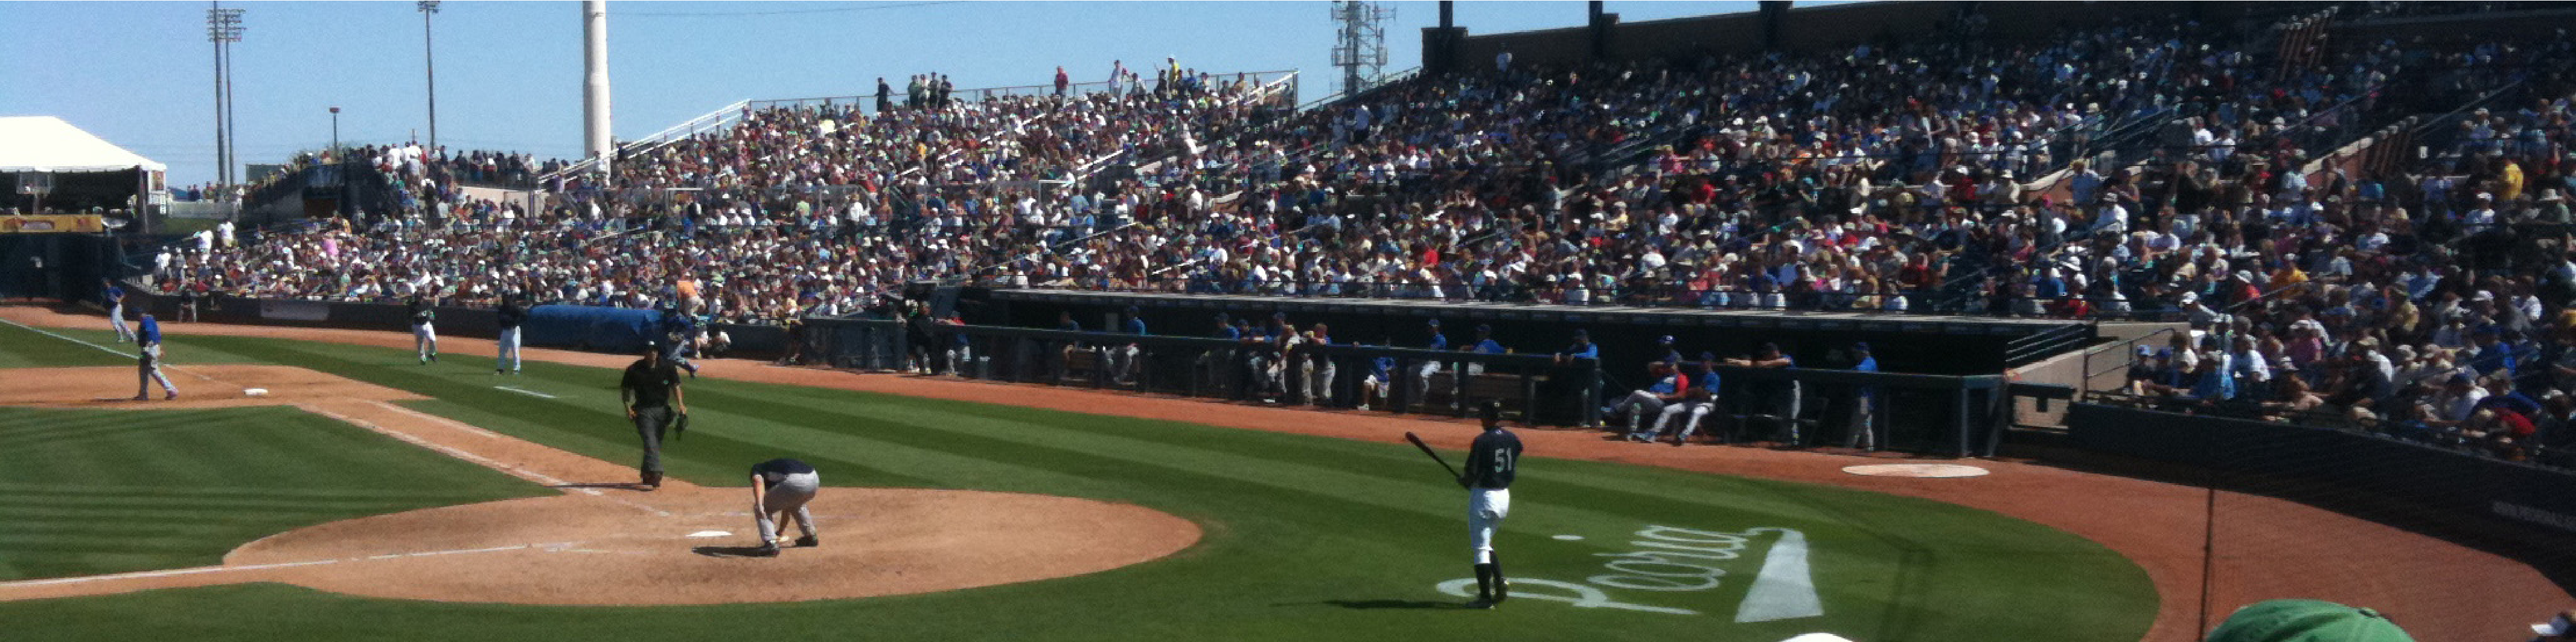
\includegraphics[width=\textwidth]{sampleteaser}
%   \caption{Seattle Mariners at Spring Training, 2010.}
%   \Description{Enjoying the baseball game from the third-base
%   seats. Ichiro Suzuki preparing to bat.}
%   \label{fig:teaser}
% \end{teaserfigure}

%%
%% This command processes the author and affiliation and title
%% information and builds the first part of the formatted document.
\maketitle


Deep neural networks (DNNs) have achieved strong performance on visual tasks.
The outstanding performance has been demonstrated by training a model with abundant and diverse labeled data
% ,~\eg,
~\cite{deng2009imagenet, lin2014microsoft}.
Despite the importance of data, machine learning researchers have focused mainly on the model and algorithms~\cite{sambasivan2021everyone}.
We should care about the data for training DNNs because unexpected influences can occur by data.
% and there is a lack of data debugging tools.
% We should first curate the dataset well for training the model because unexpected cascades can occur depending on the curated data~\cite{sambasivan2021everyone}.
% However, such abundant and well-curated labeled data are not available.
% The state-of-the-art DNNs suffer from much lower performance in certain types of classes or groups because of data imbalance.

We commonly encounter data imbalance problems categorized into \emph{class} or \emph{group} imbalance problems.
% The data imbalance problems we commonly encounter are mainly categorized into \emph{class} or \emph{group} imbalance problems.
Class imbalance means different data amounts in the classes.
Suppose that we collect animal images on the internet.
Images of rare animals may be found on search engines less than cats or dogs because of human bias for uploading their photograph~\footnote{For example, the number of search results of Tarsier is about 102 times less than Maltese in Google search engine.}.
Group imbalance, on the other hand, stands for different data amounts in the groups.
We may collect data depending on our environments, including preferences, country, and cultural backgrounds.
Suppose we collect a picture of human hands; then, the skin tones can be biased.
% The curator also may collect data depending on their environments\footnote{The skin tones of hands are imbalance~\cite{grady2022pressurevision}.}, such as preference, country, and cultural backgrounds, which implies the \emph{group imbalance problem}.
If we do not care about these biases, the collected dataset becomes imbalanced in terms of classes~\cite{cui2019class,zhang2023deep}, groups~\cite{whang2021responsible}, or both.
% These biases lead the collected dataset to be imbalanced in terms of classes~\cite{cui2019class,zhang2023deep} and groups~\cite{whang2021responsible}.
With such a dataset and the standard supervised learning algorithms based on empirical risk minimization (ERM) principle~\cite{vapnik1999nature}, the classifier will be trained to 
% will
be biased to majority classes~\cite{geirhos2020shortcut}.
Since these problems yield not only substantial performance degradation but also social or ethical issues with biases, researchers have independently developed various algorithms~\cite{arjovsky2019invariant,bahng2020learning,sagawa2019distributionally,teney2020unshuffling,tartaglione2021end, lee2021learning,LfF,liu2021just, kim2022learning,yao2022improving,hwang2022selecmix,kirichenko2023last,cao2019learning,ren2020balanced,samuel2021distributional, shen2016relay,park2022majority,kim2020m2m,liu2019large,zhang2022correct} to overcome these respective problems.

\begin{figure}[t]
    \centering
    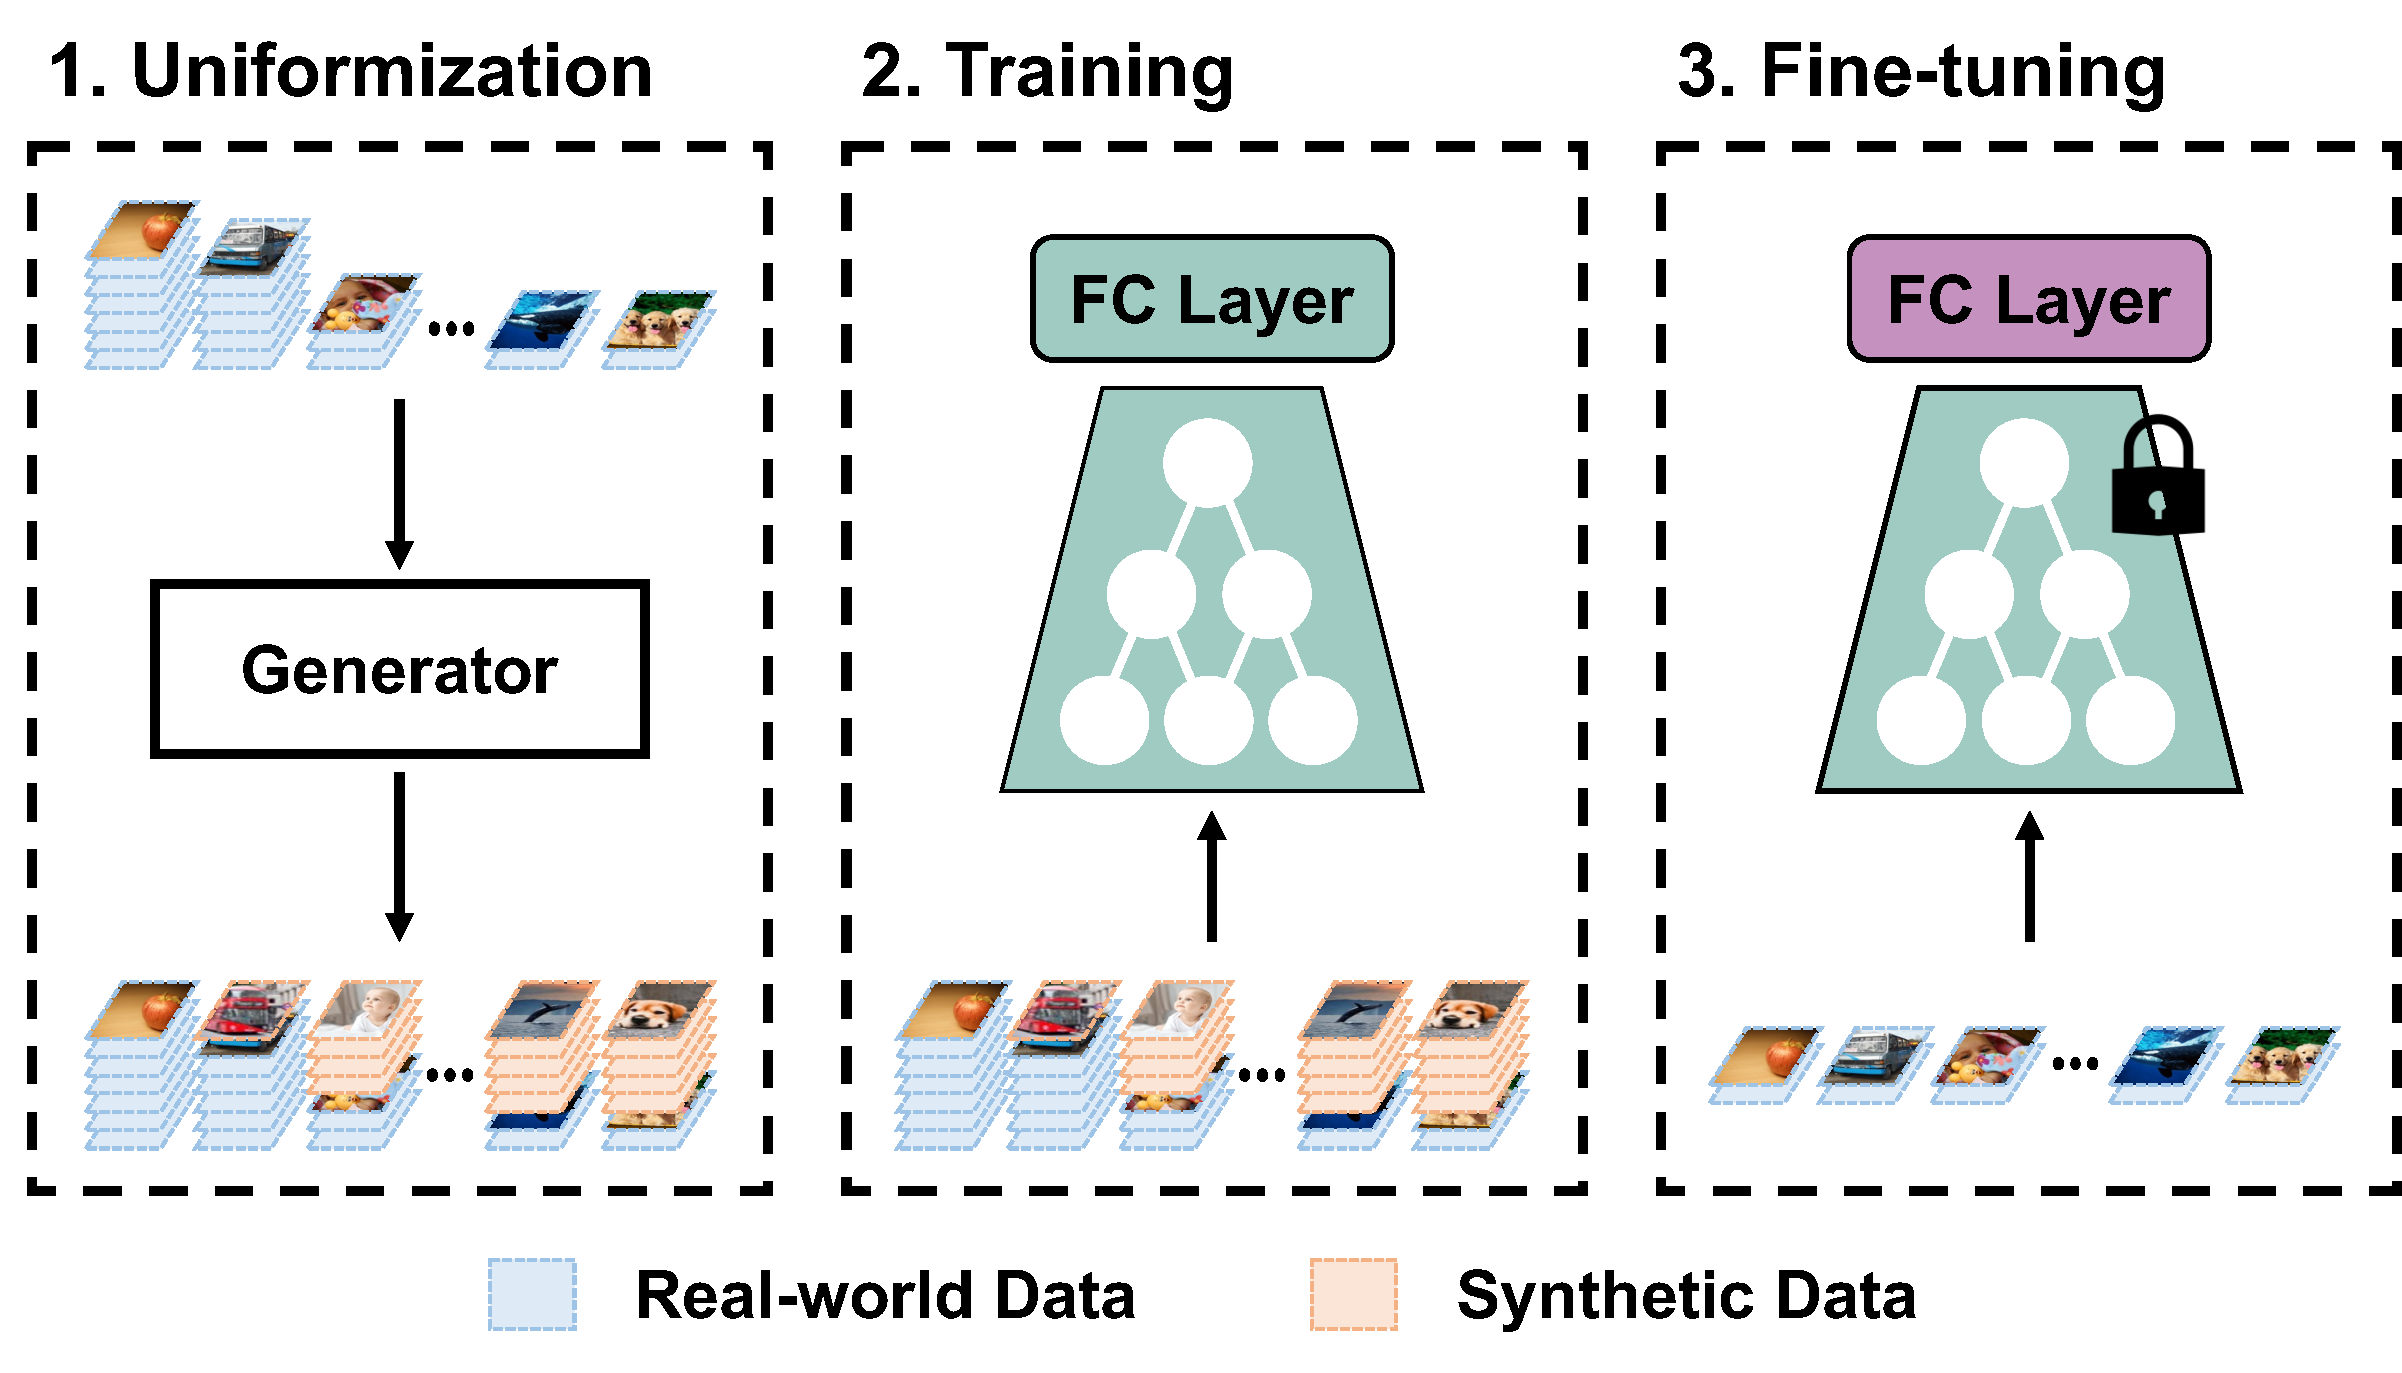
\includegraphics[width=1.0\linewidth]{figures/final.pdf}
    \caption{\textbf{Overview of SYNAuG process.}
    % \textcolor{realblue}{\textbf{legenBlue}} is the real-world data, and \textcolor{synorange}{\textbf{orange}} is the synthetic data.
    Given the imbalanced real-world data with the class labels, we first uniformize the imbalanced real data distribution by generating the synthetic samples that are conditioned on the class label.
    Second, we train a model with the uniformized training data.
    Finally, we fine-tune the last layer with the uniformly subsampled real-world data.}
    \label{fig:overview}
\end{figure}

In this work, we first uniformize the number of samples in each class using the recent text-to-image generative models before applying off-the-shelf task-specific algorithms.
% This takes a different direction, unlike the prior methods.
The prior studies 
% have reported improved performance over the state-of-the-art in their respective tasks.
% However, they use
work the limited, fixed, and bounded original dataset without adding more additional data and mainly focus on algorithmic approaches, such as reweighting~\cite{cao2019learning,ren2020balanced,samuel2021distributional,huang2019deep, ben2009robust, sagawa2019distributionally, jung2023reweighting}, resampling~\cite{shen2016relay,park2022majority,kim2020m2m,liu2019large, kamiran2012data, idrissi2022simple, roh2020fairbatch}, or augmentation~\cite{chuang2021fair, kim2020m2m, park2022majority}.
In contrast to the prior arts, we go beyond the fixed original dataset by exploiting
% , we exploit 
the generative diffusion models to synthesize data, which have recently shown potential as synthetic training data generation~\cite{poole2023dreamfusion, raj2023dreambooth3d, chen2023fantasia3d,trabucco2023effective, he2022synthetic, azizi2023synthetic}.
This allows us to tackle the fundamental bottleneck of data imbalance, \ie, data, rather than indirect ways of tackling learning algorithms or architectures.
It is a more natural way than restricting training data to the fixed dataset as in the prior arts.
% , which would be unnecessary in the generative model era.
% In the generative model era, we argue that restricting training data to the fixed dataset is impractical.
% Furthermore, data imbalance problems should be tackled from the data level before deploying algorithmic approaches.
% so that the practitioners take the controllability of data to mitigate and stabilize the base conditions of datasets.

As shown in \Fref{fig:overview}, we propose SYNAuG, exploiting the generative diffusion model to augment and make the original data distribution to be uniform distribution, \ie, uniformization.
% uniformize the original training data.
% , motivated by recent class imbalance approaches~\cite{kim2020m2m,he2022synthetic,kirichenko2023last}.
After training on the uniformized data composed of the original and synthetic data, we found that it is effective to use simple fine-tuning of the last layer with uniformly sub-sampled original data.
% after pretraining on the mixed dataset.
This outperforms the other strong baselines, including the baseline using the additional external web data as well as the competing methods on the long-tailed recognition benchmark, CIFAR100-LT, and the fairness benchmark, UTKFace.
In addition, we demonstrate the effectiveness of our method for improving the robustness of the classifier to spurious correlation.
We summarize our contributions as follows:
\begin{itemize}
    \item Proposing SYNAuG that uniformizes the given data distribution with synthetic data, beyond the given datasets;\vspace{-1mm}
    % not restricted to the given datasets;
    \item Demonstrating the effectiveness of SYNAuG on three distinctive data imbalance tasks: long-tailed recognition, model fairness, and robustness to spurious correlation;
    \vspace{-1mm}
    \item Reporting the observation of the importance of a few original samples when we use synthetic data together.
\end{itemize}




\section{Related Work}
To combat crimes in blockchain, transaction tracing is a critical task for blockchain security companies and the community. Current methods for blockchain transaction tracing are mainly designed for Bitcoin-like blockchain systems and heavily rely on expert experience. The most widely used transaction tracing method is Breath First Search (BFS) \cite{zhao2015graph,phetsouvanh2018egret}, and many related tools like skytrace\footnote{https://www.certik.com/skytrace} and coinholmes\footnote{https://trace.coinholmes.com} are available. Since BFS is insufficient to reveal the audit priority of different money tracking directions, the taint analysis technologies \cite{moser2014towards,tironsakkul2019probing,di2015bitconeview} have been proposed for bitcoin tracing according to the amount value and the order of multiple outputs in each transaction. However, these technologies rely on expert analysis and cannot automatically output the money flows from the source to the targets.

Based on the co-spending clustering heuristic in Bitcoin that the input addresses of the same transaction belong to the same entity \cite{Reid2013}, Huang et al. proposed to track the bitcoin flow of ransomware to when the money is being cashed out \cite{HuangTracking2018}.
% Tracking Ransomware End-to-end
Meiklejohn et al. \cite{meiklejohn2013fistful} utilized the change address heuristic to deanonymize the money flows in Bitcoin.
Moreover, some rule-based transaction tracing methods were proposed for cross-chain scenarios and mixing scenarios. For example, Yousaf et al. traced the cross-chain money flows by identifying the transactions which happen close in time and have similar amount value \cite{yousaf2019tracing}. 
However, these rule-based methods are designed for specific protocols and they are inapplicable to transaction tracing in account-based blockchains.

Personalized PageRank models the relevance of nodes in a network to a specific node, and has been widely used in web search \cite{page1999pagerank}, recommendations \cite{WTFGupta2013}, etc. Recently many variants and efficient approximations of personalized PageRank have been proposed for large-scale applications \cite{bojchevski2020scaling}. In this paper, we model the account-based blockchain data as a directed, weighted, temporal, and multi-relationship graph, and formalize the transaction tracing problem as a graph searching problem. We develop a scalable and intelligent transaction tracing tool for account-based blockchains based on personalized PageRank and its approximate solutions.
\section{Preliminaries} 
\label{sec:preliminaries}
% Before introducing our method, this section discusses the problem definition and provides preliminaries for this paper.

\subsection{Account-based blockchains}
% 不同于比特币系统采用基于UTXO的交易模型,以以太坊为首的基于账户的区块链系统xxxx
% 智能合约  DApp
% 由DApp引出Token  Token标准
% 去中心化交易所
Traditional Bitcoin-like blockchains are based on the transaction-centered model \cite{wu2021analysis} whose building block is unspent transaction output (UTXO), which is an indivisible cryptocurrency chunk locked to a specific owner. Each transaction has multiple inputs made up of UTXOs and multiple outputs, and there is a change address in the outputs used to receive the change.

Different from UTXO-based blockchains, account-based blockchain systems like Ethereum and BSC have the concept of account similar to that of traditional banking accounts. 
There are two kinds of accounts in account-based blockchains, namely external owned account (EOA) and smart contract account. 
Accounts are the initiators of blockchain transactions and record some dynamic state information including account balance. 
Especially, each smart contract account is associated with a piece of executable bytecode. There are also two types of transactions in the systems. 
A transaction triggered by an EOA is called external transaction, while a transaction triggered by an invocation of the function in a smart contract account is called internal transaction. 
In addition, an EOA can invoke functions of a smart contract in an external transaction and further result in many internal transactions. Transaction hash consisting of a set of numbers and letters is used to uniquely identify a particular transaction from or to an EOA.
Due to the support of smart contract, everyone can take the advantage of blockchain technology and build DApp projects in account-based blockchains.
Besides the native currency in blockchain systems, there are many third-party tokens representing assets, currency, or access rights of projects in the account-based blockchain ecosystem. 
To facilitate token development and exchange, some token standards are launched in blockchain trading systems, e.g., the ERC20 token standard in Ethereum. 
There are also many DeFi DApps that offer financial services such as token lending and exchange.
% 原来:
% 介绍加密数字货币包括原生币和Token
% There are two types of cryptocurrencies in account-based blockchains: native token and third-party token complimenting some standards.
% For Ethereum, the native token Ether and 
% 介绍什么是DeFi,DeFi世界中的交易语义有哪些

\subsection{Problem Definition}
\label{sec:problem_define}
The transaction tracing task in account-based blockchain trading systems aims to trace the money flows from a given source to the targets that gather the money awaiting cashing out and point the priority money flows for auditors to further verify manually. By modeling the blockchain transaction relationships as graph where nodes indicate the accounts and edges indicate the money flow relationships, we can formulate the transaction tracing problem as follows. 

% \begin{prbdef}
\textbf{Problem formulation.} \textit{Given a source node $s$ in a transaction graph $G$, the goal is to search a connected money transfer subgraph $G_{s}$ from $s$ to its money flow targets around the neighborhood of $s$. $G_{s}$ should contain as many target nodes as possible in the smallest possible size of graph for manual verification.}
% \end{prbdef}
% \textbf{Transaction network}.
% Transaction records on Blockchain trading systems like Bitcoin and Ethereum represent the relationship of cryptocurrency transfer among accounts.
% In this paper, transaction records from blockchain trading systems are represented as a transaction network $G = (V, E)$, where $V$ denotes the node set representing addresses, and $E$ denotes the edge set representing transaction relationships between addresses. 
% \textcolor{red}{Considering the amount, timestamp and token symbol of the transactions, each edge $e \in E$ can be defined as a five-tuple like $(u,v,w,t,b)$, where $u, v \in V$ denote the source and target nodes of $e$, respectively, $w$ denotes the transaction amount, $t$ denotes the transaction timestamp, and $b$ denotes the token symbol.}

% \textbf{Transaction Tracking on Blockchain}.

% The task of transaction tracking on blockchain can be modeled as graph searching on a transaction network, aiming at finding a subgraph of $s$ named \textbf{local tracking network}, denoted by $G_s$, which contains as many target nodes as possible.  
% As mentioned in the introduction, source nodes are usually deployers of various financial scams such as phishing, Ponzi scheme, blackmail, and extortion scams  \cite{wu2021analysis,oggier2020ego}, while the target nodes refer to the addresses which possess the laundered funds awaiting cashing out. 
% Due to the pseudonymous nature of blockchain, it is extremely difficult to trace the money flows between the source and target nodes and understand real-world entities behind the involved addresses and transactions.
% In some cases, some addresses are confirmed to be involved in illegal transaction activities by experts, and then the local tracking network should contain as many of these target nodes as possible.
% While sometimes, no prior information about target nodes is given, and then the local tracking network aims to contain the addresses with some particular labels (such as exchange deposit addresses) that are related to the source, providing us an opportunity to further infer the target nodes from these labeled nodes.


%identify all target nodes from the nodes related to the source node if the target nodes without given before.
% For example, the hackers steal the coin of the exchange, and we need to find the target nodes of hackers through transaction tracking methods.
% In addition, due to the pseudonymous nature of Blockchain trading systems, fetching the identity information for the transaction tracking model to know whether the target nodes have been found without given target nodes before is difficult.
%The goal of the transaction tracking problem can be given as follows:
%\begin{prbdef}

%The goal of this work is to find a network that contains as many nodes and transactions involved in the case as possible.

%Given a source node $s$ and a set of target nodes in a transaction network $G$, the goal of a transaction tracking model is to find a subgraph of $s$ named \textbf{local tracking network}, denoted by $G_s$, that contains as many target nodes as possible.
%\label{def:goal_tt_model}
%\end{prbdef}

% Transaction tracking tasks can be regarded as graph searching tasks on a transaction network, aiming at finding paths among the source node and the target nodes.
% In fact that it is difficult to know the target nodes before the transaction tracking task usually, for example, the hackers steal the coin of the exchange, and we need to find the target nodes of hackers through transaction tracking technology.
% In addition, due to the pseudonymity of transaction records on Blockchain, fetching the identity information of each node in the transaction network is impossible, which makes it difficult for the transaction tracking model to know whether the target node has been found without given target nodes before.

% \begin{prbdef}
% Base on this consideration, our goal is to construct a well-designed transaction tracking model able to find a subgraph named local tracking network from the source node, which satisfies:
% \begin{itemize}
%     \item The paths among the source node and the target nodes can be found, if the targets are given before.
%     \item The paths among the source node and the labeled nodes can be found, if the targets are unknown. 
%     And ensured that the target nodes can be found in the labeled node as much as possible.
% \end{itemize}
% \end{prbdef}

% Base on this consideration, the well-designed transaction tracking model will be able to find a subgraph that is most likely to contain the paths among the source node and the target nodes, even though the target node is not given in advance.
% Such a subgraph can be named a local tracking network.
% In this way, the effectiveness of the transaction tracking model can be evaluated by detecting whether there are enough label nodes in the local tracking network because experts can judge the action of the source node through the label nodes in the local tracking network, and then determine whether the label node is the target node through this action.

% Base on the Definition \ref{def:goal_tt_model}, we define the auditability of the local tracking network.
%According to whether the target nodes in the local tracking network can be identified, the auditability of a transaction network with a center of the source node is given as follow:
%\begin{prbdef}
%A transaction network with a center of the source node can be audited by a local tracking network, which satisfies: \textbf{1)} The paths among the source node and the target nodes can be found if the target nodes are given before. \textbf{2)} The paths among the source node and the labeled nodes can be found if the target nodes without given before, where the target nodes can be inferred from the labeled nodes.
% \end{itemize}
%\end{prbdef}
%For example, when it comes to a source node obtaining an amount of illegal money, laundering the money in a blockchain system and cashing them out via an exchange, the target node is the corresponding exchange deposit address without being given before. And we need to find out the paths between them.
%The transaction network can not be audited by the local tracking network in Figure \ref{fig:useless_tracking}, which misses the paths among the source and the target.
%On the contrary, the transaction network can be audited by the local tracking network as the Figure \ref{fig:useful_tracking}, which finds the path from the source to the target.

% It's reasonable that node $t$ is a target node of the source node $s$, because the stolen fund can be laundered on the exchange.
% There is a useless local tracking network as the Figure \ref{fig:useless_tracking} shows, which misses the path among $s$ and the labeled nodes, and we will not get more information from such a local tracking network about the target nodes of $s$.
% On the contrary, the local tracking network in Figure \ref{fig:useful_tracking} finds the path from $s$ to $t$, which is helpful for us to identify the target nodes.

% For example, when it comes to a source node $s$ obtaining the illegal fund and transfers the illegal fund to a node $t$ labeled as exchange.
% It's reasonable that node $t$ is a target node of the source node $s$, because the stolen fund can be laundered on the exchange.
% There is a useless local tracking network as the Figure \ref{fig:useless_tracking} shows, which misses the path among $s$ and the labeled nodes, and we will not get more information from such a local tracking network about the target nodes of $s$.
% On the contrary, the local tracking network in Figure \ref{fig:useful_tracking} finds the path from $s$ to $t$, which is helpful for us to identify the target nodes.

% In a word, the problem in this paper is how to design a transaction tracking model to complete the transaction tracking task in transaction networks on Blockchain.
% Here gives the definition of transaction tracking task as follow:\\
% \textbf{Definition}.
% \textit{Giving a transaction network $G$ and a source node $s$, the transaction tracking task is finding a local tracking network of $s$ that contains the paths among the source node and the target nodes.
% If the target nodes are unknown, ensured that the target nodes can be found in the labeled nodes of local tracking network as much as possible.}
% \begin{itemize}
%     \item If the target nodes are given, the transaction tracking task is finding a local tracking network of $s$ that contains the paths among the source node and the target nodes.
%     \item If the target nodes are unknown, the transaction tracking task is finding a local tracking network of $s$ that contains the paths among the source node and the labeled nodes ensured that the target nodes can be found in the labeled node as much as possible.
% \end{itemize}

\subsection{Approximate Personalized PageRank}
% To ensure the effectiveness of the tracking model, we usually need to define an importance measurement of other nodes in the network to the source node.
% or the probability of random walk to $u$ starting from $s$
\textbf{Personalized PageRank.} The personalized PageRank vector $\bm{p}_s$ of a source node $s$ in a graph $G=(V,E)$ is defined as the unique solution of Equation \ref{equ:ppr}, i.e.,
\begin{equation}
    \bm{p}_s = \alpha \bm{e}_s + (1-\alpha) \bm{p}_s M,
    \label{equ:ppr}
\end{equation}
where $\alpha$ is a teleport constant between 0 and 1, $\bm{e}_s$ is the indicator vector with a single nonzero element of 1 at $s$, $M$ is a transition matrix and $M=D^{-1}A$ where $D$ and $A$ are degree matrix and adjacency matrix. The definition of personalized PageRank is equivalent to simulating a random walk starting from $s$, and $\bm{p}_s$ is a probability vector where $\bm{p}_s(u)$ is the probability that a certain random walk beginning at $s$ terminates at $u$. 
% Let $\bm{p}_s$ denote the personalized PageRank vector of a source node $s$ in a graph $G=(V,E)$, where $\bm{p}_s(u)$ describes the relevance of a node $u$ to the source node $s$.

\textbf{Approximate personalized PageRank (APPR).} The first algorithm proposed to calculate personalized PageRank is power iteration \cite{page1999pagerank}, which requires high time complexity and not effective in large-scale networks.
Therefore, various efficient approximate solutions of personalized PageRank have been proposed, and the most widely used one is called the ``local push'' algorithm \cite{andersen2006local}. This algorithm starts with all probability residual on the source node of the graph, and pushes the residual to the neighbors iteratively. During the iterations, the residual of each node can be transformed into the relevance to the source node. Finally an estimate of $\bm{p}_s$ can be obtained. In the algorithm, a residual vector $\bm{r}_s$ is used to maintain the residual, where $\bm{r}_s(u)$ denotes the residual of node $u$. By setting $\bm{p}_s=\vec{0}$ and $\bm{r}_s=\bm{e}_s$ for initialization, the local push procedure updates the value of $\bm{p}_s(u)$ as follows:
\begin{equation}
    \begin{cases}
    & \bm{p}_s(u)=\bm{p}_s(u)+\alpha \bm{r}_s(u) \\
    & r(v)=r(v)+(1-\alpha)r(u) / d(u), \\
    % & \bm{r}_s(v)=\bm{r}_s(u)+\theta(u,v)\bm{r}_s(u)
    \end{cases},
    \label{equ:local_push_appr}
\end{equation}
where $v \in N(u)$ is the neighbor of $u$, and 
% the push factor $\theta(u,v)$ between $u$ and $v$ is defined as
% \begin{equation}
%     \theta(u,v)=\frac{1-\alpha}{d(u)},
% \end{equation}
% where 
$d(u)$ is the degree of $u$.
The local push procedure stops when the residual of each node in $G$ is within $\epsilon$.

\section{Proposed Approach}
\label{sec:proposed_approach}
% This section introduces the Push-Pop model and designs the TTR algorithm in Push-Pop model for blockchain transaction tracking.
This section introduces the architecture, implementation, and theoretical analysis of TRacer.

\subsection{Architecture Overview}
TRacer consists of three main modules including graph construction, graph expansion, and local community detection. Each module is described as follows:
\begin{itemize}
\item \textbf{Graph construction}: This module models the money transfer relationships between accounts as directed, weighted, temporal, and multi-relationship graphs.
% in which the nodes and the edges represent the accounts and the transactions in the blockchain, respectively.
\item \textbf{Graph expansion}: Since the blockchain data contains billions of transactions which is too large for common graph algorithms, this module aims to find a relevant subgraph from a risky source. The module contains four operations: \textit{\textbf{Expand}} collects all edges related to a given node, \textit{\textbf{Push}} merges the collected edges to the subgraph, \textit{\textbf{Rank}} computes the relevance of nodes in the subgraph to the source, and \textit{\textbf{Pop}} selects a node for expanding.
The graph expansion process terminates when the end condition is met.
\item \textbf{Local community detection}: This module \textit{\textbf{Extract}}s a local community of the source node from the expended subgraph, in which nodes have higher relevance to the source than nodes out of the community.
\end{itemize}

\subsection{Graph construction}
Since there are multiple types of tokens in account-based blockchain trading systems, we formulate the money transfer relationships among accounts into a directed, weighted, temporal, and multi-relationship graph $G=(V, E)$, where $V$ is the node set representing accounts, $E$ is the edge set representing the token transfer relationships.
% with $\varphi_E: E\rightarrow\{{\rm token \ types}\}$ for edge-type mapping
% , and $X$ denotes the set of attributes attached to edges including transaction hash (unique to the corresponding external transaction), amount, timestamp, and token symbol. 
An edge $e=(u,v,w,t,b,h)$ denotes that account $u$ transfer $w$ units token $b$ to account $v$ at timestamp $t$ with a transaction hash $h$. We define mapping functions $f_{src}$, $f_{tgt}$, $f_{amt}$, $f_{ts}$, and $f_{sym}$ to map each edge to its source, target, amount, timestamp, and token type respectively. There are multiple types of edges indicating the transfer relationships of different tokens.

In addition, many blockchain services such as decentralized exchanges act as the intermediary for token swap. 
To reveal the token flows after users interact with these services, we categorize the money transfer relationships into two patterns, namely \textbf{Xfer} and \textbf{Swap}.
As shown in Figure \ref{fig:Xfer}, accounts send or receive tokens through the Xfer pattern, and the related DeFi actions \cite{wu2021defiranger} in this pattern include: 1) \textbf{\textit{transfer}}: An account sends an amount of token to another account, 2) \textbf{\textit{minting}}: A token contract mints an amount of token to an account, and 3) \textbf{\textit{burning}}: An account burns an amount of token.
While accounts exchange tokens for other kinds of tokens through the Swap pattern as shown in Figure \ref{fig:Swap}, including three related DeFi actions: 1) \textbf{\textit{add liquidity}}: An account deposits an amount of token to a DeFi app, and receives a certain amount of Liquidity Provider (LP) token back, 2) \textbf{\textit{remove liquidity}}: An account sends an amount of LP token to a DeFi app for destroying and gets a certain amount of other tokens back, and 3) \textbf{\textit{trade}}: An account sells an amount of token A in a DeFi app for a certain amount of token B. We identify the transaction relationships involving both the sending of tokens and the receiving of another kind of tokens with the same hash as the relationships in the Swap pattern, and otherwise as the relationships in the Xfer pattern. 
% In this way, we define the pattern mapping for the edges in the transaction graph:
% \begin{equation}
%     P: E \rightarrow \{Xfer, Swap\}.
% \end{equation}

% In addition, considering the token transfer, there are two types of patterns for a transaction in TRacer, namely \textbf{Xfer} and \textbf{Swap}.
% A transaction is recognized as Swap if the transactions with the same transaction hash ensure an account sending and receiving tokens at the same time, otherwise Xfer.
% These two patterns are summarized from the transaction actions defined by token contracts and DeFi DApps. 
% Several main actions \cite{wu2021defiranger} are listed below:
% \begin{itemize}
%     \item \textbf{Transfer}: An account sends an amount of token to another account.
%     \item \textbf{Minting}: A token contract sends an amount of minted token to an account. 
%     \item \textbf{Burning}: An account sends an amount of token to a token contract for destroying.
%     \item \textbf{Add Liquidity}: An account deposits an amount of token to the DeFi app, which also sends its an amount of Liquidity Provider (LP) token to the account.
%     \item \textbf{Remove Liquidity}: An account sends an amount of LP token to a DeFi app for destroying, and the account gets a number of other tokens back.
%     \item \textbf{Trade}: An account sells an amount of token A in a DeFi app for a certain amount of token B.
% \end{itemize}

\begin{figure}[t]
    \centering
    \subfigure[The Xfer pattern]{
    
\includegraphics[width=0.3\linewidth]{figures/Xfer.png}
    \label{fig:Xfer}
    }
    \subfigure[The Swap pattern] {
    
\includegraphics[width=0.35\linewidth]{figures/Swap.png}
    \label{fig:Swap}
    }
    \caption{(a) Xfer: Sending or receiving tokens.
    % Transaction actions in this pattern include transfer, minting, and destroying. 
    (b) Swap: Exchanging tokens for other kinds of tokens. 
    % Transaction actions in this pattern include add liquidity, remove liquidity, and trade.
    }
\end{figure}

\subsection{Graph Expansion}
The graph expansion module aims to obtain a relevant subgraph expanded from a given seed via iterating four operations shown in Figure \ref{fig:TRacer}. In what follows, we introduce the design of these four operations.
\subsubsection{\textit{Push} and \textit{Rank}: Transaction Tracing Rank}
The \textit{Push} operation merges the expanded edges to the subgraph in each iteration. While \textit{Rank} calculates the relevance of nodes in the subgraph to the source.
% While Rank is the core operation of graph extension in TRace, which determines the rules for calculating the relevance of nodes to the source node in the subgraph.

We introduce APPR to calculate the node relevance. 
More specifically, the Rank operation executes the local push procedure for the incremental update of node relevance.
% Especially, according to some characteristics of the transaction graph in account-based blockchain, we design a novel local push procedure. 
% The relevance computed using this novel local push procedure is named \textbf{Transaction Tracing Rank} (TTR).
Based on the characteristics of blockchain transaction graph in account-based blockchains, we propose a novel local push algorithm named \textbf{\underline{T}ransaction \underline{T}racing \underline{R}ank (TTR)} to compute the node relevance in blockchain transaction graph. We develop four local push strategies in TTR, namely \textbf{tracing tendency, weighted pollution, temporal reasoning, and token redirection}. We use $r_s(u,t,b)$ to denote the residual of node $u$ brought from token $b \in B$ at timestamp $t \in \Gamma$, where $\Gamma$ is the timestamp set and $B$ is the token symbol set in the subgraph.
% In the local push procedure of TTR, the edge attributes of time and token symbol need to be considered, thus we use $r_s(u,t,b)$ to denote the residual attached with a timestamp $t \in \Gamma$ and a token symbol $b \in B$ in the node $u$, where $\Gamma$ is a set of timestamps, and $B$ is a set of token symbols.
% % the residual is stored by a dictionary structure with the definition below:
% % \begin{equation}
% %     r_s: V \times \Gamma \times B \rightarrow \mathbb{R},
% %     \label{req:residual_mapping}
% % \end{equation}
% % where $V$ denotes a set of nodes, $\Gamma$ denotes a set of timestamps, and $B$ denotes a set of token symbols.
In this way, the local push procedure in TTR is described as Algorithm \ref{alg:ttr_local_push}. During initialization, a part of the residual of node $u$ is transformed into the relevance (line 1). Moreover, other parts of the residual are pushed to the neighbors according to the four strategies.
% 伪代码备份
% \begin{algorithm}[t]
%     \caption{TTR local push}
%     \label{alg:ttr_local_push}
%     \begin{algorithmic}[1]
%         \REQUIRE Node $u$, edges $E(u)$ related to $u$, rank $\bm{p}_s$, residual $r_s$, timestamp set $\Gamma$, and token symbol set $B$.
%         \ENSURE The updated $\bm{p}_s$ and $r_s$.
%         %% 自环
%         \STATE $\bm{p}_s(u) = \bm{p}_s(u) + \alpha \sum\limits_{b \in B}\sum\limits_{t \in \Gamma}r_s(u,t,b)$
%         \STATE $r'_s(u,t,b)=r_s(u,t,b), r_s(u,t,b)=0$ for $\forall t\in \Gamma, \forall b\in B$.
%         \FOR{$(t,b)$ in $\Gamma \times B$}
%             \STATE $res = r'_s(u,t,b)$
%             %% 出边
%             \STATE $E_{out}(u)=$ the edges of $u$ output token $b$ after timestamp $t$.
%             \STATE $W_{out}=$ the sum of edge weight in $E_{out}(u)$.
%             \FOR{$e$ in $E_{out}(u)$}
%                 % \STATE $E'_{out}(u)=$ the out-edges of $u$ swapped from $e$ recursively.
%                 \STATE $E'_{out}(u)=\rho(\{e\}, E(u))$.
%                 \STATE $r_s(v_{e'},t_{e'},b_{e'})+=\frac{(1-\alpha) \beta w_e}{W_{out}|E'_{out}(u)|} \times res$ for $\forall e' \in E'_{out}(u)$
%             \ENDFOR
%             %% 入边
%             \STATE $E_{in}(u)=$ the edges of $u$ input token $b$ before timestamp $t$.
%             \STATE $W_{in}=$ the sum of edge weight in $E_{in}(u)$.
%             \FOR{$e$ in $E_{in}(u)$}
%                 % \STATE $E'_{in}(u)=$ the in-edges of $u$ swapped from $e$ recursively.
%                 \STATE $E'_{in}(u)=\rho(\{e\}, E(u))$.
%                 \STATE $r_s(v_{e'},t_{e'},b_{e'})+=\frac{(1-\alpha) (1-\beta) w_e}{W_{in}|E'_{in}(u)|} \times res$ for $\forall e' \in E'_{in}(u)$
%             \ENDFOR
%             \STATE $r_s(u,t,b)=(1-\alpha)\beta r'_s(u,t,b)$ if $|E_{out}(u)|==0$.
%             \STATE $r_s(u,t,b)=(1-\alpha)(1-\beta) r'_s(u,t,b)$ if $|E_{in}(u)|==0$.
%         \ENDFOR
%         \RETURN $\bm{p}_s, r_s$
%     \end{algorithmic}
% \end{algorithm}


\begin{algorithm}[t]
    \caption{TTR local push}
    \label{alg:ttr_local_push}
    \begin{algorithmic}[1]
        \REQUIRE Node $u$, edges $E(u)$ related to $u$, edge mapping functions $f_{src}$, $f_{tgt}$, $f_{amt}$, $f_{ts}$, $f_{sym}$, rank $\bm{p}_s$, residual $r_s$,
        timestamps $\Gamma$, token symbols $B$, 
        teleport constant $\alpha$, and tracing tendency $\beta$.
        \ENSURE The updated $\bm{p}_s$ and $r_s$.
        %% 自环
        % \STATE $\Gamma=\{f_{ts}(e) | e\in E(u)\}$
        % \STATE $B=\{f_{sym}(e) | e\in E(u)\}$
        \STATE $\bm{p}_s(u) = \bm{p}_s(u) + \alpha \sum\limits_{b \in B}\sum\limits_{t \in \Gamma}r_s(u,t,b)$
        \STATE $r'_s(u,t,b)=r_s(u,t,b), r_s(u,t,b)=0$, $\forall t\in \Gamma, \forall b\in B$.
        \FOR{$(t,b) \in \Gamma \times B$}
            % \STATE $res = r'_s(u,t,b)$
            %% 出边
            \STATE $E_{out}=\{e\in E(u)|f_{ts}(e)>t\wedge f_{src}(e)=u\wedge f_{sym}(e)=b\}$
            \STATE $E_{in}=\{e\in E(u)|f_{ts}(e)<t\wedge f_{tgt}(e)=u\wedge f_{sym}(e)=b\}$
            \FOR{$E' \in \{ E_{out}, E_{in} \}$}
                % \STATE $W=\sum\limits_{e \in E'}f_{amt}(e)$.
                \STATE $\gamma = \beta \ if \  E'==E_{out} \ else \ (1-\beta)$
                \FOR{$e \in E'$}
                    \STATE $E'_{\rho}=\rho(\{e\}, E(u))$ // obtained by Equation \ref{equation:token_redirect}
                    \FOR{$e' \in E'_{\rho}$}
                        \STATE $\Delta = \frac{(1-\alpha)\gamma f_{amt}(e)}{|E'_{\rho}|\sum\limits_{e ''\in E'}f_{amt}(e'')} r'_s(u,t,b)$
                        \STATE $v=f_{src}(e') \ if \ E'==E_{in} \ else \ f_{tgt}(e')$
                        \STATE $r_s(v,f_{ts}(e'),f_{sym}(e'))+=\Delta$
                    \ENDFOR
                    % \STATE $r_s(f_{amt}(e'),f_{ts}(e'),f_{sym}(e'))+=\frac{(1-\alpha)\gamma f_{amt}(e)}{|E'_{\rho}|\sum\limits_{e \in E'}f_{amt}(e)} r'_s(u,t,b)$ for $e'\in E'_{\rho}$
                \ENDFOR
                \STATE $r_s(u,t,b)=(1-\alpha)\gamma r'_s(u,t,b)$ if $|E'|==0$.
            \ENDFOR
            % \STATE $r_s(u,t,b)=(1-\alpha)\beta r'_s(u,t,b)$ if $|E_{out}(u)|==0$.
            % \STATE $r_s(u,t,b)=(1-\alpha)(1-\beta) r'_s(u,t,b)$ if $|E_{in}(u)|==0$.
        \ENDFOR
        \RETURN $\bm{p}_s, r_s$
    \end{algorithmic}
\end{algorithm}
% In this way, the TTR local push procedure in a node $u$ can be described by the equations below:
% \begin{equation}
%     \begin{cases}
%         & \Delta \bm{p}_s(u) = \alpha \sum\limits_{b \in B} \sum\limits_{t \in \Gamma} r_s(u,t,b) \\ 
%         & \Delta r_s(v_{out},t,b) = (1-\alpha)\beta \rho 
%         \begin{pmatrix}
%         b, \theta 
%             \begin{pmatrix}
%             v_{out}, r_s, \tau(t,E(u))
%             \end{pmatrix}
%         \end{pmatrix}
%          \\ 
%         & \Delta r_s(v_{in},t,b) = (1-\alpha)(1-\beta) \rho
%         \begin{pmatrix}
%         b, \theta 
%             \begin{pmatrix}
%             v_{in}, r_s, \tau(t,E(u))
%             \end{pmatrix}
%         \end{pmatrix}
%     \end{cases},
% \end{equation}
% in which $t\in \Gamma$, $b \in B$, $v_{out} \in N_{out}(u)$ and $v_{in} \in N_{in}(u)$ denote out-degree neighbor and in-degree neighbor of $u$ respectively, $\beta$ denotes the tracing tendency coefficient controlling the attention for different neighbors, $\theta$ denotes a weight pollution function focusing on distributing the residual by edge weight, $\tau$ denotes the temporal reasoning function aiming to select edges with specific timestamps, $\rho$ denotes the token redirection function for processing the transaction patterns, and $E(u)$ denotes the edges related to the node $u$.

\textbf{Tracing tendency}.
Since a money transfer relationship between accounts is directed, the attention to in-degree neighbors and out-degree neighbors during the local push procedure can be different.
% For example, tracing for the target of the fund flows oriented from a particular source needs to pay more attention to its out-degree neighbors, while tracing for the source of money needs to pay more attention to the in-degree neighbors.
In most cases, tracing for the destinations of money flows oriented from a particular source needs to pay more attention to the out-degree neighbors. Therefore, we define an attention coefficient $0 \leq \beta \leq 1$. During the residual propagation, the out-degree neighbors in a transaction relationship can get a higher residual when $\beta > 0.5$, and the in-degree neighbors can receive a higher residual when $\beta < 0.5$. As Figure \ref{fig:TTR_strategies}(a) shows, the in-degree neighbors and the out-degree neighbors obtain a different weight in this strategy. Line 6-17 in Algorithm \ref{alg:ttr_local_push} describe the residual propagation procedure of different directions with the attention coefficient assigned at line 7. 
%Therefore, considering the transaction graph $G$ is directed and giving a tracing tendency coefficient $0 \leq \beta \leq 1$, the out-degree neighbors in a transaction relationship get a higher residual when $\beta > 0.5$ for tracing the target of the fund flow, and the in-degree neighbors in a transaction relationship get a higher residual when $\beta < 0.5$ for tracing the source of the fund flow.
% As Figure \ref{fig:tracing_tendency} shows, the out-degree neighbors of a node $u$ get a higher residual than the in-degree neighbors, when $\beta > 0.5$.
% In this way, the residual is split for pushing to out-degree neighbors and in-degree neighbors with different coefficients being $\beta$ and $1-\beta$ (line 7) in Algorithm \ref{alg:ttr_local_push}.

\textbf{Weighted pollution}. 
% Traditional APPR pushes the residual of a node to the neighbors by considering an equal weight during a local push procedure. 
% However, in a transaction relationship, the transaction strength is usually weighted by the transaction amount. 
% Note that the edge strength is usually weighted by the transaction amount.
In blockchain transaction graph, the strength of money transfer relationships is weighted by the transaction amount. For each node, a neighbor trading a larger amount of money with this node is considered to be more relevant to the node. 
% Therefore, by considering the transaction graph $G$ is weighted with the transaction amount information as the weight, 
Therefore, in this strategy we take the weight of the money transfer relationships into account. Figure \ref{fig:TTR_strategies}(b) shows an example of this strategy that neighbors of $u$ associated by edges with greater weight can obtain more residual during the propagation.
In this way, the residual of a node is distributed to each neighbor associated by edge $e \in E'$ according to the ratio of edge weight $f_{amt}(e) / \sum_{e'' \in E'}f_{amt}(e'')$ as shown in Algorithm \ref{alg:ttr_local_push} line 11, where $E'$ is the set of edges.

\textbf{Temporal reasoning}.
Blockchain transactions are recorded in blocks chronologically. Each block contains a specific timestamp. 
% Since the fund flow transferring process is dynamic, the transaction time information can be taken into consideration in the local push procedure.
With the timestamp information, tracing for the targets of money flows usually follows the paths with increasing timestamps, while tracing back to the source of money flows follows the paths with decreasing timestamps.
Therefore, in this strategy we take the temporal information into consideration. For example in Figure \ref{fig:TTR_strategies}(c), the residual from the input transaction at $t2$ is pushed out through the outgoing edges after $t2$ and the incoming edge before $t2$. Algorithm \ref{alg:ttr_local_push} line 4-5 show the edge set for residual propagation that satisfies this strategy.
% The timestamp is used to restrict the edges for pushing (line 4, 5) in Algorithm \ref{alg:ttr_local_push}.
Moreover, the residual is pushed to the node itself if the edge set is empty in Algorithm \ref{alg:ttr_local_push} line 16, indicating that the funds have not been transferred from the node.

\begin{figure}[t]
    \centering
    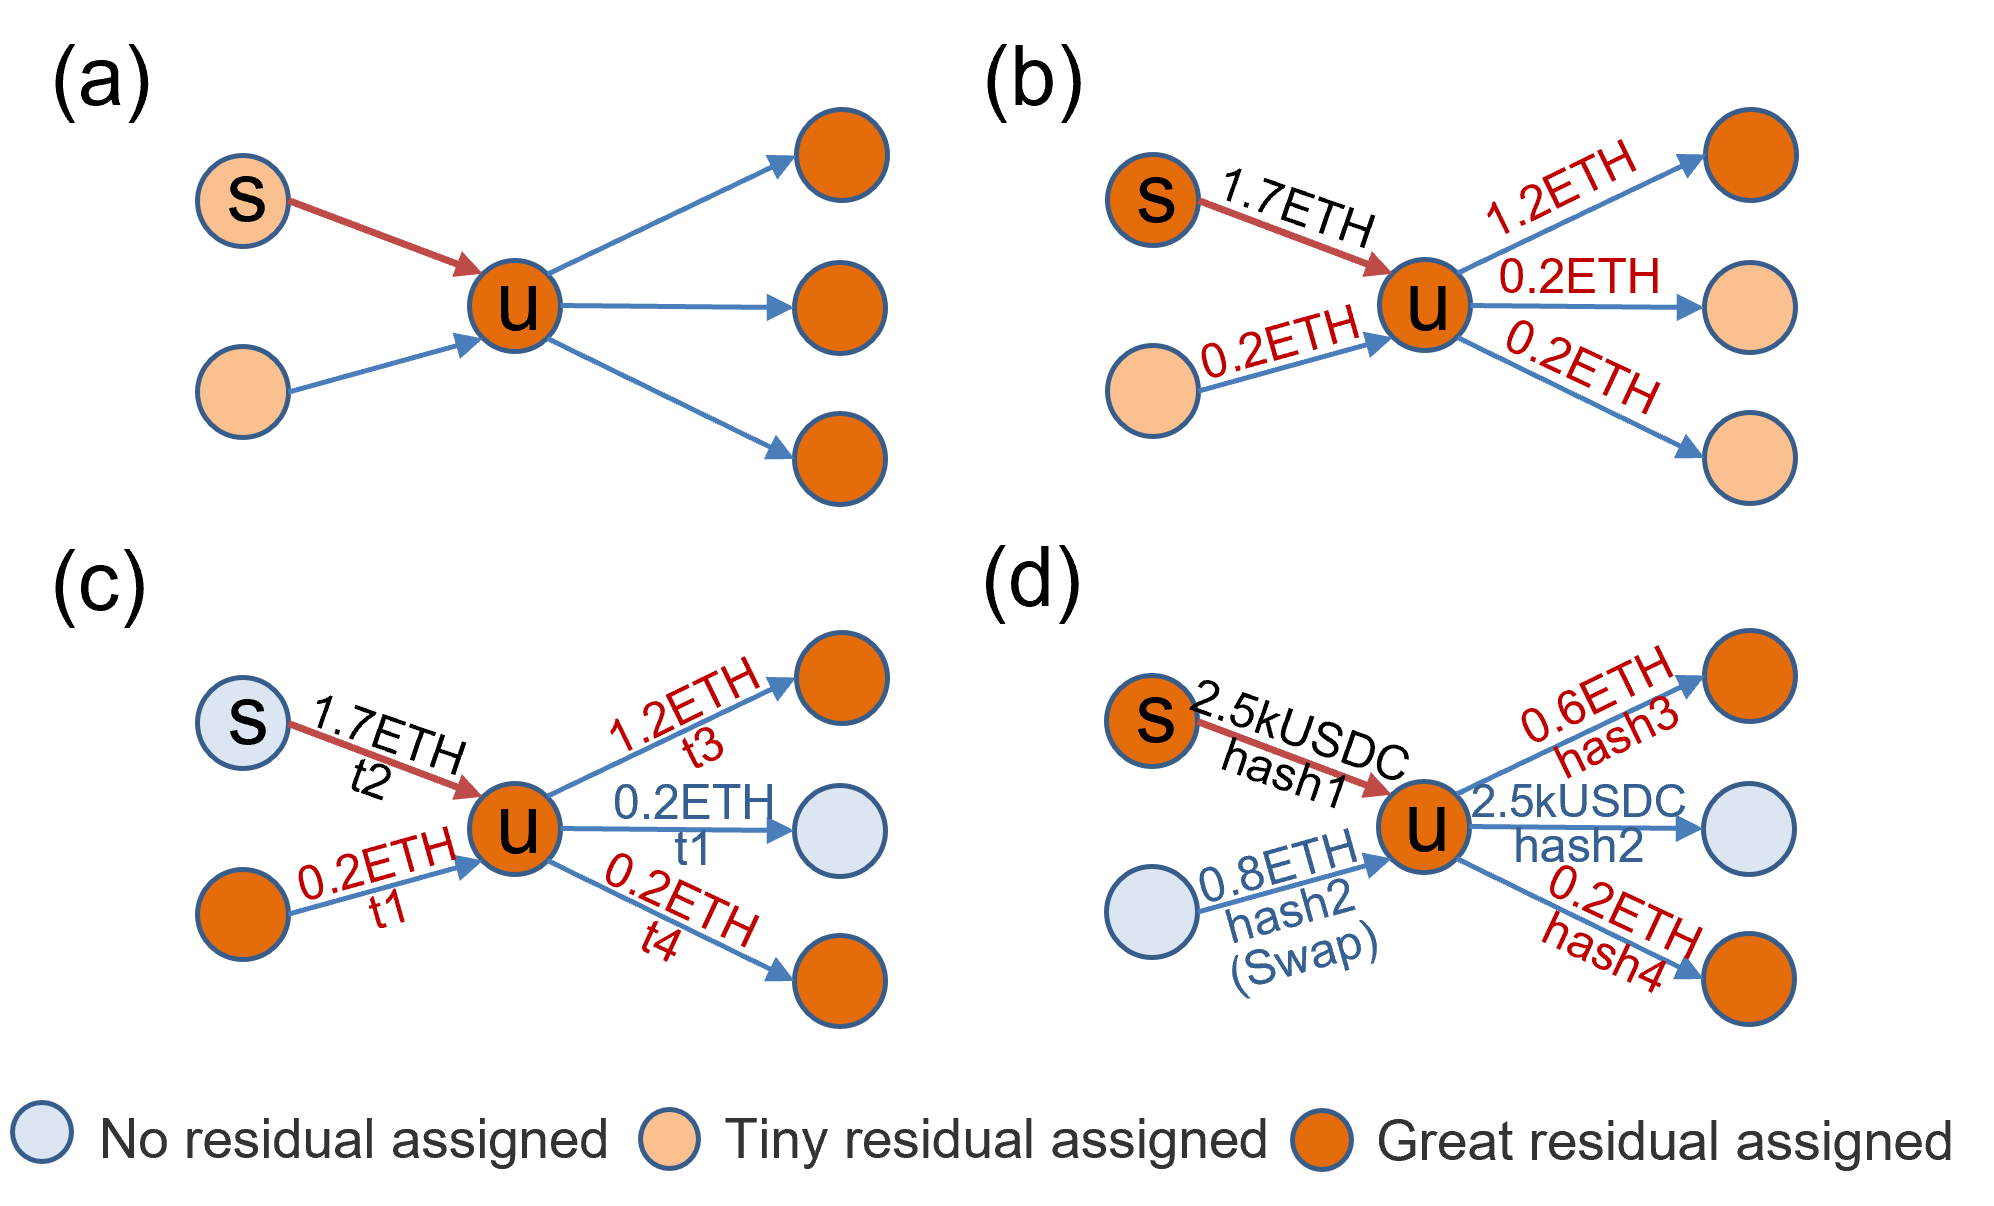
\includegraphics[width=0.9\linewidth]{figures/TTRstrategies.png}
    \caption{(a) Tracing tendency. 
    Different attention is assigned to the out-degree neighbors and in-degree neighbors.
    (b) Weighted pollution. The higher the edge weight, the closer the relationship. 
    (c) Temporal reasoning. Tracing money flow in chronological order, and $t1<t2<t3<t4$ in this example. 
    (d) Token redirection. Uncovering the token flows even though there exist complex DeFi actions in the Swap pattern.}
    \label{fig:TTR_strategies}
\end{figure}

% \begin{figure}[t]
%     \centering
%     \subfigure[Tracing tendency]{
%     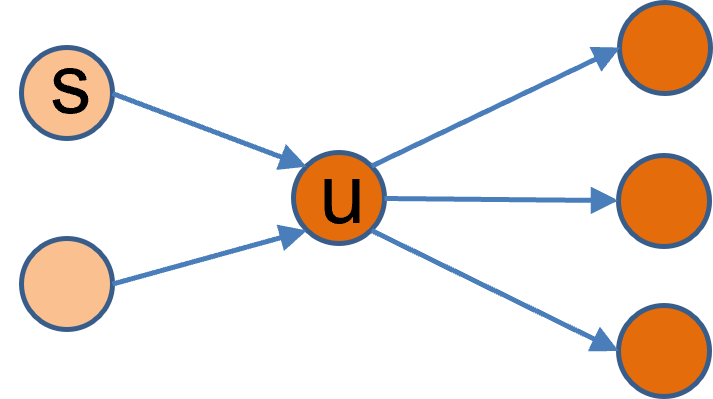
\includegraphics[width=0.35\linewidth]{figures/tracing_tendency.png}
%     \label{fig:tracing_tendency}
%     }
%     \subfigure[Weight pollution]{
%     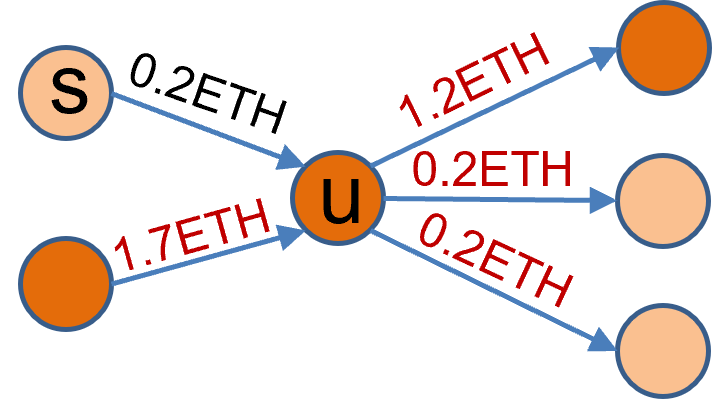
\includegraphics[width=0.35\linewidth]{figures/weight_pollution.png}
%     \label{fig:weight_pollution}
%     }
%     \subfigure[Temporal reasoning]{
%     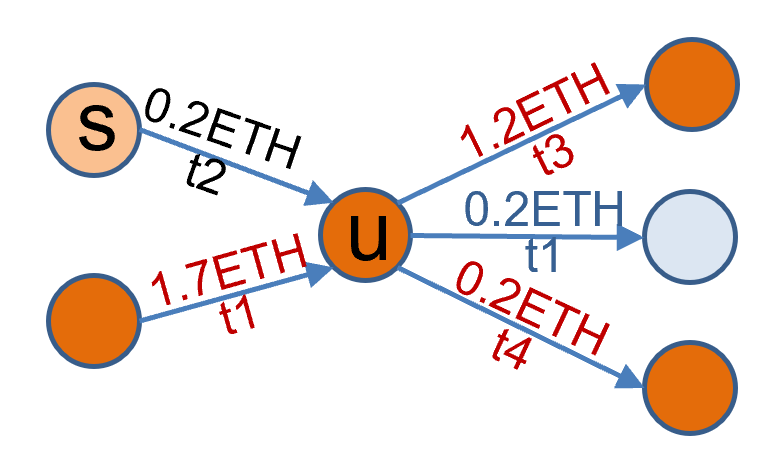
\includegraphics[width=0.35\linewidth]{figures/temporal_reasoning.png}
%     \label{fig:temporal_reasoning}
%     }
%     \subfigure[Token redirection]{
%     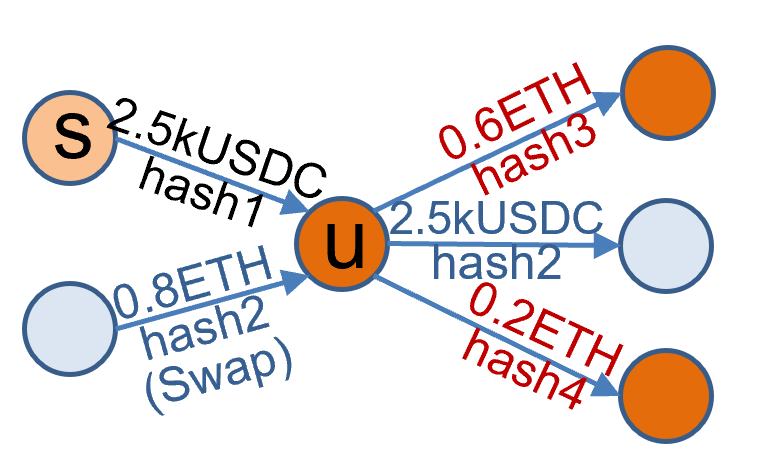
\includegraphics[width=0.35\linewidth]{figures/token_redirection.png}
%     \label{fig:token_redirection}
%     }
%     \caption{
%     (a) Tracing tendency. Different attention is assigned to the out-degree neighbors and in-degree neighbors.
%     (b) Weight pollution. The higher the edge weight, the closer the relationship. 
%     (c) Temporal reasoning. Tracing money flow in chronological order, and $t1<t2<t3<t4$ in this example. 
%     (d) Token redirection. Uncovering the token flow even though there exist complex transaction actions in the Swap pattern.
%     }
% \end{figure}

\textbf{Token redirection}.
% Besides native currency transfers, the transactions of account-based blockchain contain a large number of token transfers, while token redirection makes effort to reveal the real flow of interesting tokens.
This strategy makes the effort to uncover the flow of interesting tokens based on the transaction patterns of Xfer and Swap.
% In TRacer, the transaction patterns of Xfer and Swap are taken into consideration when it comes to tracing the token fund flow.
As Figure \ref{fig:TTR_strategies}(d) shows, the residual of node $u$ brought from the USDC token in an Xfer edge with hash1 should be pushed through the edges with hash3 and hash4, rather than the USDC outgoing edge with hash2. Since the edges with hash2 are in a Swap pattern and swapped the USDC token into ETH.
% As Figure \ref{fig:token_redirection} shows, the residual with USDC token received by the node $u$ in an Xfer edge with hash1 should have been pushed to the out-degree neighbor by the edge with USDC and hash2, but considering the edge with USDC and hash2 for redirection, the residual is pushed through the output edges with hash3 and hash4.
To achieve the redirection of token flows in complex transaction actions, we define a recursive function $\rho(\cdot,\cdot)$ which can find the initial state of a set of incoming edges before the Swap operations and the final state of a set of outgoing edges after the Swap operations within a node. For example, the initial state before Swap of the incoming edge with hash2 in Figure \ref{fig:TTR_strategies}(d) is the incoming edge with hash1, and the final state after Swap of the outgoing edge with hash2 is the outgoing edges with hash3 and hash4. More specifically, as shown in Algorithm \ref{alg:ttr_local_push} line 8-14, the residual of a specific token should be pushed through the redirected edges. Therefore, $\rho(\cdot,\cdot)$ satisfies the following recursive equation:
\begin{equation}\label{equation:token_redirect}
    \rho(\mathcal{E}, E(u))=\mathcal{E}_{xfer} \cup \rho(\bigcup\limits_{e \in \mathcal{E}_{swap}} redirect(e), E(u)),    
\end{equation}
where $\mathcal{E}$ is a set of edges for redirection, $\mathcal{E}_{xfer} \subset \mathcal{E}$ is a set of Xfer edges, $\mathcal{E}_{swap} \subset \mathcal{E}$ is a set of Swap edges, and $redirect(\cdot)$ selects the edges in the token types before/after Swap for incoming/outgoing edges $e \in \mathcal{E}_{swap}$ from edges $E(u)$ related to $u$.
% , which satisfies $f_{src}(e')=f_{src}(e)=u$ or $f_{tgt}(e')=f_{tgt}(e)=u$ for $\forall e' \in redirect(e)$.
% redirect selects the output/input edges from $E(u)$ with the swapped token symbol of the output/input edge $e \in \mathcal{E}_{swap}$.
Especially, $\rho(\emptyset, E(u)) = \emptyset$.

\subsubsection{\textit{Pop} and \textit{Expand}: Greedy Selection}
The \textit{Pop} operation selects a node from the subgraph for the next round expansion iteration, and the \textit{Expand} operation expands from a node by collecting all the related edges of this node.
% The \textit{Pop} operation selects a node with high priority from the subgraph in graph expansion, while \textit{Expand} collects all edges related to the selected node.
% In TRacer, the priority of the nodes is residual, where the node with a higher residual has a greater priority.
Note that the graph expansion in TRacer terminates when the residual of all nodes in the subgraph is below a threshold $\epsilon \in (0,1)$, i.e.,
\begin{equation}
    \max\limits_{u \in V}(\sum\limits_{t \in \Gamma}\sum\limits_{b \in B}r_s(u,t,b)) < \epsilon.
    \label{equ:end_cond}
\end{equation}
Thus we proposed the \textbf{greedy selection} for the \textit{Pop} operation to achieve the condition in Equation \ref{equ:end_cond}, i.e., the \textit{Pop} operation selects the node in the subgraph with the highest residual.
% Thus we proposed two types of node selection rules for the \textit{Pop} operation to achieve the condition in Equation \ref{equ:end_cond}, namely greedy selection, and group selection:
% \begin{itemize}
%     \item \textbf{Greedy selection}: Select one node in the subgraph with the highest residual.
%     \item \textbf{Group selection}: Select all nodes in the subgraph where the residual of every node is greater than $\epsilon$.
% \end{itemize}
% In our implementation, the greedy selection is chosen for \textit{Pop} operation enabled to reduce the pressure of data access in \textit{Expand}.

% \subsection{\textit{Extract}: Local Community Detection}
\subsection{Local Community Detection}
Referring to Figure~\ref{fig:TRacer}, the \textit{Extract} operation employs local community detection to construct a small-scale local community from the expanded graph. For a particular risky source node, the importance rank of the nodes within the local community is significantly higher than the external nodes, making it easy for further expert auditing.


The less conductance \cite{andersen2006local, andersen2007local} of the local community, the higher rank of the nodes in the local community than external nodes, in which the conductance is:
\begin{equation}
    \Phi(S)=\frac{\bm{p}_s(\partial(S))}{\bm{p}_s(S)},
\end{equation}
where $S$ denotes the nodes of the local community, the boundary $\partial(S)=\{ v| (u,v) \in E \land u \in S \land v \in \bar{S} \}$, $\bar{S}$ is the complement of $S$ and $\bm{p}_s(S)=\sum_{u \in S}\bm{p}_s(u)$ denotes the sum of rank over each node in the local community.
Given a specific threshold $\varphi > 0$ for conductance, the local community detection finds the local community satisfying:
\begin{equation}
    \Phi(S) < \varphi.
    \label{equ:local_comm_cond}
\end{equation}
With $S=\{s\}$ as the initialization, Algorithm \ref{alg:ttr_local_comm} describes how to find the local community satisfied the Equation \ref{equ:local_comm_cond}.
\begin{algorithm}[t]
    \caption{TTR-based Local Community Detection}
    \label{alg:ttr_local_comm}
    \begin{algorithmic}[1]
        \REQUIRE The source node $s$, the subgraph of graph expansion $G_s=(V_s, E_s)$, and the TTR score vector $\bm{p}_s$.
        \ENSURE The local community with nodes set $S$.
        \STATE $S = \{ s \}$
        \STATE $\bar{S} = V_s \setminus S$
        \WHILE{$\Phi(S) \geq \varphi$}
            \STATE $u =\mathop{\arg\max}_{v\in\bar{S}}\bm{p}_s(v)$
            % \STATE $u =$ the node with the highest rank in $\bar{S}$
            \STATE $S = S \cup \{ u \}$
            \STATE $\bar{S} = \bar{S} \setminus \{ u \}$
        \ENDWHILE
        \RETURN $G_s.subgraph(S)$
    \end{algorithmic}
\end{algorithm}
\subsection{Theoretical properties}
In this part, we discuss the theoretical properties of TRacer, and prove that our method is able to finish the transaction tracing task in large-scale transaction graphs with a constant time cost. Besides, we discuss the upper limit of the tracing depth in TRacer.

As the description in Proposition \ref{pot:cost}, the cost of TRacer is independent of the graph size, indicating that TRacer is able to trace on the large-scale transaction graph with a low cost.
\begin{proposition}
\label{pot:cost}
The iteration of graph expansion runs $O(\frac{1}{\epsilon \alpha})$ times, and the number of nodes with non-zero values in the output TTR score is at most $O(\frac{1}{\epsilon \alpha})$, which guarantees the cost of local community detection is $O(\frac{1}{\epsilon \alpha})$.
\end{proposition}
\begin{proof}
This follows from Andersen et al. \cite{andersen2006local}, Lemma 2.
\end{proof}

In addition, what depth can TRacer trace in a transaction graph from the source node is described in Proposition \ref{pot:max_depth}.
% where the higher order of the neighbor, the longer distance between the source node and this neighbor.
\begin{proposition}
\label{pot:max_depth}
An $n$-hop neighbor of the source node can be found in the graph obtained by graph expansion, in which $n$ satisfies:
\begin{equation}
    n \leq \frac{log(\epsilon)}{log(1-\alpha)} + 1.
\end{equation}
\end{proposition}
\begin{proof}
In order to maximize the rank of the neighbors far away from the source node, $\alpha$ needs to be as small as possible, and $\beta$ needs to be as close as possible to 0 or 1, which ensures that the residual can be pushed to a specific direction.
Let the sum of residual pushed from the source node $s$ to the $n$-hop neighbors be $r^{(n)}$.
Considering $\beta=1$ here, $r^{(n)}$ can be obtained by:
\begin{equation}
    \begin{cases}
        & r^{(1)}=(1-\alpha), \\
        & r^{(2)} \geq (1-\alpha)(r^{(1)}-k_1 \epsilon)=(1-\alpha)^2-(1-\alpha)k_1 \epsilon, \\
        & ...... \\
        & r^{(n)} \geq (1-\alpha)(r^{(n-1)}-k_{n-1} \epsilon) \\
        & \ \ \ \ \ \ \ \ =(1-\alpha)^n-\sum\limits_{i=1}^{n-1}(1-\alpha)^{n-i}k_{n-i} \epsilon, \\
    \end{cases}
\end{equation}
where $k_i$ represents the number of nodes with residual less than $\epsilon$ in the $i$-order neighbors of the source node.
Therefore, $r^{(n)}$ obtains the maximum value when:
\begin{equation}
    \sum\limits_{i=1}^{n-1}(1-\alpha)^{n-i}k_{n-i} \epsilon = 0,
\end{equation}
which means the residual of each $i$-order node is greater or equal than $\epsilon$. 
This situation exists when the source node is in a path-like graph, whose adjacency matrix $A$ satisfies $A(i,i+1)=1$ and other elements are $0$.
Considering the end condition of the local push procedure, the residual of $n$-hop neighbors is:
\begin{equation}
\begin{cases}
    & (1-\alpha)^n < \epsilon\\
    & (1-\alpha)^{n-1} \geq \epsilon \\
\end{cases}
    % r^{(n)}=(1-\alpha)^n \geq \epsilon
    \Rightarrow 
    \frac{log(\epsilon)}{log(1-\alpha)} < n \leq \frac{log(\epsilon)}{log(1-\alpha)} + 1.
    % n \leq \frac{log(\epsilon)}{log(1-\alpha)}.
\end{equation}
\end{proof}
% ------------ 旧版内容 ------------
% \subsection{Push-Pop Model}
% In this paper, we propose a general framework called Push-Pop model for transaction tracking on blockchain trading systems. 
% As shown in Figure \ref{fig:push_pop_model}, the Push-Pop model starts from the source node $s$ with a specific transaction tracking strategy $T$, builds a witnessed network iteratively, and finds a subgraph from the witnessed network as the local tracking network of the source node finally.
% Here we aim to find a local tracking network containing as many target nodes as possible.
% The witnessed network of a source node under a transaction tracking strategy $T$ is defined as $G_s^T=(V_s^T,E_s^T,PR_s^T)$, where $V_s^T$ and $E_s^T$ denote the nodes and edges of $G_s^T$ respectively while $PR_s^T$ is a vector denoting the priority of all nodes in $G_s^T$.

% To build $G_s^T$ for source node $s$, the steps of Push-Pop model are defined as follows:
% \begin{enumerate}
%     \item \textit{initialize}: Let $V_s^{T}=\{ s \}$, $E_s^{T}=\emptyset$, and $PR_s^T(s)=1$.
%     \item \textit{pop}: Output the node $v$ with the highest priority from the node set $V_s^{T}$.
%     \item \textit{expand}: Query the edges $E(v)$ related to $v$ and the neighbor nodes $N(v)$ of $v$.
%     \item \textit{push}: Update the witnessed network $G_s^T$ in which $E_s^{T}=E_s^{T} \cup E(v)$, $V_s^{T}=V_s^{T} \cup N(v)$, and employ the transaction tracking strategy $T$ to rank the priority of nodes in $V_s^T$ for updating $PR_s^{T}$. If the end condition of $T$ is not satisfies, go to step 2.
%     \item \textit{extract}: Output a subgraph of the witnessed network $G_s^T$ as the local tracking network $G_s$.
% \end{enumerate}

% % Therefore, the Push-Pop model is defined as Algorithm \ref{alg:push_pop}.
% Obviously, the effectiveness of Push-Pop model depends on the transaction tracking strategy, and how to design an effective strategy will be discussed in the next part.
% % \begin{algorithm}[htb]
% %     \caption{Push-Pop Model}
% %     \label{alg:push_pop}
% %     \begin{algorithmic}[1]
% %         \REQUIRE The transaction network $G$, the source node $s$, transaction tracking strategy $T$
% %         \ENSURE The local tracking network captured by $T$
% %         \STATE $T.V.init(s)$
% %         \WHILE{$T.V.hasNext()$}
% %             \STATE $u = T.V.pop()$
% %             \STATE $E(u) = T.expand(u)$
% %             \STATE $T.V.push(E(u))$
% %         \ENDWHILE
% %         \RETURN $T.extract(G_T)$
% %     \end{algorithmic}
% % \end{algorithm}

% \subsection{Transaction Tracking Rank Algorithm}
% The TTR algorithm improves the local push procedure of APPR to enable that nodes related to the source node in a given transaction network $G=(V,E)$ can have a higher estimate of $\bm{p}_s$.
% According to the attributes of transaction network, we design three local push strategies in the TTR algorithm.

% % \begin{figure*}[htb]
% %     \centering
% %     \subfigure[tracking tendency]{
% %         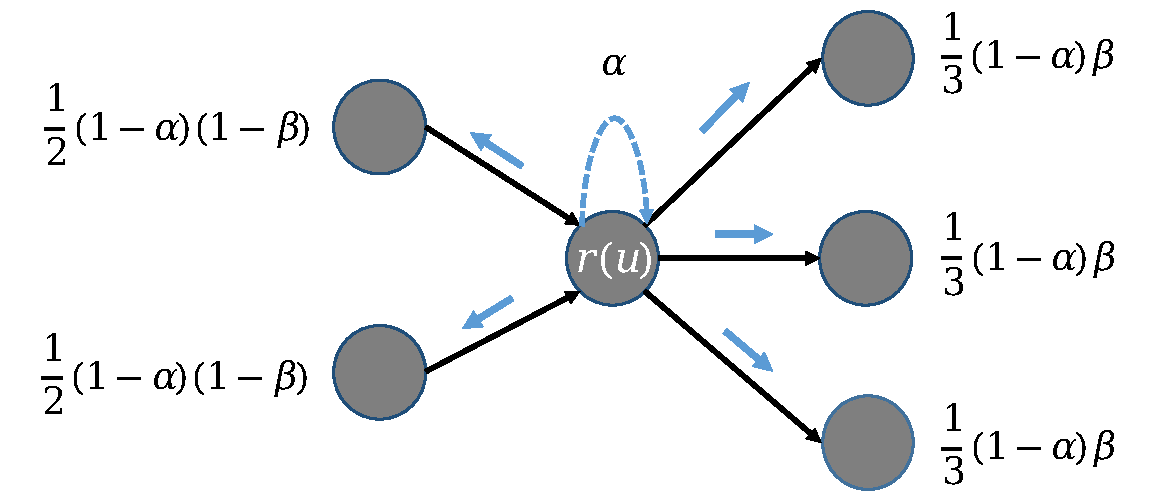
\includegraphics[width=0.3\linewidth]{figures/local_push_ttr_base.pdf}
% %         \label{fig:local_push_ttr_base}
% %     }
% %     \subfigure[weight pollution]{
% %         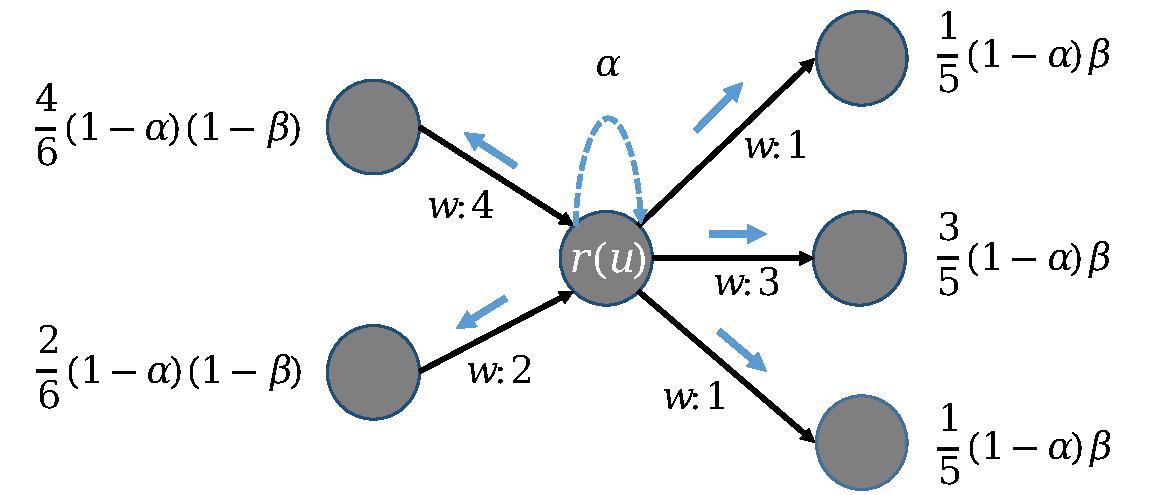
\includegraphics[width=0.3\linewidth]{figures/local_push_ttr_weight.pdf}
% %         \label{fig:local_push_ttr_weight}
% %     }
% %     \subfigure[temporal reasoning]{
% %         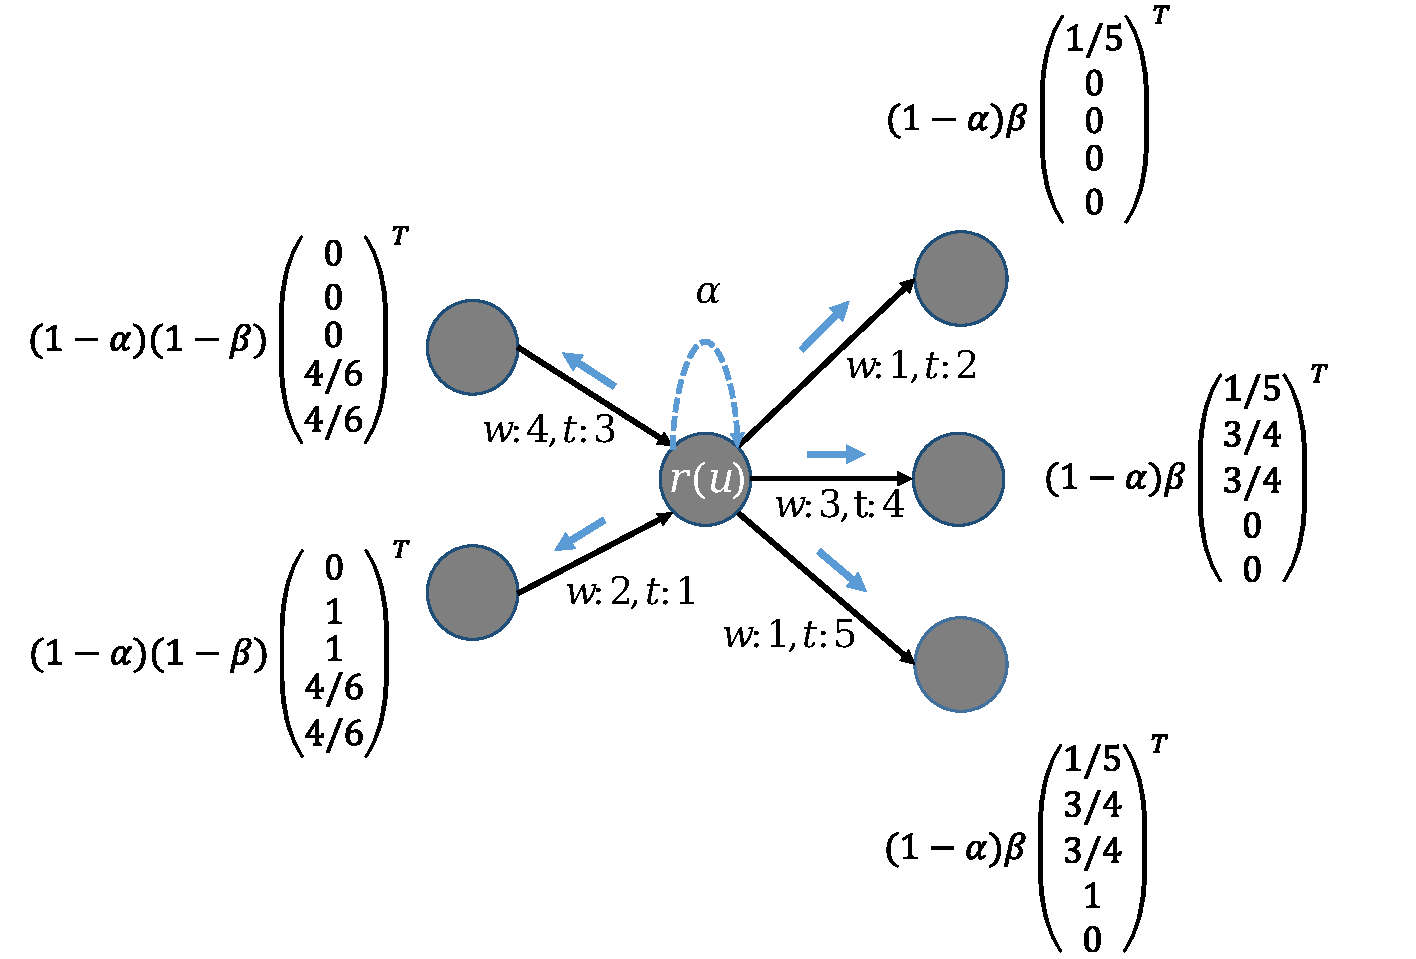
\includegraphics[width=0.3\linewidth]{figures/local_push_ttr_time.pdf}
% %         \label{fig:local_push_ttr_time}
% %     }
% %     \caption{TTR.}
% % \end{figure*}

% % 介绍三种递进的push策略
% \subsubsection{Tracking tendency}
% Since a transaction relationship between addresses is directed, during the transaction tracking process, the attention to in-degree neighbors and out-degree neighbors may be different. 
% For example, tracking for the target of the fund flows oriented from a particular needs to pay more attention to its out-degree neighbors, while searching for the source of money needs to pay more attention to the in-degree neighbors.
% Therefore, considering the transaction network $G$ as a directed graph and giving a tracking tendency coefficient $\beta \in [0,1]$, the out-degree neighbors in a transaction relationship can get a higher estimate of $\bm{p}_s$ when $\beta > 0.5$, and the in-degree neighbors in a transaction relationship can get a higher estimate of $\bm{p}_s$ when $\beta < 0.5$.
% % The local push procedure can push the residual to self, out-degree neighbors, and in-degree neighbors with different ratios.
% In this way, Equation \ref{equ:ppr} can be re-written as:
% \begin{equation}
%     \bm{p}_s = \alpha \bm{e}_s + (1-\alpha) \bm{p}_s M_{\beta}.
%     \label{equ:ttr_base}
% \end{equation}
% The transition matrix of Equation \ref{equ:ttr_base} is:
% \begin{equation}
%     M_{\beta} = \beta D_{out}^{-1}A + (1-\beta)D_{in}^{-1}A^T,
% \end{equation}
% where $A$ is the adjacency matrix of $G$, $D_{out}$ is an out-degree matrix of $G$, and $D_{in}$ is an in-degree matrix of $G$.

% In this way, the local push procedure of node $u$ pushes the residual to itself, out-degree neighbors, and in-degree neighbors. 
% And each in-degree neighbor and each out-degree neighbor receive an equal proportion depending on the in-degree and out-degree, respectively.
% Therefore, Equations \ref{equ:local_push_appr} can be re-written as:
% \begin{equation}
%     \begin{cases}
%         & \bm{p}_s(u)=\bm{p}_s(u)+\alpha \bm{r}_s(u) \\ 
%         & \bm{r}_s(v_{out})=\bm{r}_s(v_{out})+\theta_{\beta}(u,v_{out}) \bm{r}_s(u) \\ 
%         & \bm{r}_s(v_{in})=\bm{r}_s(v_{in})+\theta_{\beta}(u,v_{in}) \bm{r}_s(u)
%     \end{cases},
%     \label{equ:local_push_ttr_base}
% \end{equation}
% where $v_{out} \in N_G^{out}(u)$ and $v_{in} \in N_G^{in}(u)$ denote out-degree neighbor and in-degree neighbor of $u$ respectively, and the push factors are defined as follows:
% \begin{equation}
%     \theta_{\beta}(u,v_{out})=\frac{(1-\alpha)\beta}{d_{out}(u)},
% \end{equation}
% \begin{equation}
%     \theta_{\beta}(u,v_{in})=\frac{(1-\alpha)(1-\beta)}{d_{in}(u)},
% \end{equation}
% in which $d_{out}(u)$ and $d_{in}(u)$ denote out-degree and in-degree of $u$ respectively.
% % \begin{figure}[htb]
% %     \centering
% %     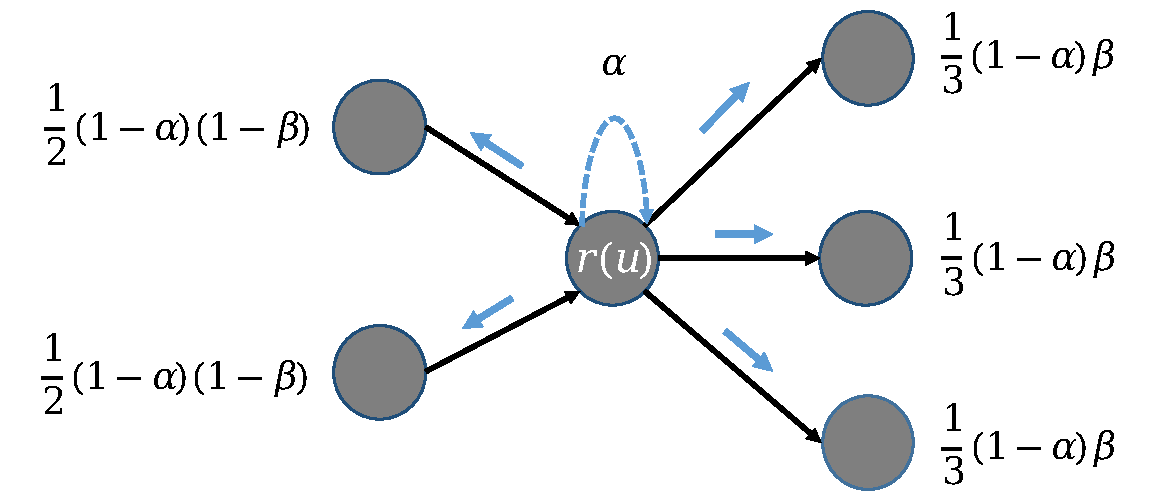
\includegraphics[width=\linewidth]{figures/local_push_ttr_base.pdf}
% %     \caption{Local push procedure with tracking tendency}
% %     \label{fig:local_push_ttr_base}
% % \end{figure}
% And if a node $u$ has no out-degree neighbors or in-degree neighbors, the residual can be pushed to itself.
% % \begin{equation}
% %     r(u)=r(u)+(1-\alpha)\beta r(u),
% % \end{equation}
% % \begin{equation}
% %     r(u)=r(u)+(1-\alpha)(1-\beta) r(u).
% % \end{equation}


% \subsubsection{Weight pollution}
% Traditional APPR pushes the residual of a node to the neighbors by considering an equal weight during a local push iteration. However, in a transaction relationship, the transaction strength is usually weighted by the transaction amount. For each node in the network, a neighbor who has transaction relationships with a larger amount of money is considered to be more relevant to the node. 
% % For example, tracking the fund flow of a node $u$ needs to pay more attention to the neighbors having a large amount of transactions related to $u$.
% % In the procedure of transaction tracking, attention to the nodes whether related to the source node on the amount is needed.
% % For example, the amount received by some nodes is similar to the amount output by the source node, these nodes may be related to the source node.
% Therefore, by considering the transaction network $G$ as a weighted directed graph with the transaction amount information as the weight, Equation \ref{equ:ttr_base} can be re-written as:
% %the nodes get a higher estimate of $\bm{p}_s$ when these nodes have a significant association with the source node on the perspective of edge weight.
% \begin{equation}
%     \bm{p}_s = \alpha \bm{e}_s + (1-\alpha) \bm{p}_s M_w.
%     \label{equ:ttr_weight}
% \end{equation}
% The transition matrix of Equation \ref{equ:ttr_weight} is:
% \begin{equation}
%     % M_w = \beta {D_{out}^w}^{-1}W + (1-\beta){D_{in}^w}^{-1}W^T,
%     M_w = \beta \tilde{D}_{out}^{-1}W + (1-\beta)\tilde{D}_{in}^{-1}W^T,
% \end{equation}
% where $W$ is the weighted adjacency matrix of $G$, $\tilde{D}_{out}$ is the weighted out-degree matrix of $G$, $\tilde{D}_{in}$ is the weighted in-degree matrix of $G$. 
% The diagonal elements of $\tilde{D}_{out}$ and $\tilde{D}_{in}$ are defined as follows:
% \begin{equation}
%     \tilde{D}_{out}(i,i)=||W(i,)||,
% \end{equation}
% \begin{equation}
%     \tilde{D}_{in}(i,i)=||W^T(i,)||, i\leq|V|
% \end{equation}
% where $W(i,)$ and $W^T(i,)$ denote the $i$-th row in $W$ and $W^T$ respectively. All off-diagonal elements in $\tilde{D}_{out}$ and $\tilde{D}_{in}$ equal to 0.

% In this way, the local push procedure of node $u$ pushes residual to itself, the out-degree neighbors and the in-degree neighbors with different ratios determined by edge weight. And Equations \ref{equ:local_push_ttr_base} can be re-written as:
% % \begin{equation}
% %     \begin{cases}
% %       & p(u)=p(u)+\alpha r(u), \\ 
% %       & r(\hat{v})=r(\hat{v})+(1-\alpha)\beta \frac{W(u,\hat{v})}{W(u,)} r(u), \\ 
% %       & r(\tilde{v})=r(\tilde{v})+(1-\alpha)(1-\beta) \frac{W(\tilde{v},u)}{W(,u)} r(u),
% %     \end{cases}
% % \end{equation}
% \begin{equation}
%     \begin{cases}
%       & \bm{p}_s(u)=\bm{p}_s(u)+\alpha \bm{r}_s(u) \\ 
%       & \bm{r}_s(v_{out})=\bm{r}_s(v_{out})+\theta_w(u,v_{out}) \bm{r}_s(u) \\ 
%       & \bm{r}_s(v_{in})=\bm{r}_s(v_{in})+\theta_w(u,v_{in}) \bm{r}_s(u)
%     \end{cases},
%     \label{equ:local_push_weight}
% \end{equation}
% where the push factors are defined as follows:
% \begin{equation}
%     \theta_w(u,v_{out})=(1-\alpha)\beta\frac{w(u,v_{out})}{\tilde{d}_{out}(u)},
% \end{equation}
% \begin{equation}
%     \theta_w(u,v_{in})=(1-\alpha)(1-\beta)\frac{w(v_{in},u)}{\tilde{d}_{in}(u)},
% \end{equation}
% in which $w(u,v)$ for $\forall{u,v \in V}$ denotes the transaction amount from $u$ to $v$, and $\tilde{d}_{out}(u)$ and $\tilde{d}_{in}(u)$ denote the weighted out-degree and weighted in-degree of $u$ respectively.
% % \begin{figure}[htb]
% %     \centering
% %     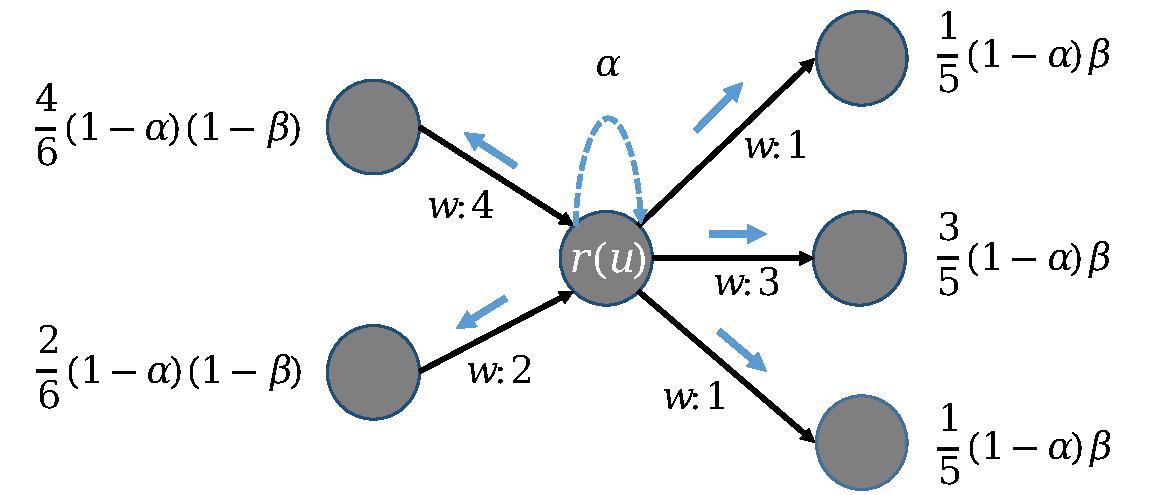
\includegraphics[width=\linewidth]{figures/local_push_ttr_weight.pdf}
% %     \caption{Local push procedure with weight pollution}
% %     \label{fig:local_push_ttr_weight}
% % \end{figure}

% \subsubsection{Temporal reasoning} Blockchain transactions are recorded in blocks chronologically, and each block contains a specific timestamp. Since the fund flow transferring process is dynamic, the transaction time information can be taken into consideration in the local push procedure.
% % Since a transaction relationship is temporal, during the transaction tracking process, the attention to the neighbors may be different.
% In the scenario of blockchain transaction tracking, tracking for the target of a fund flow usually follows the paths with increasing timestamps, while tracking back to the source of a fund flow follows the paths with decreasing timestamps.
% % In the procedure of transaction tracking, starting from the source node, the nodes in the increasing timestamp fund flow or decreasing timestamp fund flow get higher importance.
% % Therefore, considering the transaction network $G$ as a temporal weighted directed graph in which $G^{(t)}$ denotes the weighted directed graph at the $t$-th timestamp, for all timestamp indices $\{1,2, ...,t, ..., t_{\rm max} \}$
% % in $G$, Equation \ref{equ:ttr_weight} can be re-written as:
% Therefore, considering the transaction network $G$ as a temporal weighted directed graph in which $G^{(t)}$ denotes the weighted directed graph at timestamp $t$, for all timestamp $\{ t_1,...,t_k,...,t_n \}$ in $G$, Equation \ref{equ:ttr_weight} can be re-written as:
% \begin{equation}
%     \bm{p}_s^{(t)} = \alpha \bm{e}_s^{(t)} + (1-\alpha) p_s^{(t)} M_w^{(t)},
%     \label{equ:ttr}
% \end{equation}
% where $\bm{p}_s^{(t)}$ denotes the estimate of $\bm{p}_s$ at timestamp $t$, $M_w^{(t)}$ denotes the transition matrix at timestamp $t$, and $\bm{e}_s^{(t)}$ denotes the indicator vector at timestamp $t$ in which $\bm{e}_s^{(t_1)}=\bm{e_s}$ and $\bm{e}_s^{(t_k)} = \bm{p}_s^{(t_{k-1})}$.
% % where $P_s$ is a $t_{max} \times |V|$ matrix in which each row $P_s(t,)$ denotes the importance of all nodes to the source node at $t$-th timestamp.
% % element $\bm{P}_s^{(t)}(u)$ is able to describe the importance of node $u$ to the source node at time $t$
% In this case, $\bm{p}_s$ is redefined as follow:
% \begin{equation}
%     % \bm{p}_s=\sum\limits_{t=1}^{t_{\rm max}}{P_s(t,)}.
%     \bm{p}_s=\frac{1}{n}\sum\limits_{t{'}=t_1}^{t_n}{\bm{p}_s^{(t{'})}}.
% \end{equation}
% % , and the estimate of $p$ can be re-written as $p=\sum_t{p_{\infty}^{(t)}}$.
% The transition matrix of Equation \ref{equ:ttr} is:
% \begin{equation}
%     % M_{t} = \beta \hat{D}_{out}^{-1}W_{t} + (1-\beta)\hat{D}_{in}^{-1}W_{t}^T,
%     % M_{T} = \beta \hat{D}_{out}^{-1}\mathcal{W} + (1-\beta)\hat{D}_{in}^{-1}\mathcal{W}^T,
%     M_{w}^{(t)} = \beta \hat{D}_{out}^{{(t)}^{-1}} W^{(t)} + (1-\beta)\hat{D}_{in}^{{(t)}^{-1}} W^{{(t)}^T},
% \end{equation}
% where $W^{(t)}$ is a weighted adjacency matrix at timestamp $t$, $\hat{D}_{out}^{(t)}$ and $\hat{D}_{in}^{(t)}$ denote the cumulative weighted out-degree matrix and the cumulative weighted in-degree matrix at timestamp $t$ respectively.
% % where $\mathcal{W}$ is a $t_{\rm max} \times |V| \times |V|$ tensor in which $\mathcal{W}(t,)$ denotes the weighted adjacency matrix at the $t$-th timestamp, $\hat{D}_{out}$ and $\hat{D}_{in}$ record the weighted out-degree matrix and the weighted in-degree matrix in each timestamp respectively with the same dimension as $\mathcal{W}$. 
% % $\hat{D}_{out}$ is a temporal weighted out-degree matrix of $G$, 
% % $\hat{D}_{in}$ is a temporal weighted in-degree matrix of $G$, 
% % and $\hat{D}_{out}$ and $\hat{D}_{in}$ have the same dimensions as $W_{t}$.
% The nonzero elements of $\hat{D}_{out}$ and $\hat{D}_{in}$ are defined as follows:
% \begin{equation}
%     % \hat{D}_{out}(t,i,i)=\sum\limits_{t{'}>t}||\mathcal{W}(t',i,)||,
%     \hat{D}_{out}^{(t)}(i,i)=\sum\limits_{t{'}\leq t}||W^{(t{'})}(i,)||,
% \end{equation}
% \begin{equation}
% %   \hat{D}_{in}(t,i,i)=\sum\limits_{t{'}<t}||\mathcal{W}^T(t',i,)||, t\leq t_{\rm max}, i\leq|V|,
%     \hat{D}_{in}^{(t)}(i,i)=\sum\limits_{t{'}\geq t}||W^{(t{'})}(,i)||, t_1 \leq t\leq t_{n}, i\leq|V|,
% \end{equation}
% in which $W^{(t{'})}(i,)$ and $W^{(t{'})}(,i)$ denote the $i$-th row and the $i$-th column in the weighted adjacency matrix at timestamp $t{'}$ respectively.
% % Especially, $\hat{D}_{out}=\tilde{D}_{out}$ and $\hat{D}_{in}=\tilde{D}_{in}$ at timestamp $t_1$.
% % in which $\mathcal{W}(t,i,)$ denotes the row $i$ in the weighted adjacency matrix at the $t$-th timestamp respectively.
% % \begin{equation}
% %     \hat{D}_{t}(i,j,j)=\hat{d}_{t}^{(t_i)}(v_j)=\sum\limits_{t{'}>t}||W_{t}(i,j)||,
% % \end{equation}
% % \begin{equation}
% %   \tilde{D}_{t}(i,j,j)=\tilde{d}_{t}^{(t_i)}(v_j)=\sum\limits_{t{'}<t}||W_{t}^T(i,j)||,
% % \end{equation}
% % in which $W_{t}(i,j)$ and $W_{t}^T(i,j)$ denote the rows $j$ in $W_{t}$ and $W_{t}^T$ at timestamp $t_i$ respectively.

% In this way, the local push procedure of node $u$ pushes the residual to itself, out-degree neighbors, and in-degree neighbors with different ratios determined by the transaction amount and time.
% Equations \ref{equ:local_push_weight} can be re-written as:
% % \begin{equation}
% %     \begin{cases}
% %       & \bm{p}_s(u)=\bm{p}_s(u)+\alpha \bm{e} \cdot R_s(u), \\ 
% %       & R_s(\hat{v})=R_s(\hat{v})+\theta_{t}(u,\hat{v}) \odot R_s(u), \\ 
% %       & R_s(\tilde{v})=R_s(\tilde{v})+\theta_{t}(u,\tilde{v}) \odot R_s(u),
% %     \end{cases}
% % \end{equation}
% \begin{equation}
%     \begin{cases}
%       & \bm{p}_s(u)=\bm{p}_s(u)+\alpha \bm{e} \cdot R_s(u) \\ 
%       & R_s(v_{out})=R_s(v_{out})+\theta_{t}(u,v_{out}) \odot R_s(u) \\ 
%       & R_s(v_{in})=R_s(v_{in})+\theta_{t}(u,v_{in}) \odot R_s(u)
%     \end{cases},
% \end{equation}
% where $R_s$ denotes a $n \times |V|$ matrix in which $R_s(v_i)=R_s(,i)$ denotes the residual of a node $v_i$ at each timestamp, $\odot$ denotes the element-wise product, and the push factors are defined as follows:
% % where $R_s$ denotes a $n \times |V|$ matrix in which $R_s(v_i)=R_s(,i)$ denotes the residual of a node $v_i$ at each timestamp, $\odot$ denotes the element-wise product, and the push factors are defined as follows:
% % \begin{equation}
% %     \theta_{t}(u,\hat{v})=(1-\alpha)\beta w_{t}(u,\hat{v}) \oslash \hat{d}_{t}(u),
% % \end{equation}
% % \begin{equation}
% %     \theta_{t}(u,\tilde{v})=(1-\alpha)(1-\beta) w_{t}(\tilde{v},u) \oslash \tilde{d}_{t}(u),
% % \end{equation}
% \begin{equation}
%     \theta_{t}(u,v_{out})=(1-\alpha)\beta w_{t}(u,v_{out}) \oslash \hat{d}_{out}(u),
% \end{equation}
% \begin{equation}
%     \theta_{t}(u,v_{in})=(1-\alpha)(1-\beta) w_{t}(v_{in},u) \oslash \hat{d}_{in}(u),
% \end{equation}
% in which $w_{t}(u,v)$ for $\forall{u,v \in V}$ is a vector denoting the transaction amount from $u$ to $v$ at each timestamp, $\hat{d}_{out}(u)$ and $\hat{d}_{in}(u)$ denote the temporal weight out-degree and in-degree at each timestamp respectively, and $\oslash$ denotes the element-wise division.

% Based on the above local push strategies, we propose the TTR algorithm.
% Giving a transactions network $G=(V,E)$, TTR tracking for the target starting from the source node $s$.
% Initializing $R_s$ with edges related to $s$, TTR calls the local push procedure to push the residual for a node itself, the out-degree neighbors, and the out-degree neighbors by ``selfPush", ``forwardPush" and ``backwardPush"  procedure respectively, until the residual of each node is within the minimum error $\epsilon$.
% % initializes the estimate $p=\vec{0}$ and the temporal residual $r_{\infty}$, and then 
% % call the local push procedure to push the residual for self, out-degree neighbors and out-degree neighbors by ``selfPush", ``forwardPush" and ``backwardPush"  procedure respectively, until the residual of each node within the minimum error $\epsilon$.
% Algorithm \ref{alg:ttr} describes the framework of the TTR algorithm, Algorithm \ref{alg:self_push}, Algorithm \ref{alg:forward_push} and Algorithm \ref{alg:backward_push} describe the ``selfPush", ``forwardPush" and ``backwardPush" procedure in detail respectively.
% \begin{algorithm}[t]
%     \caption{Transaction Tracking Rank}
%     \label{alg:ttr}
%     \begin{algorithmic}[1]
%         \REQUIRE Source node $s$, transactions network $G=(V,E)$ with timestamp range $\{t_1,t_2,...,t_n\}$, teleport constant $\alpha$, minimum error $\epsilon$, and tracking tendency coefficient $\beta$.
%         \ENSURE the estimate of $\bm{p}_s$
%         \STATE $\bm{p}_s(s)=\alpha$
%         \STATE $R_{s}(t,v)=(1-\alpha)\beta w/\tilde{d}_{out}(s)$ for $\forall{(s,v,w,t)} \in E_{out}(s)$
%         \STATE $R_{s}(t,v)=(1-\alpha)(1-\beta) w/\tilde{d}_{in}(s)$ for $\forall{(v,s,w,t)} \in E_{in}(s)$
%         \IF{$E_{out}(s)=\emptyset$}
%             \STATE $R_s(t_1,s)=(1-\alpha)\beta$
%         \ENDIF
%         \IF{$E_{in}(s)=\emptyset$}
%             \STATE $R_s(t_n,s)=(1-\alpha)(1-\beta)$
%         \ENDIF
%         \WHILE{$||R_s(u)|| \geq \epsilon, u \in V$}
%             \STATE Let $R_s^{\prime}=R_s$, and $R_{s}(u)=\vec{0}$.
%             \STATE Apply $R_s^{\prime}$ to update $\bm{p}_s$ and $R_s$ through selfPush, forwardPush and backwardPush.  
%         \ENDWHILE
%         \RETURN $\bm{p_s}$
%     \end{algorithmic}
% \end{algorithm}

% \begin{algorithm}[t]
%     \caption{selfPush}
%     \label{alg:self_push}
%     \begin{algorithmic}[1]
%         \REQUIRE Node $u$, temporal residual $R_s^{\prime}$, estimate $\bm{p}_s$, and teleport constant $\alpha$.
%         \FOR{$t \in [t_1, t_n]$}
%             \STATE $\bm{p}_s(u)+=\alpha R_s^{\prime}(t,u)$
%         \ENDFOR
%     \end{algorithmic}
% \end{algorithm}

% \begin{algorithm}[t]
%     \caption{forwardPush}
%     \label{alg:forward_push}
%     \begin{algorithmic}[1]
%         \REQUIRE Node $u$, out-edges $E_{out}(u)$, temporal residual $R_s^{\prime}$ and $R_s$, teleport constant $\alpha$, and tracking tendency coefficient $\beta$.
%         \FOR{$\forall{e:(u,v,w,t)} \in E_{out}(u)$}
%             \STATE $\Delta = 0$
%             \FOR{$\tau \in [t_1,t]$}
%                 \STATE $\Delta += w R_s^{\prime}(\tau,u) / \hat{d}_{out}^{(\tau)}(u)$
%                 % \STATE $\Delta += w{\rho}_{\infty}^{(\tau)}(u) / \hat{d}_{\infty}^{(\tau)}(u)$
%             \ENDFOR
%             % \STATE $r^{(t)}_{\infty}(\hat{v})+=(1-\alpha) \beta \Delta$
%             \STATE $R_s(t,v) += (1-\alpha)\beta \Delta$
%         \ENDFOR
%         \STATE Calculate $max(t)$ from all $t$ in $E_{out}(u)$.
%         \FOR{$\tau \in [max_t, t_n]$}
%             % \STATE $r_{\infty}^{(\tau)}(u)+=(1-\alpha)\beta {\rho}_{\infty}^{(\tau)}(u)$
%             \STATE $R_s(\tau,u) += (1-\alpha)\beta R_s^{\prime}(\tau,u)$
%         \ENDFOR
%     \end{algorithmic}
% \end{algorithm}

% \begin{algorithm}[t]
%     \caption{backwardPush}
%     \label{alg:backward_push}
%     \begin{algorithmic}[1]
%         \REQUIRE Node $u$, in-edges $E_{in}(u)$, temporal residual $R_s^{\prime}$ and $R_s$, teleport constant $\alpha$, and tracking tendency coefficient $\beta$.
%         \FOR{$\forall e:(v,u,w,t) \in E_{in}(u)$}
%             \STATE $\Delta = 0$
%             \FOR{$\tau \in [t, t_n]$}
%                 % \STATE $\Delta += w{\rho}_{\infty}^{(\tau)}(u) / \tilde{d}_{\infty}^{(\tau)}(u)$
%                 \STATE $\Delta += w R_s^{\prime}(\tau, u) / \hat{d}_{in}^{(\tau)}(u)$
%             \ENDFOR
%             % \STATE $r_{\infty}^{(t)}(\tilde{v}) += (1-\alpha)(1-\beta)\Delta$
%             \STATE $R_s(t,v) += (1-\alpha)(1-\beta)\Delta$
%         \ENDFOR
%         \STATE Calculate $min(t)$ from all $t$ in $E_{in}(u)$.
%         \FOR{$\tau \in [t_1, min(t)]$}
%             % \STATE $r_{\infty}^{(\tau)}(u)+=(1-\alpha)(1-\beta) {\rho}_{\infty}^{(\tau)}(u)$
%             \STATE $R_s(\tau,u)+=(1-\alpha)(1-\beta) R_s^{\prime}(\tau,u)$
%         \ENDFOR
%     \end{algorithmic}
% \end{algorithm}

% % \begin{algorithm}[htb]
% %     \caption{forwardPush}
% %     \label{alg:forward_push}
% %     \begin{algorithmic}[1]
% %         \REQUIRE node $u$, out-edges set of node $E(u,)$, residual vector $r$, tracking tendency coefficient $\alpha$ and $\beta$.
% %         \STATE // sort $E(u,)$ and $r(u)$ by timestamp increasingly
% %         \STATE $E(u,)=sort(E(u,))$ 
% %         \STATE $r(u)=sort(r(u))$

% %         \STATE // calcuate sum of weight after each chips
% %         \STATE $j=|E(u,)|-1,w=0,W=mapping$
% %         \FOR{$i \in |r(u)|,|r(u)|-1,...,0$}
% %             \STATE $c=r(u)^i$
% %             \WHILE{$j \geq 0 \wedge E(u,)_t^j > c_t$}
% %                 \STATE $w = w + E(u,)_w^j$
% %                 \STATE $j = j - 1$
% %             \ENDWHILE
% %             \STATE $W(c)=w$
% %         \ENDFOR
        
% %         \STATE // propagate residual weight to outdegree heighbors
% %         \STATE $j=0,d=0$
% %         \FOR{$i \in 0,1,...,|E(u,)|$}
% %             \STATE $e=E(u,)^i$
% %             \WHILE{$j < |r(u)| \wedge e_t > r(u)_t^j$}
% %                 \IF{$W(r(u)^j) > 0$}
% %                     \STATE $d = d + \frac{r(u)_w^j}{W(r(u)^j)}$
% %                 \ENDIF
% %                 \STATE $j = j + 1$
% %                 \STATE $r(e_v)_t=r(e_v)_t + (1-\alpha)\beta e_w d$
% %             \ENDWHILE
% %         \ENDFOR
        
% %         \STATE // not propagated residual weight will back to node $u$
% %         \WHILE{$ j < |r(u)| $}
% %             \STATE $r(u) = r(u) \cup (r(u)_t^j, (1-\alpha)\beta r(u)_w^j)$
% %             \STATE $j=j+1$
% %         \ENDWHILE
% %     \end{algorithmic}
% % \end{algorithm}

% % \begin{algorithm}[htb]
% %     \caption{backwardPush}
% %     \label{alg:backward_push}
% %     \begin{algorithmic}[1]
% %         \REQUIRE node $u$, in-edges set of node $E(,u)$, residual vector $r$, tracking tendency coefficient $\alpha$ and $\beta$.
% %         \STATE // sort $E(,u)$ and $r(u)$ by timestamp increasingly
% %         \STATE $E(,u)=sort(E(,u))$ 
% %         \STATE $r(u)=sort(r(u))$

% %         \STATE // calcuate sum of weight after each chips
% %         \STATE $j=0,w=0,W=mapping$
% %         \FOR{$i \in 0,1,...,|r(u)|$}
% %             \STATE $c=r(u)^i$
% %             \WHILE{$j < |E(,u)| \wedge E(,u)_t^j < c_t$}
% %                 \STATE $w = w + E(,u)_w^j$
% %                 \STATE $j = j + 1$
% %             \ENDWHILE
% %             \STATE $W(c)=w$
% %         \ENDFOR
        
% %         \STATE // propagate residual weight to indegree heighbors
% %         \STATE $j=|r(u)|-1,d=0$
% %         \FOR{$i \in |E(,u)|,|E(,u)|-1,...,0$}
% %             \STATE $e=E(u)^i$
% %             \WHILE{$j \geq 0 \wedge e_t < r(u)_t^j$}
% %                 \IF{$W(r(u)^j) > 0$}
% %                     \STATE $d = d + \frac{r(u)_w^j}{W(r(u)^j)}$
% %                 \ENDIF
% %                 \STATE $j = j - 1$
% %                 \STATE $r(e_v)_t=r(e_v)_t + (1-\alpha)(1-\beta) e_w d$
% %             \ENDWHILE
% %         \ENDFOR
        
% %         \STATE // not propagated residual weight will back to node $u$
% %         \WHILE{$ j \geq 0 $}
% %             \STATE $r(u) = r(u) \cup (r(u)_t^j, (1-\alpha)(1-\beta) r(u)_w^j)$
% %             \STATE $j=j-1$
% %         \ENDWHILE
% %     \end{algorithmic}
% % \end{algorithm}

% Here are some useful theorems (also see \cite{andersen2006local}) to describe the cost of TTR algorithm, and the proofs  given in appendices. 

% \begin{theorem}
% \label{thm:run_time}
% Line 10-line 13 in Algorithm \ref{alg:ttr}, runs in $O(\frac{1}{\epsilon \alpha})$ time, and the number of nodes with non-zero values in the output TTR vector is at most $O(\frac{1}{\epsilon \alpha})$.
% \end{theorem}


% \begin{theorem}
% \label{thm:push_cost}
% The cost of local push procedure including selfPush, forwardPush and backwardPush is $O(|E(u)|log(|E(u)|)$.
% \end{theorem}


% \subsection{TTR-based Push-Pop Model}
% The TTR-based Push-Pop model uses the TTR algorithm as the transaction tracking strategy, which can track the fund flow of the source node $s$ in a transaction network, calculate the relevance between other nodes in the network and the source node, and output a local tracking network.

% For initialization, the TTR-based Push-Pop model set $V_s^T=\{s\}$, and then calls \textit{pop}, \textit{expand}, and \textit{push} in turns until $||R_s(u)|| < \epsilon$ for $\forall{u \in V_s^T}$.
% Finally, the TTR-based Push-Pop model calls \textit{extract} for outputting a local tracking network.
% % The TTR-based Push-Pop model can be described as Algorithm \ref{alg:ttr_based_push_pop}, and
% % where the TTR Strategy maintains all parameters of TTR Algorithm \ref{alg:ttr} like $\epsilon$, and the witnessed graph $G_T=(V_T, E_T)$.
% % the witnessed nodes $V_T$, and the witnessed edges $E_T$.
% The procedures of the TTR strategy in TTR-based Push-Pop model are as follows:
% \begin{itemize}
%     \item \textit{expand}: Query the related edges for a given node $u$. 
%     % Refer to line 4 of Algorithm \ref{alg:ttr_based_push_pop}.
%     \item \textit{push}: The TTR strategy receives a series of edges related to a node $u$ for updating the witnessed network $G_s^T$, and calls the local push procedure for $u$. 
%     % Refer to line 5 of Algorithm \ref{alg:ttr_based_push_pop}.
%     \item \textit{pop}: Output a node that has a maximum residual from $V_s^T$. 
%     % Refer to line 3 of Algorithm \ref{alg:ttr_based_push_pop}.
%     \item \textit{extract}: Output a local tracking network through the TTR-based Local Community Discovery Algorithm \ref{alg:ttr_based_local_comm}. 
%     % Refer to line 7 of Algorithm \ref{alg:ttr_based_push_pop}.
% \end{itemize}

% % \begin{algorithm}[htb]
% %     \caption{TTR-based Push-Pop Model}
% %     \label{alg:ttr_based_push_pop}
% %     \begin{algorithmic}[1]
% %         \REQUIRE the source node $s$, transaction network $G$, TTR Strategy $T$
% %         \ENSURE a local tracking network captured by $T$
% %         \STATE $T.init(s)$
% %         \WHILE{$max(||R_s(u)||) \geq \epsilon, u \in V_T$}
% %             \STATE $u = T.maxResidualNode()$
% %             \STATE $E(u) = T.query(G,u)$
% %             \STATE $T.localPush(E(u))$
% %         \ENDWHILE
% %         \RETURN $T.localComm()$
% %     \end{algorithmic}
% % \end{algorithm}

% Aiming at extracting the most important partition of $G_s^T$, the TTR-based Local Community Discovery Algorithm \ref{alg:ttr_based_local_comm} constructs a local community as the local tracking network.
% Here, we define a subgraph $G_{sub}$ of $G_s^T$ with a low conductance as the local community according to previous work \cite{andersen2006local, andersen2007local}, in which its conductance is:
% \begin{equation}
% \Phi(S)=\frac{\bm{p}_s(\partial(S))}{\bm{p}_s(S)}
% \end{equation}
% where $S \subseteq V_s^T$ denotes the nodes of $G_{sub}$, the boundary $\partial(S)=\{ v| (u,v) \in E_t \land u \in S \land v \in \bar{S} \}$, $\bar{S}$ is the complement of $S$ and $\bm{p}_s(S)=\sum_{u \in S}\bm{p}_s(u)$ denotes the sum of $\bm{p}_s$ over each node in $S$.
% % In fact, raw local tracking network contains lots of redundant information, such as nodes and edges without highly related to the source node. 
% % For this reason, this section will proposes the TTR-based local community discovery algorithm to extract the most important partition of the raw local tracking network.
% % Giving a nodes set $S$ of partition, the conductance of this partition $\Phi(S)$ satisfies:
% In this way, a subgraph $G_{sub}$ of $G_s^T$ is a local community satisfying:
% \begin{equation}
%     \Phi(S) < \varphi,
%     \label{equ:ttr_local_comm_end_cond}
% \end{equation}
% where $\varphi$ denotes the maximum conductance of $S$.
% For initialization, algorithm \ref{alg:ttr_based_local_comm} set $S=\{s\}$, and then adds a node with the maximum estimate of $\bm{p}_s$ in \textcolor{red}{$V_s^T$} on each step until satisfying Equation \ref{equ:ttr_local_comm_end_cond}.
% \begin{algorithm}[t]
%     \caption{TTR-based Local Community Discovery}
%     \label{alg:ttr_based_local_comm}
%     \begin{algorithmic}[1]
%         \REQUIRE The source node $s$, the witnessed network $G_s^T=(V_s^T, E_s^T)$
%         \ENSURE the local tracking network
%         \STATE $S = \{ s \}$
%         \STATE $\bm{p}_s = TransactionTrackingRank(s,G_s^T,\epsilon,\alpha,\beta)$
%         \WHILE{$\Phi(S) \geq \varphi$}
%             \STATE $u = maxEstimateNode(\bm{p}_s)$
%             \STATE $S = S \cup \{ u \}$
%         \ENDWHILE
%         \RETURN $G_s^T.subgraph(S)$
%     \end{algorithmic}
% \end{algorithm}

% Here are two properties of the TTR-based Push-Pop model and their proofs are given in appendices.

% \begin{proposition}
% \label{pot:ttr_max_height}
% A $n$-order neighbor \cite{lin2020modeling} of the source node can be found in \textcolor{red}{$V_s^T$}, in which $n$ satisfies:
% \begin{equation}
%     n \leq \frac{log(\epsilon)}{log(1-\alpha)}.
% \end{equation}

% This proposition estimates what depth can the TTR-based Push-Pop model track in a network from the source node.
% \end{proposition}

% \begin{proposition}
% \label{pot:ttr_local_comm}
% At least one path between the source node $s$ and a $n$-order target node $v_n$ can be found in local tracking network of TTR-based Push-Pop model under the worst conditions, which requires:
% \begin{equation}
%     \begin{cases}
%         & \varphi \geq \epsilon \\
%         & \bar{d}\varphi^{\frac{1}{n}} \leq (1-\alpha) \cdot min(\beta,1-\beta) 
%     \end{cases},
% \end{equation}
% where $\bar{d}$ denotes the average degree of nodes in the paths among the source node and target nodes.
% \end{proposition}

% Let $n$ denotes the nodes number of a local transaction network, we suggest that $\epsilon=\Omega (\frac{1}{n})$ \cite{zhang2016approximate}. 
% % because a node with $\bm{p}_s$ in which each element is less than $\frac{1}{n}$ is meaningless 
% The proposition \ref{pot:ttr_local_comm} limits the value range of 
% each parameter in Algorithm \ref{alg:ttr_based_local_comm}.
\section{Experiments}
\label{sec:experiments}
In this section, we conduct experiments to evaluate the effectiveness of TRacer on a large-scale real-world dataset. Besides, we conduct case studies with network visualization techniques.

\subsection{Experimental Setups}
% 主要包括参数设置、数据集描述、指标、对比算法

\subsubsection{Dataset}
We contribute a benchmark dataset including 20 transaction tracing cases in the recent 5 years across three account-based blockchains, i.e., Ethereum, Binance Smart Chain, and Polygon. 
These cases are initialized by various illegal activities containing hacker attacks, Rug-pull, and scams which have caused billions of dollars in losses. 
All these cases are reported by blockchain security companies and verified by experts coming from Certik \footnote{https://www.certik.com/}, Peckchield \footnote{https://peckshield.com/}, Chainalysis \footnote{https://www.chainalysis.com/} and so on.
Some statistics of this dataset are shown in Table \ref{tab:dataset}. 
Note that the transaction data in the dataset is obtained from the open APIs\footnote{https://blockscan.com}.
As we can see, the activities of these cases have acrossed millions of blocks, and we have to trace the money flows of the sources among more than 4 billion transactions.

\begin{table}[t]
  \caption{Statistics of the transaction record data related to the cases }
  \label{tab:dataset}
  \begin{tabular}{l|l|l}
    \hline
    \textbf{Field} & \textbf{Description} & \textbf{Number} \\
    \hline
    Source nodes & \tabincell{l}{The source node related to this\\case, such as the hacker account\\ and the scam contract.} & 20 \\ \hline
    Target nodes & \tabincell{l}{A set of target nodes related to\\this case, such as exchange\\wallets and mixing services.}  & 0.87K \\ \hline
    Blocks & \tabincell{l}{The blocks related to these cases.}  & 23.5M \\ \hline
    Transactions & \tabincell{l}{The transactions contained in the\\blocks related to these cases.} & 4.83B \\ \hline
  \end{tabular}
\end{table}
% Experiments are started from the source node in these cases in order to find the target nodes.

% \begin{table}[t]
%     \caption{Statistics of Cases}
%     \centering
%     \begin{threeparttable}
%         \begin{tabular}{cccccc}
%             \hline
%             Case & Source\tnote{1} & \#Target & \#Node & \#Edge & Block\tnote{2}\\
%             \hline
%             PlusToken & 0xf4a2e & 17 & 68 & 164 & 7993213\\
%             TokenStore & 0x068ac & 5 & 80 & 194 & 7802134\\
%             Cryptopia & 0xd4e79 & 4 & 9 & 24 & 9128188\\
%             Kucoin & 0xeb319 & - & - & - & 10933499\\
%             Upbit & 0xa0987 & - & - & - & 9007863\\
%             \hline
%         \end{tabular}
%         \begin{tablenotes}    
%             \footnotesize              
%             \item[1] Here provides the address prefix of the source node.
%             \item[2] Here provides the block number of the first transaction related to the cases.
%         \end{tablenotes}  
%     \end{threeparttable}
%     \label{tab:cases}
% \end{table}

% \begin{table*}[htb]
%     \caption{Experimental Results.}
%     \centering
%     \begin{threeparttable}
%         \begin{tabular}{cccccccccccccccc}
%             \hline
%              & \multicolumn{3}{c}{PlusToken} & \multicolumn{3}{c}{TokenStore} & \multicolumn{3}{c}{Cryptopia} & \multicolumn{3}{c}{Kucoin} & \multicolumn{3}{c}{Upbit} \\ \cmidrule(r){2-4} \cmidrule(r){5-7} \cmidrule(r){8-10} \cmidrule(r){11-13} \cmidrule(r){14-16}
%             Methods & $D_l$ & $K$ & $R$ & $D_l$ & $K$ & $R$ & $D_l$ & $K$ & $R$ & $D_l$ & $K$ & $P_l$ & $D_l$ & $K$ & $P_l$\\ \hline
%             BFS & 4.0$\times 10^{-9}$ & 3 & \textbf{0.93} &
%                 1.6$\times 10^{-7}$ & 3 & 0.4 &
%                 3.4$\times 10^{-7}$ & 3 & 1.0 &
%                 1.1$\times 10^{-8}$ & 3 & - &
%                 3.8$\times 10^{-9}$ & 3 & -\\
%             Poison & 6.3$\times 10^{-9}$ & 3 & 0 &
%                 1.6$\times 10^{-7}$ & 3 & 0.4 &
%                 2.3$\times 10^{-6}$ & 3 & 1.0 &
%                 2.3$\times 10^{-8}$ & 3 & - &
%                 6.4$\times 10^{-6}$ & 3 & -\\
%             Haircut & 7.6$\times 10^{-9}$ & \textbf{6} & \textbf{0.93} &
%                 8.1$\times 10^{-8}$ & \textbf{6} & \textbf{1.0} &
%                 7.0$\times 10^{-8}$ & 7 & \textbf{1.0}\tnote{*} &
%                 2.0$\times 10^{-5}$ & 4 & - &
%                 4.0$\times 10^{-7}$ & 5 & -\\
%             APPR & 0 & 0 & 0 &
%                 8.1$\times 10^{-4}$ & 5 & 0.4 &
%                 3.1$\times 10^{-4}$ & 7 & \textbf{1.0}\tnote{*} &
%                 6.0$\times 10^{-4}$ & 4 & 0.25 &
%                 2.4$\times 10^{-4}$ & 4 & 0.26\\
%             \hline
%             TTR-base & 4.9$\times 10^{-5}$ & 5 & \textbf{0.93} & 
%                 \textbf{2.0}\bm{$\times$}\textbf{10}$^{-3}$ & 5 & 0.4 & 
%                 4.0$\times 10^{-4}$ & 6 & \textbf{1.0}\tnote{*} & 
%                 \textbf{6.2}\bm{$\times$}\textbf{10}$^{-4}$ & 4 & 0.26 & 
%                 2.8$\times 10^{-4}$ & 6 & 0.44\\
%             TTR-weight & 2.2$\times 10^{-5}$ & \textbf{6} & \textbf{0.93} & 
%                 2.8$\times 10^{-4}$ & \textbf{6} & \textbf{1.0} & 
%                 6.9$\times 10^{-4}$ & 7 & \textbf{1.0}\tnote{*} & 
%                 2.7$\times 10^{-4}$ & 5 & 0.39 & 
%                 4.0$\times 10^{-4}$ & \textbf{8} & \textbf{0.75}\\
%             TTR-time & \textbf{1.2}\bm{$\times$}\textbf{10}$^{-4}$ & 5 & \textbf{0.93} &
%                 1.6$\times 10^{-4}$ & \textbf{6} & \textbf{1.0} &
%                 \textbf{9.6}\bm$\times$\textbf{10}$^{-4}$ & \textbf{10} & \textbf{1.0}\tnote{*} &
%                 2.2$\times 10^{-4}$ & \textbf{7} & \textbf{0.52} & 
%                 \textbf{4.3}\bm$\times$\textbf{10}$^{-4}$ & \textbf{8} & 0.65\\
%              \hline
%         \end{tabular}
%         \begin{tablenotes}    
%             \footnotesize              
%             \item[*] These methods can find some extra suspicious target nodes, referring to Section \ref{sec:case_study_Cryptopia}.
%         \end{tablenotes}
%     \end{threeparttable}
%     \label{tab:experimentations}
% \end{table*}

\subsubsection{Compared Methods}
We compare our method with several baseline blockchain transaction tracing methods. For a fair comparison, we use the general framework of TRacer to reproduce the following comparison methods, including:
\begin{itemize}
    \item \textbf{BFS} \cite{zhao2015graph}: Breadth-First Search, which is the first and the most commonly used transaction tracing method.
    \item \textbf{Poison} \cite{moser2014towards}: A kind of taint analysis technology in blockchain transaction tracing. Each output of a transaction with a dirty input is considered to be tainted in this method.
    \item \textbf{Haircut} \cite{moser2014towards}: A kind of taint analysis technology in blockchain transaction tracing. Each output of a transaction with a dirty input is considered to be tainted partially according to the amount value in this method. 
    \item \textbf{APPR} \cite{andersen2006local}: The approximate personalized PageRank algorithms, which can calculate the relevance of nodes in a network to a given source node with an extremely low cost.
    % \item \textbf{TRacer}: The method we proposed, where the graph construction recognizes the transaction patterns, the TTR and greedy selection are used for graph expansion, and the local community detection is applied in Extract.
    % using a novel local push procedure, and we abbreviate the TTR algorithm with tracing tendency, weight pollution, and temporal reasoning strategies as TTR-base, TTR-weight, and TTR-time respectively.
\end{itemize}

The details of implementing the above transaction tracing technologies can be found in our GitHub page \footnote{https://github.com/wuzhy1ng/BlockchainSpider}.

\subsubsection{Experimental Settings} 
% {\color{blue}Based on the experiences, it is enough for BFS and Poison to trace the 2-order neighbors of the source node, since the increase of order leads to the exponential growth of the size of subgraph in graph expansion for these two methods, bringing great difficulty to transaction auditing.}
%%  !!!! 这段话大有问题
Since the increase of depth can lead to the exponential growth of the size of output graph in BFS and Poison, bringing great difficulty to transaction auditing. During our experiments, we set the upper limit of the tracing depth in these two methods is 2. In addition, we use the Haircut method to trace the ``dirty money'' from the source node until the amount proportion of ``dirty money" of all nodes is less than 0.1\% of that from the source node.
Moreover, we set $\alpha=0.15$, $\epsilon=10^{-3}$ for APPR and TTR, and $\varphi=10^{-3}$, $\beta=0.7$ for TTR to ensure that our method is able to find the paths among the source node and the target nodes with 42-hop at most, according to Proposition \ref{pot:max_depth}.

\subsubsection{Metrics}
we report the average of the following metrics in all cases to measure the effectiveness of transaction tracing:
% We use the following metrics to measure the effectiveness of transaction tracing:
\begin{itemize}
    \item \textbf{Recall}: The recall evaluates how many target nodes can be traced by a method, which is defined as: $Recall = \frac{|V_t|}{|\bar{V_t}|}$, where $|V_t|$ is the number of traced target nodes and $|\bar{V_t}|$ is the number of all target nodes in a case.
    
    \item \textbf{Number of nodes}: This metric measures the number of nodes in the output graph of a case. A smaller output graph with recall ensured is easier for expert auditing.
    % Ensuring the recall, the fewer node number, the more conducive to expert verification.
    
    \item \textbf{Tracing depth}: This metric measures how deep can a transaction tracing method traverse the transaction graph from a source node, indicating that up to $K$-hop neighbors of the source node are detected.
\end{itemize}

\subsection{Experimental Results}
% 参数敏感性实验
\subsubsection{Scalability vs. Performance}
\begin{figure}[t]
    \centering
    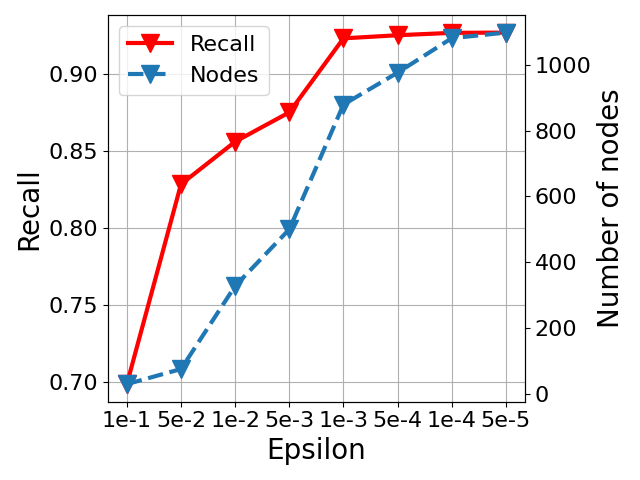
\includegraphics[width=0.65\linewidth,height=3.7cm]{figures/epsilon_metrics.png}
    \vskip -0.1in
    \caption{The relationship among Epsilon, Recall, and Node number. Note that the recall has reached 70\% with $\epsilon = 10^{-1}$ merely, and the increment of recall becomes slow when $\epsilon$ is less than $10^{-3}$.}
    \label{fig:epsilon_metrics}
\end{figure}
The approximation parameter $\epsilon$ is an important hyper-parameters in modulating the scalability.
To examine the effect of $\epsilon$ on the performance, we repeat experiments with different values of $\epsilon$ and report the recall as well as the number of traced nodes. 
As Figure \ref{fig:epsilon_metrics} shows, the recall has reached 70\% when $\epsilon = 10^{-1}$.
When $\epsilon$ is less than $10^{-3}$, the increment of recall becomes slow, and the number of nodes rapidly increases. 
Therefore, setting $\epsilon = 10^{-3}$ can guarantee a higher recall and fewer nodes with a relatively low cost in experiments, and we set $\epsilon = 10^{-3}$ for TRacer.
% , which is the reason why we set $\epsilon = 10^{-3}$ for TRacer.


% 对比实验
\subsubsection{Comparative experiment}
\begin{table}[t]
  \caption{
  Performance comparison between baselines and TRacer
%   Comparative experiment results. Besides the number of tracing nodes being more than APPR slightly, the recall and tracing depth are better than other methods significantly.
  }
  \label{tab:compared_methods}
  \begin{tabular}{cccc}
    \toprule
    Methods & Recall (\%) & Number of nodes (K) & Tracing depth\\
    \midrule
    BFS & 77.02 & 52.50 & 2.00\\
    Poison & 70.06 & 41.45 & 2.00\\
    Haircut & 58.85 & 10.35 & 4.15\\
    APPR & 71.92 & \textbf{0.66} & 3.60\\
    \textbf{TRacer} & \textbf{92.31} & 0.87 & \textbf{5.05}\\
  \bottomrule
\end{tabular}
\end{table}
Table \ref{tab:compared_methods} shows the performance of different methods, from which we can obtain the following observations.
\textbf{\textit{Firstly}}, the output graphs of BFS and Poison contain an extremely large number of nodes, which brings great difficulty to transaction auditing even through detecting more than 70\% target nodes.
\textbf{\textit{Secondly}}, the output graph of Haircut has fewer nodes than BFS and Poison with a greater tracing depth, but the recall is too low to achieve effective tracing.
\textbf{\textit{Thirdly}}, fewest nodes are obtained by APPR, ensuring the detection results can be easier audited by experts. 
\textbf{Fourthly}, TRacer obtains better performance than APPR. On the basis of the advantages of APPR, the recall and tracing depth of TRacer are significantly better than other methods.

% 消融实验
\subsubsection{Ablation experiment}
\begin{table}[t]
  \caption{Ablation experiment.}
  \label{tab:ablation_experiment}
  \setlength{\tabcolsep}{0.1mm}{
  \begin{tabular}{p{2.5cm}<{\centering}p{1.4cm}<{\centering}p{2.2cm}<{\centering}|p{0.6cm}<{\centering}p{1.8cm}<{\centering}}
    \toprule
    Graph construction with DeFi patterns & Graph expansion & Local community detection & Recall (\%) & Number of nodes (K)\\
    % pattern recognition & expansion & detection & (\%) & of nodes (K)\\
    \midrule
    $\surd$ & $\surd$ & $\surd$ & 92.3 & 0.87\\
     & $\surd$ & $\surd$ & 80.3 & 0.55\\
    $\surd$ & $\surd$ &  & 95.9 & 57.5\\
  \bottomrule
\end{tabular}}
\end{table}
TRacer is consist of three modules including graph construction, graph expansion, and local community detection. 
In order to discuss the function of different modules, we conduct an ablation study and report the performance of TRacer in Table \ref{tab:ablation_experiment} after removing the DeFi pattern recognition in graph construction and the local community detection.
% remove the graph construction module recognizing the edge patterns or local community detection module extracting the important local community, and report the performance as shown in Table \ref{tab:ablation_experiment}.
When the DeFi pattern recognition is removed in the graph construction module, the recall decreases significantly, which shows that the understanding of DeFi patterns in TRacer can help trace the money flows effectively.
Moreover, if the local community detection module is removed, the number of nodes increases significantly with the weakly improvement of recall, which shows that the local community detection module can find the nodes strongly associated with the source node at the cost of a small recall loss.

% Top N recall
\subsubsection{Top\textit{N} Recall}
\begin{figure}[t]
    \centering
    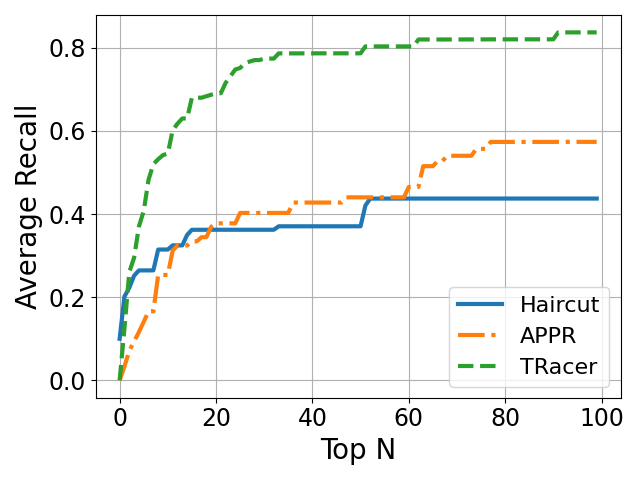
\includegraphics[width=0.6\linewidth]{figures/topn_recall_v2.png}
    \caption{Top $n$ most relevant nodes and the recall. 
    % TRacer tends to give higher importance to the target nodes.
    }
    \label{fig:topn_recall}
\end{figure}

Since the rank of a node represents the relevance relationship between this node and the source node, we can audit the nodes according to the descending order of rank. To compare the rank-based methods including Haircut, APPR, and TRacer, we take out the top $n$ most relevant nodes to the source and calculate the recall for different $n$.
The result is displayed in Figure \ref{fig:topn_recall}, where the curve of TRacer shows a better performance than other methods.
In addition, TRacer achieves a 25\% recall gain over APPR when $n>50$.

\subsection{Case Study}
\label{sec:case_study}
% 该部分对案例中的TTR局部交易网络进行分析
% In this part, we visualize the fund flow on cases with verified labels by Gephi 0.9.2 \cite{bastian2009gephi}.
In this part, we visualize the traced money flow of two cases with Gephi 0.9.2 \cite{bastian2009gephi}, in order to evaluate the feasibility of TRacer.
% In this section, we give the analysis of cases with the local tracing network captured by our method through gephi.

\subsubsection{Cryptopia}\label{sec:case_study_Cryptopia}
\begin{figure}[t]
    \centering
    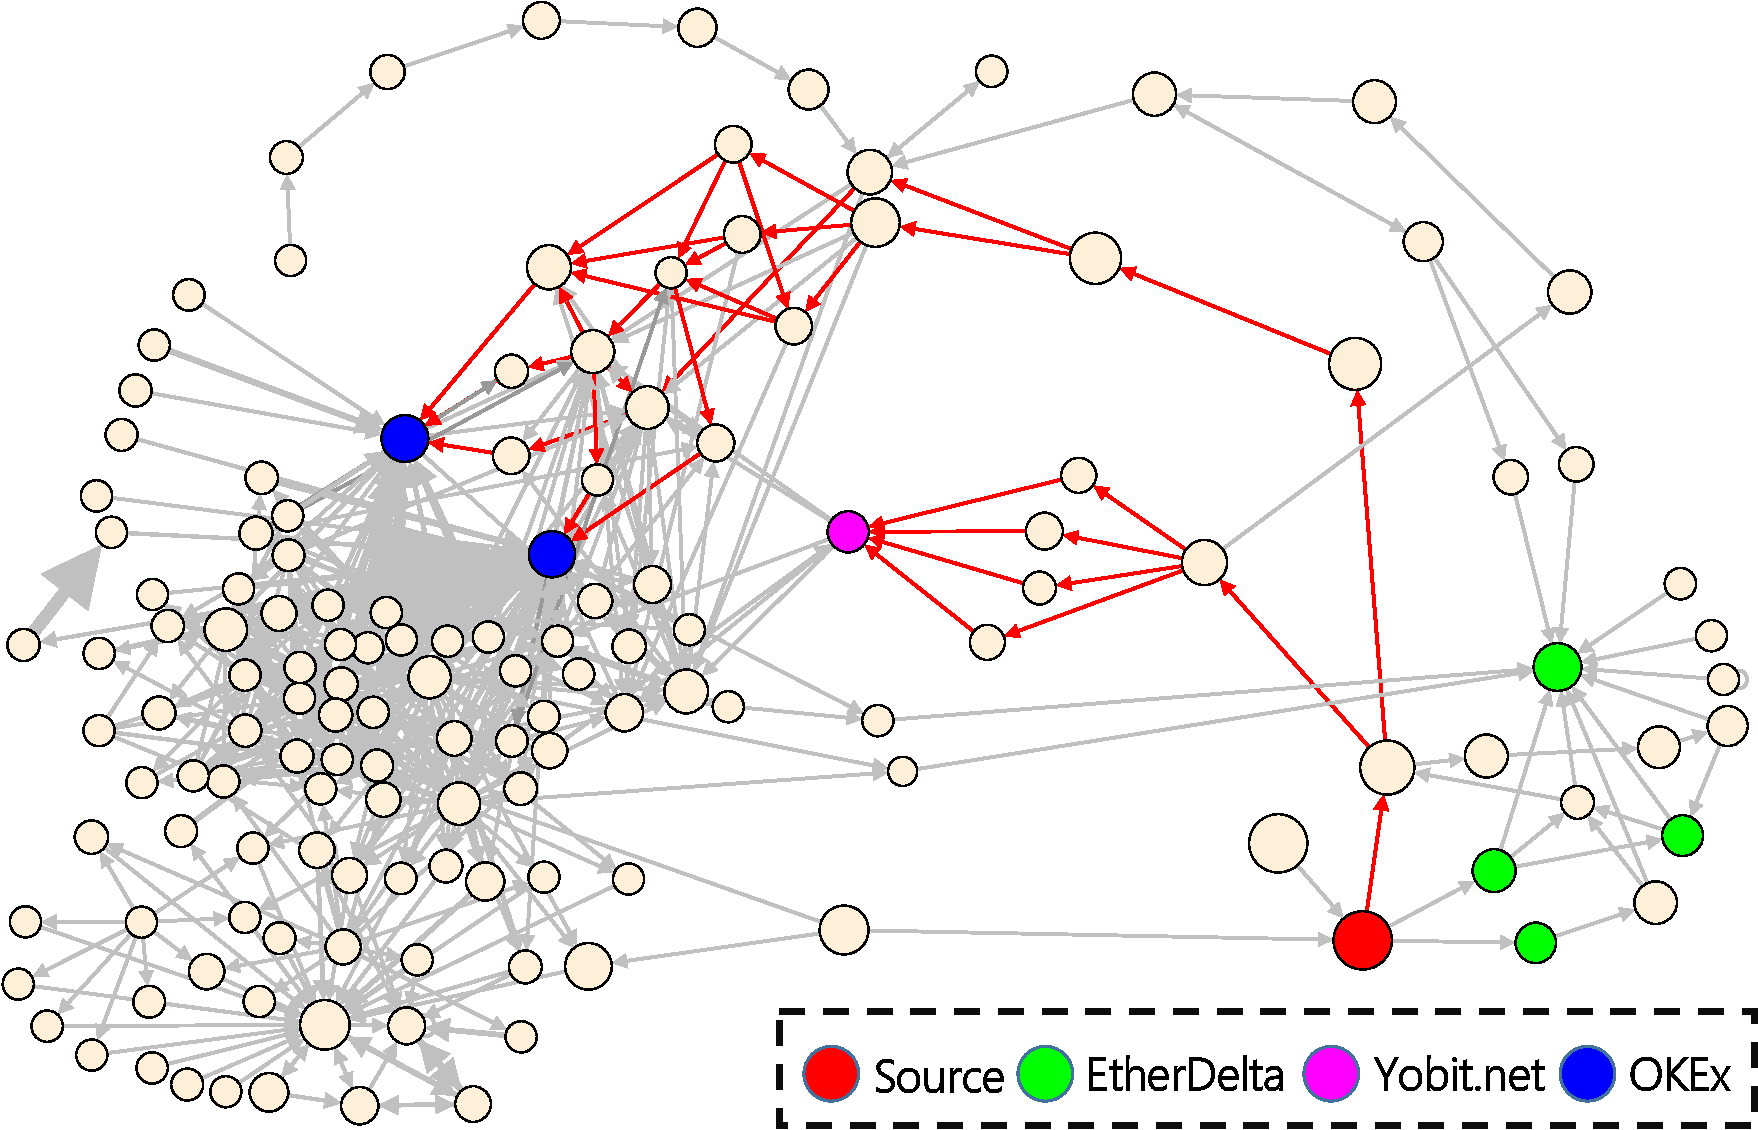
\includegraphics[width=0.8\linewidth]{figures/cryptopia.pdf}
    \caption{Tracing visualization for Cryptopia. Besides the EtherDelta exchange marked by experts, our method also finds the other target exchanges including Yobit.net and OKEx.}
    \label{fig:ttr_example_cryptopia}
\end{figure}
The Cryptopia exchange was attacked by hackers in May 2019.
According to the tracing result published by CoinHolmes\footnote{https://trace.coinholmes.com}, the source node with prefix 0xd4e79 \footnote{https://etherscan.io/address/0xd4e79226f1e5a7a28abb58f4704e53cd364e8d11} possessed 30.8K stolen ETH from Cryptopia and transferred about 10K ETH to 4 target nodes labeled as EtherDelta.

Figure \ref{fig:ttr_example_cryptopia} presents the transaction tracing result of our method, where the source node and the target nodes are marked with labels. 
Additionally, the node size is proportional to its rank score for each node, so the higher the rank is, the larger the node diameter is.
Based on the tracing result, we can find 4 target nodes labeled as EtherDelta (an exchange) in the 2-hop neighborhood of the source node easily, which is consistent with the results in CoinHolmes.

Moreover, another 4-hop neighbor of the source node labeled as Yobit.net\footnote{https://etherscan.io/address/0xf5bec430576ff1b82e44ddb5a1c93f6f9d0884f3} and two nodes labeled as OKEx can be found in the figure, which is not reported by CoinHolmes.
In fact, Yobit.net and OKEx are exchanges enabling the hacker to cash out the stolen ETH.
% In this way, Yobit.net and OKEx are reasonable to be target nodes.
According to the traced money flows in the figure, about 1420 stolen ETH is transferred into Yobit.net, and 18.47K stolen ETH is transferred into OKEx.
Therefore, more than 97\% of the stolen ETH of Cryptopia are traced by our method in this case. 

% Moreover, another 4-hop neighbor of the source node, labeled as Yobit.net with the address prefix 0xf5bec \footnote{https://etherscan.io/address/0xf5bec430576ff1b82e44ddb5a1c93f6f9d0884f3}, can also be found in the figure, which is not discovered by CoinHolmes.
% In fact, Yobit.net is an exchange enabling the hacker to cash out the stolen ETH, which is reasonable to be a target node.
% And from these fund flow paths, we can find the other 1420 stolen ETH.

% Besides, we can find two nodes labeled as OKEx in the figure, which is the deposit address of the OKEx exchange. 
% According to the traced ETH flows in the figure, it's reasonable that the hackers cashed out another part of the stolen ETH via OKEx, which is about 18.47K ETH.
% Therefore, more than 97\% of the stolen ETH of Cryptopia can be found with our method in this case.

\subsubsection{Kucoin}
\begin{figure}[t]
    \centering
    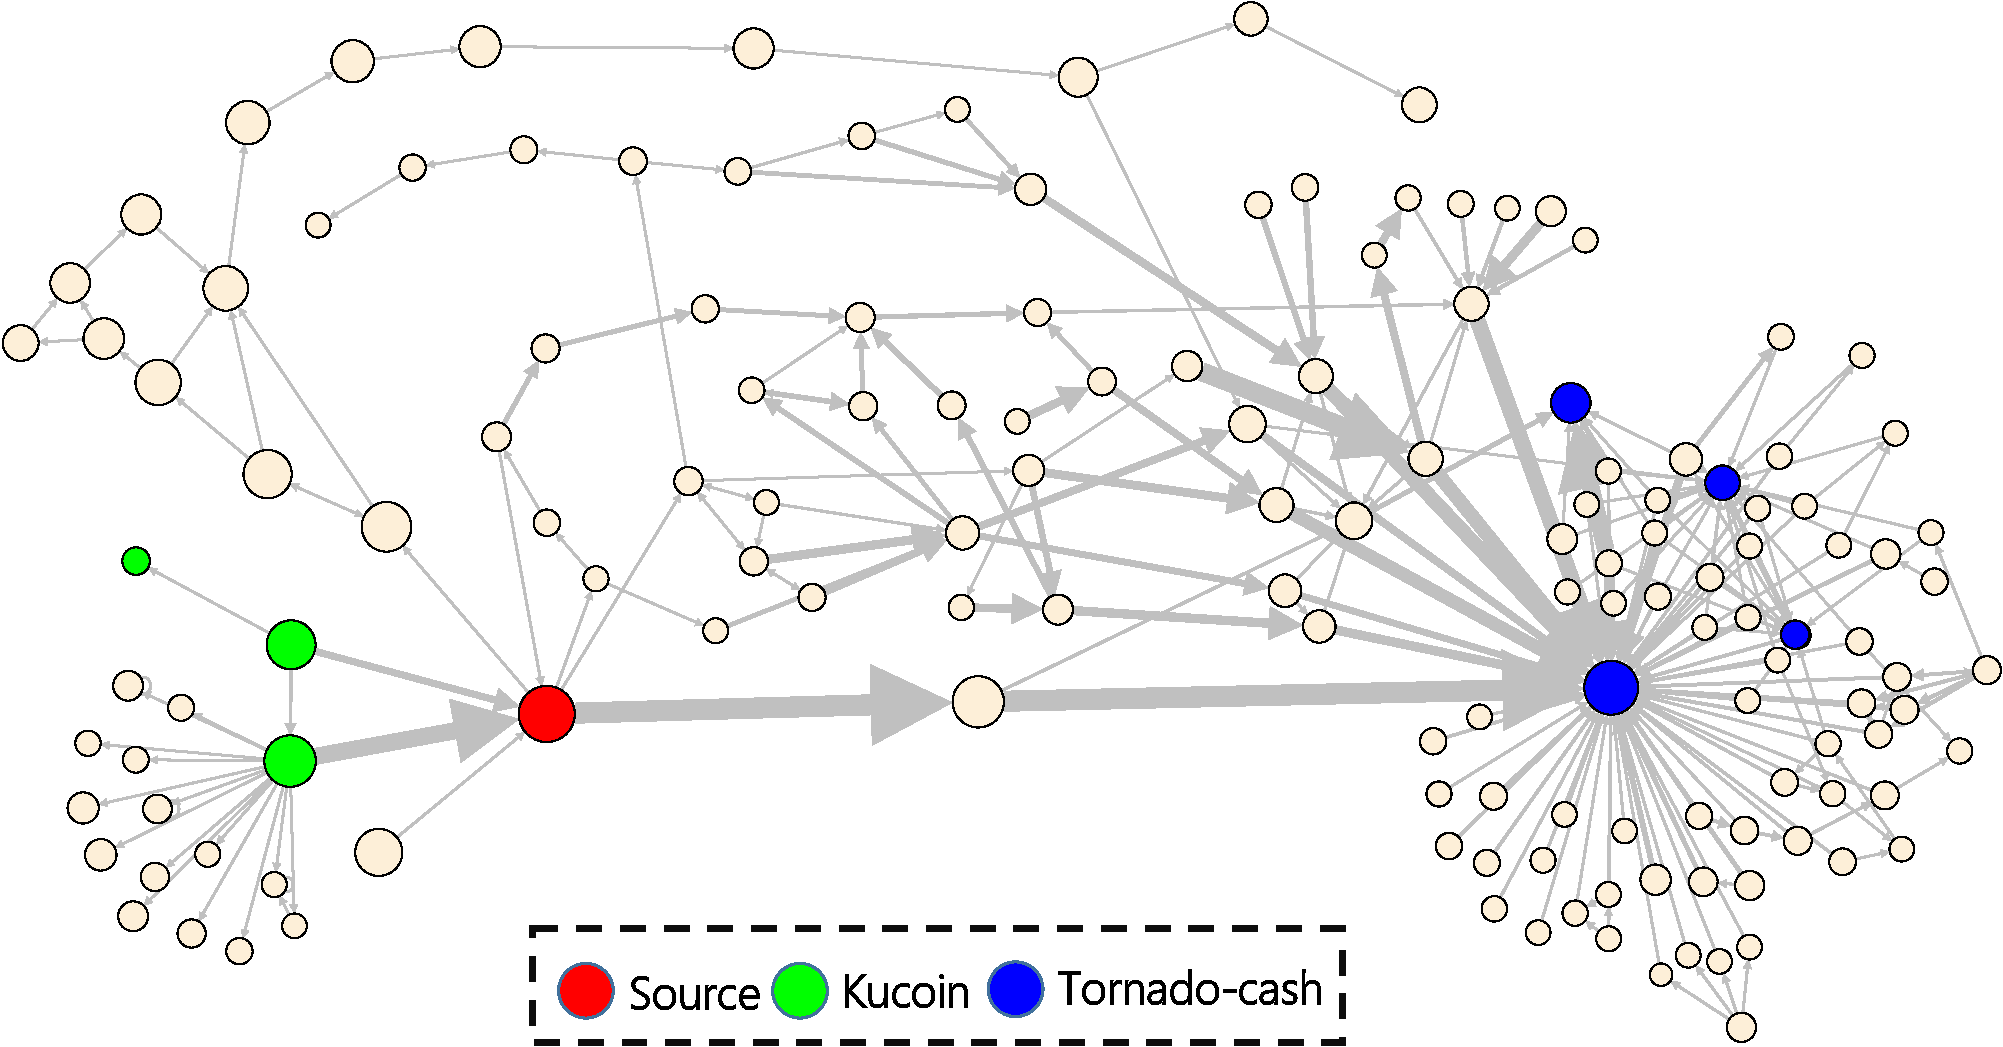
\includegraphics[width=0.95\linewidth]{figures/kucoin.pdf}
    \caption{Tracing visualization for Kucoin. A large number of ETH was transferred to Tornado Cash.}
    \label{fig:ttr_example_kucoin}
\end{figure}
The Kucoin exchange was attacked by hackers in September 2020, and there is still a large number of stolen funds that have not been traced until now.
As shown in Figure \ref{fig:ttr_example_kucoin}, the source node \footnote{https://etherscan.io/address/0xeb31973e0febf3e3d7058234a5ebbae1ab4b8c23} of the hackers obtained ETH from the nodes labeled as Kucoin, and then transferred most of the stolen ETH to a famous privacy-preserving protocol named Tornado Cash \cite{tornadocashdoc}.

Through the tracing result of our method, a total amount of 13.8K ETH was transferred to the 100 ETH pool of Tornado Cash, which is similar to the conclusion of experts in SlowMist\footnote{https://coinyuppie.com/uncovering-tornado-cashs-anonymity/}. As Tornado Cash is a decentralized mixing service, it is impossible for us to obtain valuable KYC information from this project to identify the hackers. 
In addition, since Tornado Cash is designed based on zero-knowledge proof, liquidity mining, and smart contract, it is difficult to trace the downstream fund flow when money is transferred into Tornado Cash. Therefore, some researchers have conducted analysis on Tornado Cash in recent years \cite{beres2020blockchain}.
\section{Conclusion}
\label{sec:conclusion}
In this paper, we studied the transaction tracing problem on account-based blockchain trading systems and proposed the first intelligent transaction tracing tool named TRacer. Compared with existing methods based on heuristics and taint analysis, which usually requires expert experience and manual intervention, TRacer show obvious superiority in terms of universality, effectiveness and time cost. In TRacer, we first formulated the transaction records in each account-based blockchain as a directed, weighted, temporal, and multi-relationship graph, which is able to represent the rich semantics of complex multi-token transaction relationships in the system. Then we proposed to use personalized PageRank-based graph searching technologies on this complex graph to trace the money flows. Specifically, we introduced novel approximate personalized PageRank strategies to realize effective and low-cost transaction tracing, which can also handle the complex DeFi transaction actions in account-based blockchains. The theoretical analysis and experimental results demonstrated the effectiveness of TRacer. 
% However, TRacer still cannot trace the fund flow using privacy enhancement technology, especially the mixing services such as Tornado Cash.
In the future, we will further delve into blockchain transaction tracing by integrating more transaction features like bytecodes and logs and design effective methods for blockchain systems with privacy-enhancing mechanisms.
% Moreover, our method can capture the subgraph of the source node, which will be used to carry out more effective node classification in future work.

%%
%% The acknowledgments section is defined using the "acks" environment
%% (and NOT an unnumbered section). This ensures the proper
%% identification of the section in the article metadata, and the
%% consistent spelling of the heading.
% \begin{acks}
% \end{acks}

%%
%% The next two lines define the bibliography style to be used, and
%% the bibliography file.
\bibliographystyle{ACM-Reference-Format}
\bibliography{bibfile}

%%
%% If your work has an appendix, this is the place to put it.
\appendix

% \section{Appendices}

\subsection{Proof of Theorem \ref{thm:run_time}}
\begin{proof}
This follows from Andersen et al. \cite{andersen2006local}, Lemma 2.
\end{proof}

\subsection{Proof of Theorem \ref{thm:push_cost}}
\begin{proof}
The residual of a node $u$ coming from its neighbors ensures that the number of non-zero elements in $R_s(u)$ are less than $|E(u)|$, where $E(u)$ contains edges related to $u$, so the cost of selfPush will not exceed $O(E(u))$.
In addition, forwardPush and backwardPush are both related to the timestamp of edges, so all edges among node $u$ and its neighbors can be sorted according to their timestamp firstly, whose cost is $O(|E(u)|log(|E(u)|))$, and then the summation terms are calculated in a timestamp order, whose cost is $O(|E(u)|)$.
Therefore, the cost of the local push procedure is:
\begin{equation}
    O( |E(u)|log(|E(u)|) + |E(u)| ) = O(|E(u)|log(|E(u)|)).
\end{equation}
\end{proof}

\subsection{Proof of Proposition \ref{pot:ttr_max_height}}
\begin{proof}
In order to maximize the estimate of $\bm{p}_s$ for the nodes having a high order of the source node, $\alpha$ needs to be as small as possible, and $\beta$ needs to be as close as possible to 0 or 1, which ensures that the residual can be pushed to a specific direction.
%  for reducing the dissipation caused by shunting
Considering $\beta=1$ here, the sum of residual pushed from the source node $s$ to the neighbors of order 1 to order $n$ are:
\begin{equation}
    \begin{cases}
        & r^{(1)}=(1-\alpha), \\
        & r^{(2)} \geq (1-\alpha)(r^{(1)}-k_1 \epsilon)=(1-\alpha)^2-(1-\alpha)k_1 \epsilon, \\
        & ...... \\
        & r^{(n)} \geq (1-\alpha)(r^{(n-1)}-k_{n-1} \epsilon) \\
        & \ \ \ \ \ \ \ \ =(1-\alpha)^n-\sum\limits_{i=1}^{n-1}(1-\alpha)^{n-i}k_{n-i} \epsilon, \\
    \end{cases}
\end{equation}
where $k_i$ represents the number of nodes with residual less than $\epsilon$ in the $i$-order neighbors of the source node.
Therefore, $r^{(n)}$ obtains the maximum value when:
\begin{equation}
    \sum\limits_{i=1}^{n-1}(1-\alpha)^{n-i}k_{n-i} \epsilon = 0,
\end{equation}
which means the residual of each $i$-order node greater or equal than $\epsilon$. 
This situation exists when the source node in a path graph, whose adjacency matrix satisfies $A(i,i+1)=1$ and other elements are $0$.
Consider the end condition of the local push procedure, the residual of $n$-order neighbors is:
\begin{equation}
    r^{(n)}=(1-\alpha)^n \leq \epsilon \Rightarrow n \leq \frac{log(\epsilon)}{log(1-\alpha)}.
\end{equation}
\end{proof}

\subsection{Proof of Proposition \ref{pot:ttr_local_comm}}
\begin{proof}
Consider the end condition of TTR-based Local Community Discovery Algorithm:
\begin{equation}
    \Phi(S)=\frac{\bm{p}_s(\partial(S))}{\bm{p}_s(S)} < \varphi,
\end{equation}
and the selfPush procedure at the first iteration of TTR Algorithm ensures:
\begin{equation}
    \bm{p}_s(s) \geq \alpha.
\end{equation}
Since $s \in S$, then $\bm{p}_s(S) \geq \alpha$, so:
\begin{equation}
    \bm{p}_s(\partial(S))<\varphi \alpha,
\end{equation}
which means that the path between $s$ and $v_n$ must be included in the local tracking network when $\bm{p}_s(v_n) \geq \varphi \alpha$. 
In this way, $\bm{p}_s(v_n)$ can obtain a minimum value with only one selfPush operation for $v_n$, and then $\bm{p}_s(v_n) \geq \varphi \alpha$ needs:
\begin{equation}
    % \alpha \sum_t r(v_n)(t) \geq \varphi\alpha \\
% \Rightarrow \sum_t r(v_n)(t) \geq \varphi.
    \alpha ||R_s(v_n)|| \geq \varphi \alpha \Rightarrow ||R_s(v_n)|| \geq \varphi
\label{equ:proof_ttr_local_comm_phi_target}
\end{equation}
Moreover, in order to ensure that at least one selfPush operation on $v_n$, the residual of $v_n$ must be greater than $\epsilon$, that is:
\begin{equation}
    \varphi \geq \epsilon.
\end{equation}
Consider that satisfying Equation \ref{equ:proof_ttr_local_comm_phi_target} in the worst case: 
1) The path between the source node and a target node is weakly connected, which makes the tracking tendency invalid.
2) The edges related to each node on the paths among the source node and the target node have the same weight, which makes the weight pollution invalid. 
3) Each path between the source node and a target node without increasing or decreasing timestamp, which makes time reasoning invalid.
4) There is only one path between the source node and a target node.
In this case, in order to satisfy the Equation \ref{equ:proof_ttr_local_comm_phi_target}, the residual sum of $m$-order neighbors ($m \leq n$) of the target node $v_n$ are:
\begin{equation}
    \begin{cases}
        & r^{(n)} \geq \varphi, \\
        & r^{(n-1)} \geq \frac{\varphi d_{n-1}}{min(\beta,1-\beta)(1-\alpha)}, \\
        & r^{(n-2)} \geq \frac{\varphi d_{n-1}d_{n-2}}{min^2(\beta,1-\beta)(1-\alpha)^2}, \\
        & ......\\
        & r^{(n-m)} \geq \frac{\varphi \prod\limits_{i=1}^{m}d_{n-i}}{min^m(\beta,1-\beta)(1-\alpha)^m},
    \end{cases}
\end{equation}
where $d_{n-i}$ denotes the degree of the $n-i$ order node in this path.
Consider the inequality as follow:
\begin{equation}
    \prod\limits_{i=1}^{m}d_{n-i} \leq (\frac{1}{m}\sum\limits_{i=1}^{m}d_{n-i})^m \rightarrow \bar{d}^m.
\end{equation}
If the $m$-order neighbor of the target node is the source node, then:
\begin{equation}
    1 \geq \frac{\varphi \bar{d}^n}{min^n(\beta,1-\beta)(1-\alpha)^n}
\Rightarrow \bar{d}\varphi^{\frac{1}{n}} \leq (1-\alpha) \cdot min(\beta,1-\beta)
\end{equation}
\end{proof}

\end{document}
\endinput
%%
%% End of file `sample-sigconf.tex'.


\section{Experiments}
\label{sec:experiments}
In this section, we conduct experiments to evaluate the effectiveness of TRacer on a large-scale real-world dataset. Besides, we conduct case studies with network visualization techniques.

\subsection{Experimental Setups}
% 主要包括参数设置、数据集描述、指标、对比算法

\subsubsection{Dataset}
We contribute a benchmark dataset including 20 transaction tracing cases in the recent 5 years across three account-based blockchains, i.e., Ethereum, Binance Smart Chain, and Polygon. 
These cases are initialized by various illegal activities containing hacker attacks, Rug-pull, and scams which have caused billions of dollars in losses. 
All these cases are reported by blockchain security companies and verified by experts coming from Certik \footnote{https://www.certik.com/}, Peckchield \footnote{https://peckshield.com/}, Chainalysis \footnote{https://www.chainalysis.com/} and so on.
Some statistics of this dataset are shown in Table \ref{tab:dataset}. 
Note that the transaction data in the dataset is obtained from the open APIs\footnote{https://blockscan.com}.
As we can see, the activities of these cases have acrossed millions of blocks, and we have to trace the money flows of the sources among more than 4 billion transactions.

\begin{table}[t]
  \caption{Statistics of the transaction record data related to the cases }
  \label{tab:dataset}
  \begin{tabular}{l|l|l}
    \hline
    \textbf{Field} & \textbf{Description} & \textbf{Number} \\
    \hline
    Source nodes & \tabincell{l}{The source node related to this\\case, such as the hacker account\\ and the scam contract.} & 20 \\ \hline
    Target nodes & \tabincell{l}{A set of target nodes related to\\this case, such as exchange\\wallets and mixing services.}  & 0.87K \\ \hline
    Blocks & \tabincell{l}{The blocks related to these cases.}  & 23.5M \\ \hline
    Transactions & \tabincell{l}{The transactions contained in the\\blocks related to these cases.} & 4.83B \\ \hline
  \end{tabular}
\end{table}
% Experiments are started from the source node in these cases in order to find the target nodes.

% \begin{table}[t]
%     \caption{Statistics of Cases}
%     \centering
%     \begin{threeparttable}
%         \begin{tabular}{cccccc}
%             \hline
%             Case & Source\tnote{1} & \#Target & \#Node & \#Edge & Block\tnote{2}\\
%             \hline
%             PlusToken & 0xf4a2e & 17 & 68 & 164 & 7993213\\
%             TokenStore & 0x068ac & 5 & 80 & 194 & 7802134\\
%             Cryptopia & 0xd4e79 & 4 & 9 & 24 & 9128188\\
%             Kucoin & 0xeb319 & - & - & - & 10933499\\
%             Upbit & 0xa0987 & - & - & - & 9007863\\
%             \hline
%         \end{tabular}
%         \begin{tablenotes}    
%             \footnotesize              
%             \item[1] Here provides the address prefix of the source node.
%             \item[2] Here provides the block number of the first transaction related to the cases.
%         \end{tablenotes}  
%     \end{threeparttable}
%     \label{tab:cases}
% \end{table}

% \begin{table*}[htb]
%     \caption{Experimental Results.}
%     \centering
%     \begin{threeparttable}
%         \begin{tabular}{cccccccccccccccc}
%             \hline
%              & \multicolumn{3}{c}{PlusToken} & \multicolumn{3}{c}{TokenStore} & \multicolumn{3}{c}{Cryptopia} & \multicolumn{3}{c}{Kucoin} & \multicolumn{3}{c}{Upbit} \\ \cmidrule(r){2-4} \cmidrule(r){5-7} \cmidrule(r){8-10} \cmidrule(r){11-13} \cmidrule(r){14-16}
%             Methods & $D_l$ & $K$ & $R$ & $D_l$ & $K$ & $R$ & $D_l$ & $K$ & $R$ & $D_l$ & $K$ & $P_l$ & $D_l$ & $K$ & $P_l$\\ \hline
%             BFS & 4.0$\times 10^{-9}$ & 3 & \textbf{0.93} &
%                 1.6$\times 10^{-7}$ & 3 & 0.4 &
%                 3.4$\times 10^{-7}$ & 3 & 1.0 &
%                 1.1$\times 10^{-8}$ & 3 & - &
%                 3.8$\times 10^{-9}$ & 3 & -\\
%             Poison & 6.3$\times 10^{-9}$ & 3 & 0 &
%                 1.6$\times 10^{-7}$ & 3 & 0.4 &
%                 2.3$\times 10^{-6}$ & 3 & 1.0 &
%                 2.3$\times 10^{-8}$ & 3 & - &
%                 6.4$\times 10^{-6}$ & 3 & -\\
%             Haircut & 7.6$\times 10^{-9}$ & \textbf{6} & \textbf{0.93} &
%                 8.1$\times 10^{-8}$ & \textbf{6} & \textbf{1.0} &
%                 7.0$\times 10^{-8}$ & 7 & \textbf{1.0}\tnote{*} &
%                 2.0$\times 10^{-5}$ & 4 & - &
%                 4.0$\times 10^{-7}$ & 5 & -\\
%             APPR & 0 & 0 & 0 &
%                 8.1$\times 10^{-4}$ & 5 & 0.4 &
%                 3.1$\times 10^{-4}$ & 7 & \textbf{1.0}\tnote{*} &
%                 6.0$\times 10^{-4}$ & 4 & 0.25 &
%                 2.4$\times 10^{-4}$ & 4 & 0.26\\
%             \hline
%             TTR-base & 4.9$\times 10^{-5}$ & 5 & \textbf{0.93} & 
%                 \textbf{2.0}\bm{$\times$}\textbf{10}$^{-3}$ & 5 & 0.4 & 
%                 4.0$\times 10^{-4}$ & 6 & \textbf{1.0}\tnote{*} & 
%                 \textbf{6.2}\bm{$\times$}\textbf{10}$^{-4}$ & 4 & 0.26 & 
%                 2.8$\times 10^{-4}$ & 6 & 0.44\\
%             TTR-weight & 2.2$\times 10^{-5}$ & \textbf{6} & \textbf{0.93} & 
%                 2.8$\times 10^{-4}$ & \textbf{6} & \textbf{1.0} & 
%                 6.9$\times 10^{-4}$ & 7 & \textbf{1.0}\tnote{*} & 
%                 2.7$\times 10^{-4}$ & 5 & 0.39 & 
%                 4.0$\times 10^{-4}$ & \textbf{8} & \textbf{0.75}\\
%             TTR-time & \textbf{1.2}\bm{$\times$}\textbf{10}$^{-4}$ & 5 & \textbf{0.93} &
%                 1.6$\times 10^{-4}$ & \textbf{6} & \textbf{1.0} &
%                 \textbf{9.6}\bm$\times$\textbf{10}$^{-4}$ & \textbf{10} & \textbf{1.0}\tnote{*} &
%                 2.2$\times 10^{-4}$ & \textbf{7} & \textbf{0.52} & 
%                 \textbf{4.3}\bm$\times$\textbf{10}$^{-4}$ & \textbf{8} & 0.65\\
%              \hline
%         \end{tabular}
%         \begin{tablenotes}    
%             \footnotesize              
%             \item[*] These methods can find some extra suspicious target nodes, referring to Section \ref{sec:case_study_Cryptopia}.
%         \end{tablenotes}
%     \end{threeparttable}
%     \label{tab:experimentations}
% \end{table*}

\subsubsection{Compared Methods}
We compare our method with several baseline blockchain transaction tracing methods. For a fair comparison, we use the general framework of TRacer to reproduce the following comparison methods, including:
\begin{itemize}
    \item \textbf{BFS} \cite{zhao2015graph}: Breadth-First Search, which is the first and the most commonly used transaction tracing method.
    \item \textbf{Poison} \cite{moser2014towards}: A kind of taint analysis technology in blockchain transaction tracing. Each output of a transaction with a dirty input is considered to be tainted in this method.
    \item \textbf{Haircut} \cite{moser2014towards}: A kind of taint analysis technology in blockchain transaction tracing. Each output of a transaction with a dirty input is considered to be tainted partially according to the amount value in this method. 
    \item \textbf{APPR} \cite{andersen2006local}: The approximate personalized PageRank algorithms, which can calculate the relevance of nodes in a network to a given source node with an extremely low cost.
    % \item \textbf{TRacer}: The method we proposed, where the graph construction recognizes the transaction patterns, the TTR and greedy selection are used for graph expansion, and the local community detection is applied in Extract.
    % using a novel local push procedure, and we abbreviate the TTR algorithm with tracing tendency, weight pollution, and temporal reasoning strategies as TTR-base, TTR-weight, and TTR-time respectively.
\end{itemize}

The details of implementing the above transaction tracing technologies can be found in our GitHub page \footnote{https://github.com/wuzhy1ng/BlockchainSpider}.

\subsubsection{Experimental Settings} 
% {\color{blue}Based on the experiences, it is enough for BFS and Poison to trace the 2-order neighbors of the source node, since the increase of order leads to the exponential growth of the size of subgraph in graph expansion for these two methods, bringing great difficulty to transaction auditing.}
%%  !!!! 这段话大有问题
Since the increase of depth can lead to the exponential growth of the size of output graph in BFS and Poison, bringing great difficulty to transaction auditing. During our experiments, we set the upper limit of the tracing depth in these two methods is 2. In addition, we use the Haircut method to trace the ``dirty money'' from the source node until the amount proportion of ``dirty money" of all nodes is less than 0.1\% of that from the source node.
Moreover, we set $\alpha=0.15$, $\epsilon=10^{-3}$ for APPR and TTR, and $\varphi=10^{-3}$, $\beta=0.7$ for TTR to ensure that our method is able to find the paths among the source node and the target nodes with 42-hop at most, according to Proposition \ref{pot:max_depth}.

\subsubsection{Metrics}
we report the average of the following metrics in all cases to measure the effectiveness of transaction tracing:
% We use the following metrics to measure the effectiveness of transaction tracing:
\begin{itemize}
    \item \textbf{Recall}: The recall evaluates how many target nodes can be traced by a method, which is defined as: $Recall = \frac{|V_t|}{|\bar{V_t}|}$, where $|V_t|$ is the number of traced target nodes and $|\bar{V_t}|$ is the number of all target nodes in a case.
    
    \item \textbf{Number of nodes}: This metric measures the number of nodes in the output graph of a case. A smaller output graph with recall ensured is easier for expert auditing.
    % Ensuring the recall, the fewer node number, the more conducive to expert verification.
    
    \item \textbf{Tracing depth}: This metric measures how deep can a transaction tracing method traverse the transaction graph from a source node, indicating that up to $K$-hop neighbors of the source node are detected.
\end{itemize}

\subsection{Experimental Results}
% 参数敏感性实验
\subsubsection{Scalability vs. Performance}
\begin{figure}[t]
    \centering
    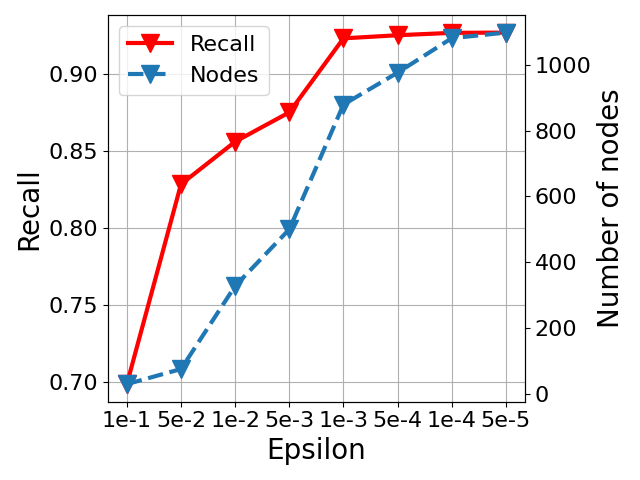
\includegraphics[width=0.65\linewidth,height=3.7cm]{figures/epsilon_metrics.png}
    \vskip -0.1in
    \caption{The relationship among Epsilon, Recall, and Node number. Note that the recall has reached 70\% with $\epsilon = 10^{-1}$ merely, and the increment of recall becomes slow when $\epsilon$ is less than $10^{-3}$.}
    \label{fig:epsilon_metrics}
\end{figure}
The approximation parameter $\epsilon$ is an important hyper-parameters in modulating the scalability.
To examine the effect of $\epsilon$ on the performance, we repeat experiments with different values of $\epsilon$ and report the recall as well as the number of traced nodes. 
As Figure \ref{fig:epsilon_metrics} shows, the recall has reached 70\% when $\epsilon = 10^{-1}$.
When $\epsilon$ is less than $10^{-3}$, the increment of recall becomes slow, and the number of nodes rapidly increases. 
Therefore, setting $\epsilon = 10^{-3}$ can guarantee a higher recall and fewer nodes with a relatively low cost in experiments, and we set $\epsilon = 10^{-3}$ for TRacer.
% , which is the reason why we set $\epsilon = 10^{-3}$ for TRacer.


% 对比实验
\subsubsection{Comparative experiment}
\begin{table}[t]
  \caption{
  Performance comparison between baselines and TRacer
%   Comparative experiment results. Besides the number of tracing nodes being more than APPR slightly, the recall and tracing depth are better than other methods significantly.
  }
  \label{tab:compared_methods}
  \begin{tabular}{cccc}
    \toprule
    Methods & Recall (\%) & Number of nodes (K) & Tracing depth\\
    \midrule
    BFS & 77.02 & 52.50 & 2.00\\
    Poison & 70.06 & 41.45 & 2.00\\
    Haircut & 58.85 & 10.35 & 4.15\\
    APPR & 71.92 & \textbf{0.66} & 3.60\\
    \textbf{TRacer} & \textbf{92.31} & 0.87 & \textbf{5.05}\\
  \bottomrule
\end{tabular}
\end{table}
Table \ref{tab:compared_methods} shows the performance of different methods, from which we can obtain the following observations.
\textbf{\textit{Firstly}}, the output graphs of BFS and Poison contain an extremely large number of nodes, which brings great difficulty to transaction auditing even through detecting more than 70\% target nodes.
\textbf{\textit{Secondly}}, the output graph of Haircut has fewer nodes than BFS and Poison with a greater tracing depth, but the recall is too low to achieve effective tracing.
\textbf{\textit{Thirdly}}, fewest nodes are obtained by APPR, ensuring the detection results can be easier audited by experts. 
\textbf{Fourthly}, TRacer obtains better performance than APPR. On the basis of the advantages of APPR, the recall and tracing depth of TRacer are significantly better than other methods.

% 消融实验
\subsubsection{Ablation experiment}
\begin{table}[t]
  \caption{Ablation experiment.}
  \label{tab:ablation_experiment}
  \setlength{\tabcolsep}{0.1mm}{
  \begin{tabular}{p{2.5cm}<{\centering}p{1.4cm}<{\centering}p{2.2cm}<{\centering}|p{0.6cm}<{\centering}p{1.8cm}<{\centering}}
    \toprule
    Graph construction with DeFi patterns & Graph expansion & Local community detection & Recall (\%) & Number of nodes (K)\\
    % pattern recognition & expansion & detection & (\%) & of nodes (K)\\
    \midrule
    $\surd$ & $\surd$ & $\surd$ & 92.3 & 0.87\\
     & $\surd$ & $\surd$ & 80.3 & 0.55\\
    $\surd$ & $\surd$ &  & 95.9 & 57.5\\
  \bottomrule
\end{tabular}}
\end{table}
TRacer is consist of three modules including graph construction, graph expansion, and local community detection. 
In order to discuss the function of different modules, we conduct an ablation study and report the performance of TRacer in Table \ref{tab:ablation_experiment} after removing the DeFi pattern recognition in graph construction and the local community detection.
% remove the graph construction module recognizing the edge patterns or local community detection module extracting the important local community, and report the performance as shown in Table \ref{tab:ablation_experiment}.
When the DeFi pattern recognition is removed in the graph construction module, the recall decreases significantly, which shows that the understanding of DeFi patterns in TRacer can help trace the money flows effectively.
Moreover, if the local community detection module is removed, the number of nodes increases significantly with the weakly improvement of recall, which shows that the local community detection module can find the nodes strongly associated with the source node at the cost of a small recall loss.

% Top N recall
\subsubsection{Top\textit{N} Recall}
\begin{figure}[t]
    \centering
    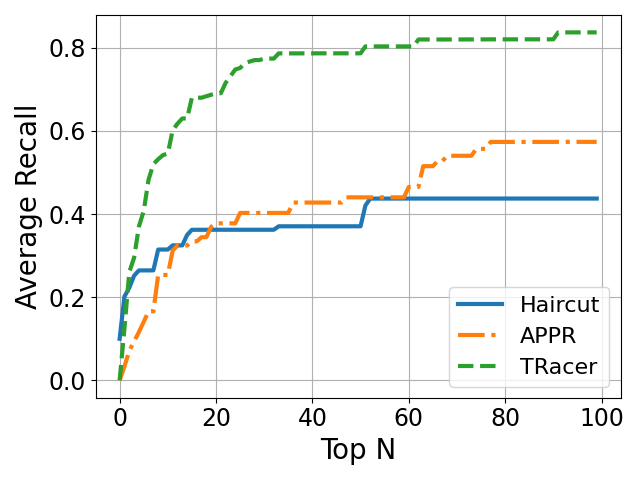
\includegraphics[width=0.6\linewidth]{figures/topn_recall_v2.png}
    \caption{Top $n$ most relevant nodes and the recall. 
    % TRacer tends to give higher importance to the target nodes.
    }
    \label{fig:topn_recall}
\end{figure}

Since the rank of a node represents the relevance relationship between this node and the source node, we can audit the nodes according to the descending order of rank. To compare the rank-based methods including Haircut, APPR, and TRacer, we take out the top $n$ most relevant nodes to the source and calculate the recall for different $n$.
The result is displayed in Figure \ref{fig:topn_recall}, where the curve of TRacer shows a better performance than other methods.
In addition, TRacer achieves a 25\% recall gain over APPR when $n>50$.

\subsection{Case Study}
\label{sec:case_study}
% 该部分对案例中的TTR局部交易网络进行分析
% In this part, we visualize the fund flow on cases with verified labels by Gephi 0.9.2 \cite{bastian2009gephi}.
In this part, we visualize the traced money flow of two cases with Gephi 0.9.2 \cite{bastian2009gephi}, in order to evaluate the feasibility of TRacer.
% In this section, we give the analysis of cases with the local tracing network captured by our method through gephi.

\subsubsection{Cryptopia}\label{sec:case_study_Cryptopia}
\begin{figure}[t]
    \centering
    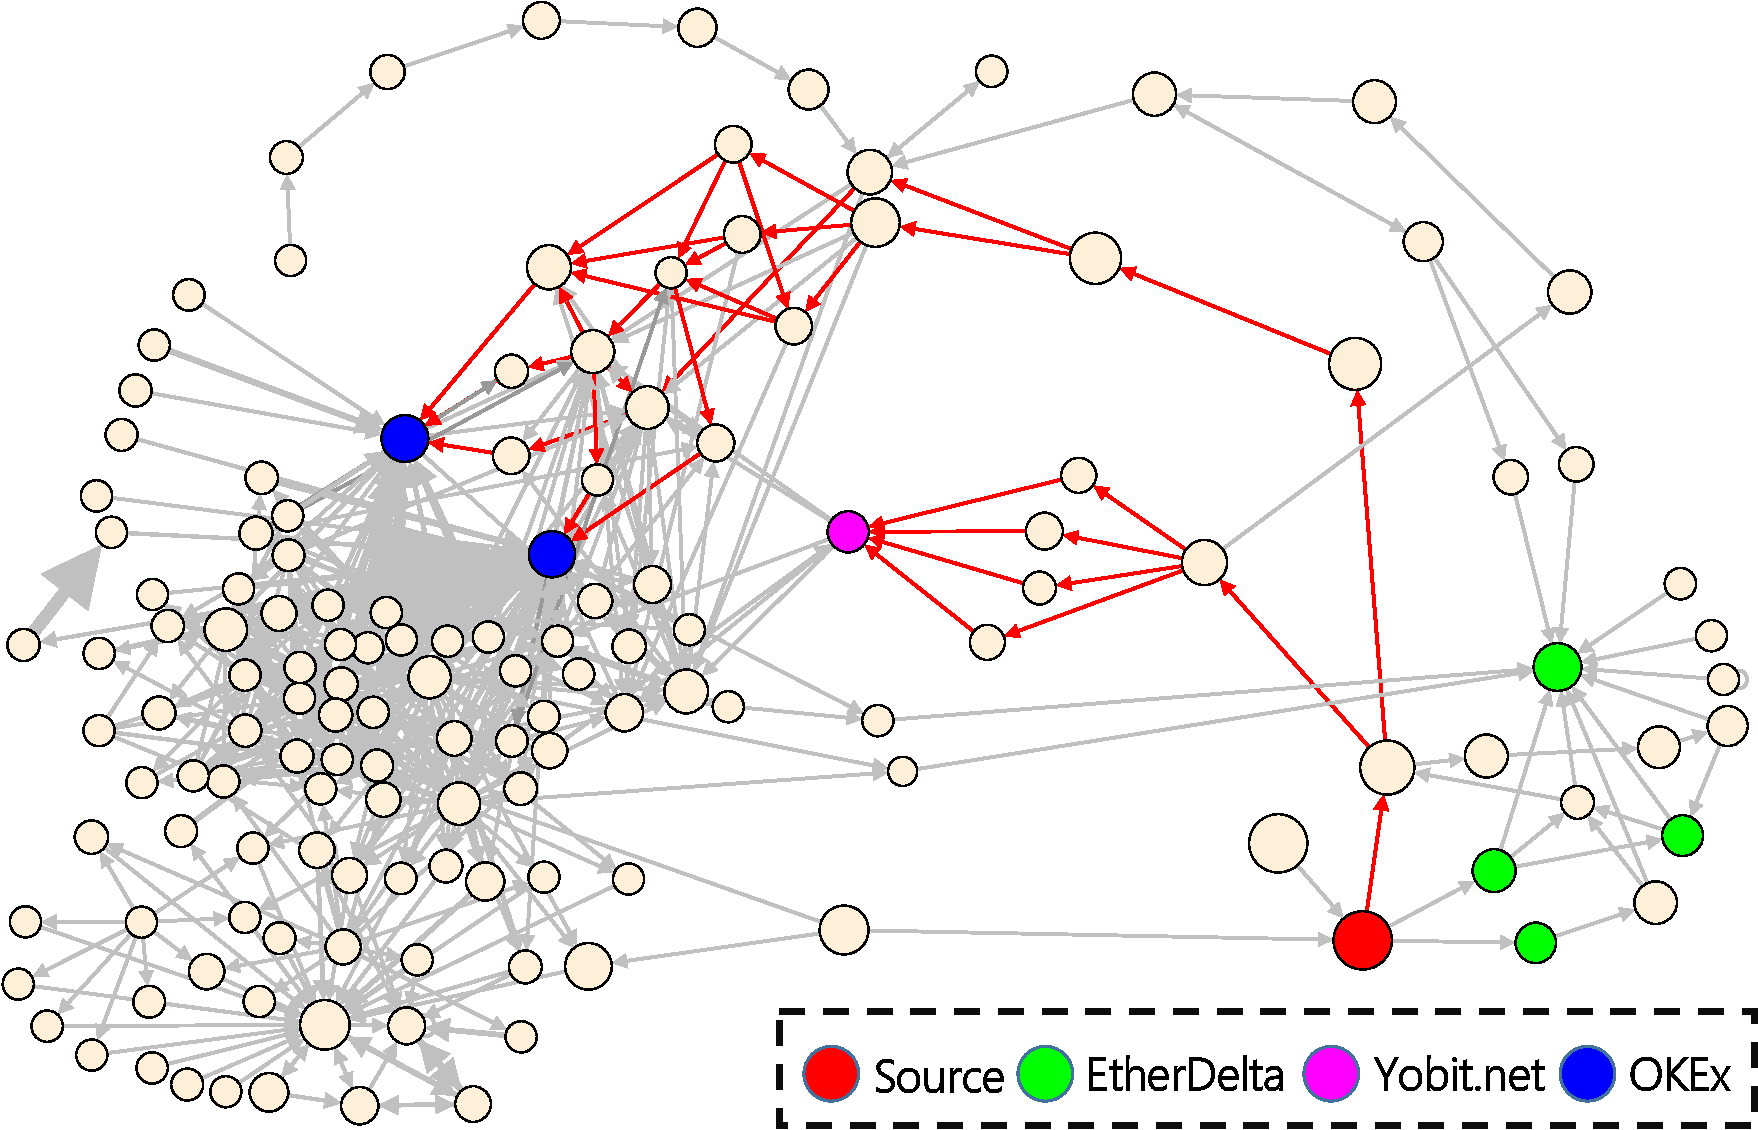
\includegraphics[width=0.8\linewidth]{figures/cryptopia.pdf}
    \caption{Tracing visualization for Cryptopia. Besides the EtherDelta exchange marked by experts, our method also finds the other target exchanges including Yobit.net and OKEx.}
    \label{fig:ttr_example_cryptopia}
\end{figure}
The Cryptopia exchange was attacked by hackers in May 2019.
According to the tracing result published by CoinHolmes\footnote{https://trace.coinholmes.com}, the source node with prefix 0xd4e79 \footnote{https://etherscan.io/address/0xd4e79226f1e5a7a28abb58f4704e53cd364e8d11} possessed 30.8K stolen ETH from Cryptopia and transferred about 10K ETH to 4 target nodes labeled as EtherDelta.

Figure \ref{fig:ttr_example_cryptopia} presents the transaction tracing result of our method, where the source node and the target nodes are marked with labels. 
Additionally, the node size is proportional to its rank score for each node, so the higher the rank is, the larger the node diameter is.
Based on the tracing result, we can find 4 target nodes labeled as EtherDelta (an exchange) in the 2-hop neighborhood of the source node easily, which is consistent with the results in CoinHolmes.

Moreover, another 4-hop neighbor of the source node labeled as Yobit.net\footnote{https://etherscan.io/address/0xf5bec430576ff1b82e44ddb5a1c93f6f9d0884f3} and two nodes labeled as OKEx can be found in the figure, which is not reported by CoinHolmes.
In fact, Yobit.net and OKEx are exchanges enabling the hacker to cash out the stolen ETH.
% In this way, Yobit.net and OKEx are reasonable to be target nodes.
According to the traced money flows in the figure, about 1420 stolen ETH is transferred into Yobit.net, and 18.47K stolen ETH is transferred into OKEx.
Therefore, more than 97\% of the stolen ETH of Cryptopia are traced by our method in this case. 

% Moreover, another 4-hop neighbor of the source node, labeled as Yobit.net with the address prefix 0xf5bec \footnote{https://etherscan.io/address/0xf5bec430576ff1b82e44ddb5a1c93f6f9d0884f3}, can also be found in the figure, which is not discovered by CoinHolmes.
% In fact, Yobit.net is an exchange enabling the hacker to cash out the stolen ETH, which is reasonable to be a target node.
% And from these fund flow paths, we can find the other 1420 stolen ETH.

% Besides, we can find two nodes labeled as OKEx in the figure, which is the deposit address of the OKEx exchange. 
% According to the traced ETH flows in the figure, it's reasonable that the hackers cashed out another part of the stolen ETH via OKEx, which is about 18.47K ETH.
% Therefore, more than 97\% of the stolen ETH of Cryptopia can be found with our method in this case.

\subsubsection{Kucoin}
\begin{figure}[t]
    \centering
    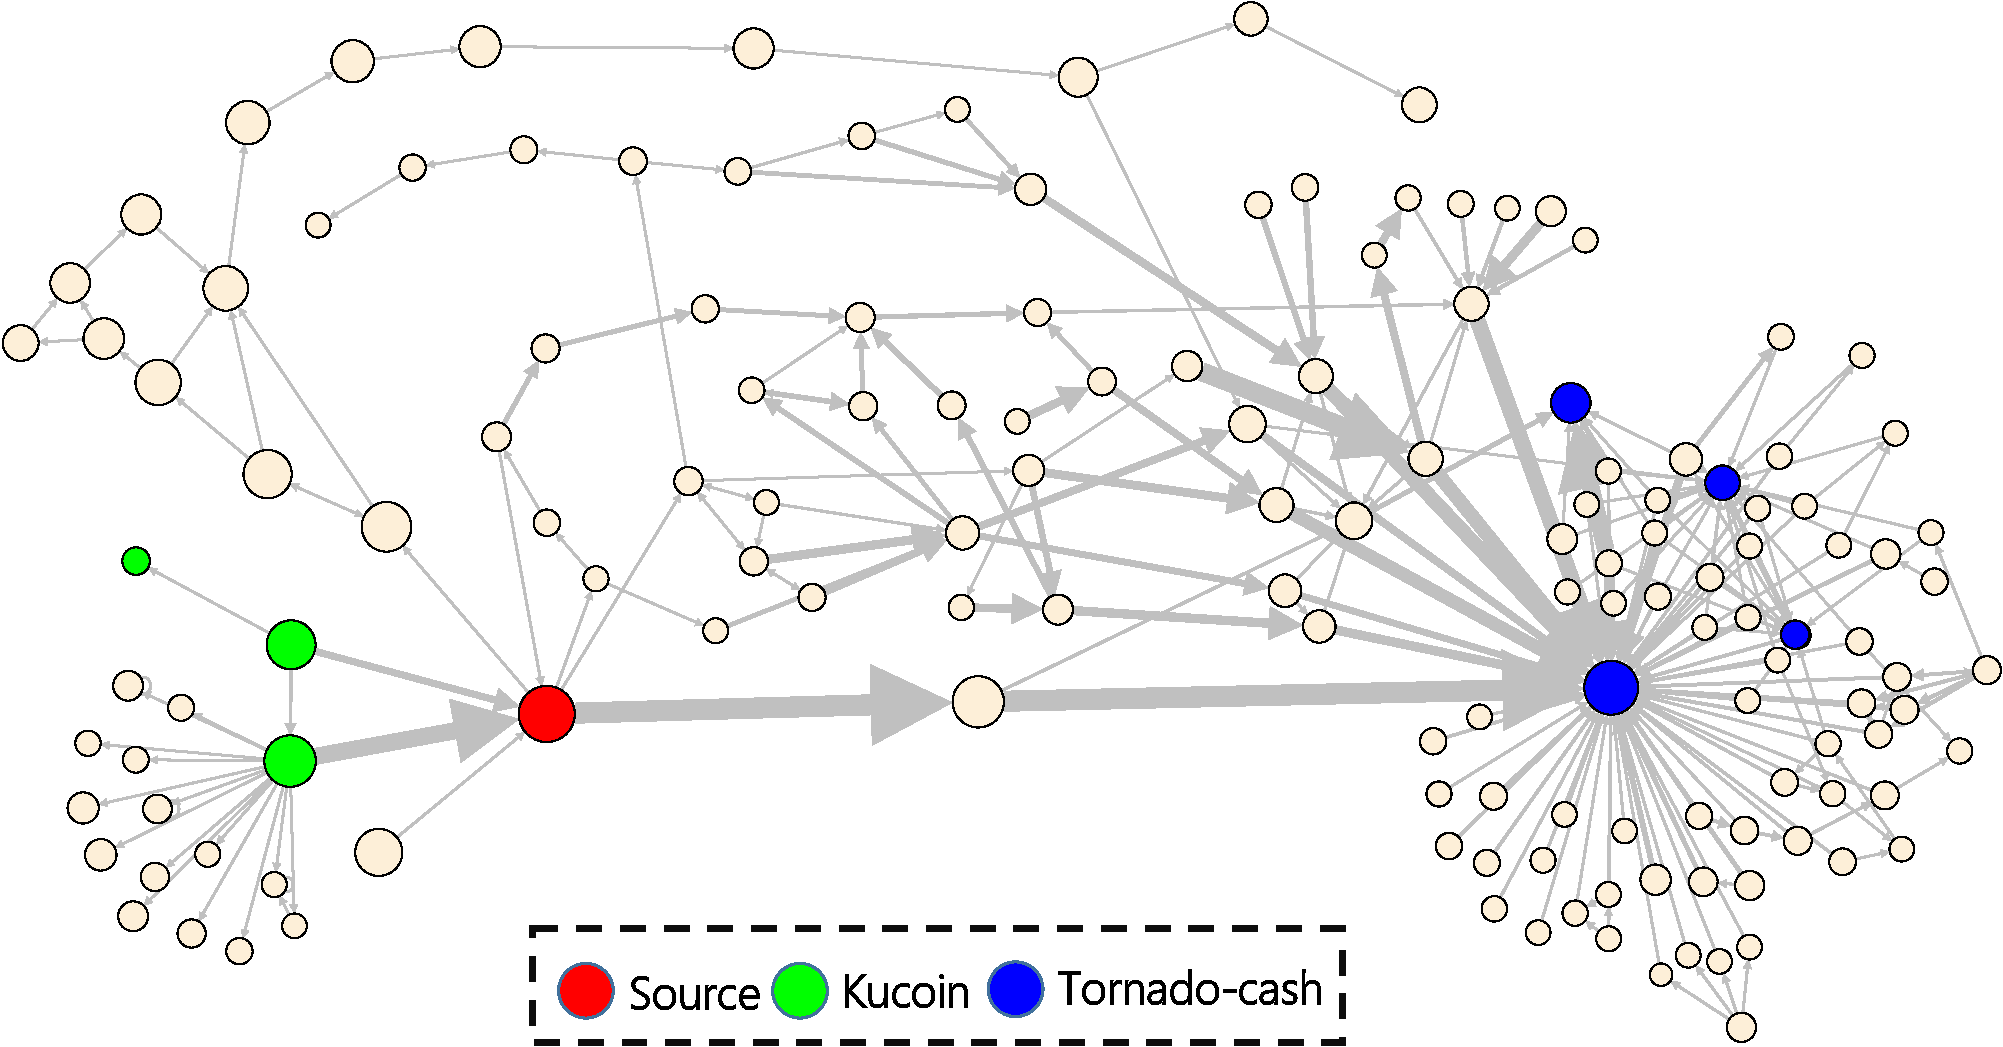
\includegraphics[width=0.95\linewidth]{figures/kucoin.pdf}
    \caption{Tracing visualization for Kucoin. A large number of ETH was transferred to Tornado Cash.}
    \label{fig:ttr_example_kucoin}
\end{figure}
The Kucoin exchange was attacked by hackers in September 2020, and there is still a large number of stolen funds that have not been traced until now.
As shown in Figure \ref{fig:ttr_example_kucoin}, the source node \footnote{https://etherscan.io/address/0xeb31973e0febf3e3d7058234a5ebbae1ab4b8c23} of the hackers obtained ETH from the nodes labeled as Kucoin, and then transferred most of the stolen ETH to a famous privacy-preserving protocol named Tornado Cash \cite{tornadocashdoc}.

Through the tracing result of our method, a total amount of 13.8K ETH was transferred to the 100 ETH pool of Tornado Cash, which is similar to the conclusion of experts in SlowMist\footnote{https://coinyuppie.com/uncovering-tornado-cashs-anonymity/}. As Tornado Cash is a decentralized mixing service, it is impossible for us to obtain valuable KYC information from this project to identify the hackers. 
In addition, since Tornado Cash is designed based on zero-knowledge proof, liquidity mining, and smart contract, it is difficult to trace the downstream fund flow when money is transferred into Tornado Cash. Therefore, some researchers have conducted analysis on Tornado Cash in recent years \cite{beres2020blockchain}.
\section{Proposed Approach}
\label{sec:proposed_approach}
% This section introduces the Push-Pop model and designs the TTR algorithm in Push-Pop model for blockchain transaction tracking.
This section introduces the architecture, implementation, and theoretical analysis of TRacer.

\subsection{Architecture Overview}
TRacer consists of three main modules including graph construction, graph expansion, and local community detection. Each module is described as follows:
\begin{itemize}
\item \textbf{Graph construction}: This module models the money transfer relationships between accounts as directed, weighted, temporal, and multi-relationship graphs.
% in which the nodes and the edges represent the accounts and the transactions in the blockchain, respectively.
\item \textbf{Graph expansion}: Since the blockchain data contains billions of transactions which is too large for common graph algorithms, this module aims to find a relevant subgraph from a risky source. The module contains four operations: \textit{\textbf{Expand}} collects all edges related to a given node, \textit{\textbf{Push}} merges the collected edges to the subgraph, \textit{\textbf{Rank}} computes the relevance of nodes in the subgraph to the source, and \textit{\textbf{Pop}} selects a node for expanding.
The graph expansion process terminates when the end condition is met.
\item \textbf{Local community detection}: This module \textit{\textbf{Extract}}s a local community of the source node from the expended subgraph, in which nodes have higher relevance to the source than nodes out of the community.
\end{itemize}

\subsection{Graph construction}
Since there are multiple types of tokens in account-based blockchain trading systems, we formulate the money transfer relationships among accounts into a directed, weighted, temporal, and multi-relationship graph $G=(V, E)$, where $V$ is the node set representing accounts, $E$ is the edge set representing the token transfer relationships.
% with $\varphi_E: E\rightarrow\{{\rm token \ types}\}$ for edge-type mapping
% , and $X$ denotes the set of attributes attached to edges including transaction hash (unique to the corresponding external transaction), amount, timestamp, and token symbol. 
An edge $e=(u,v,w,t,b,h)$ denotes that account $u$ transfer $w$ units token $b$ to account $v$ at timestamp $t$ with a transaction hash $h$. We define mapping functions $f_{src}$, $f_{tgt}$, $f_{amt}$, $f_{ts}$, and $f_{sym}$ to map each edge to its source, target, amount, timestamp, and token type respectively. There are multiple types of edges indicating the transfer relationships of different tokens.

In addition, many blockchain services such as decentralized exchanges act as the intermediary for token swap. 
To reveal the token flows after users interact with these services, we categorize the money transfer relationships into two patterns, namely \textbf{Xfer} and \textbf{Swap}.
As shown in Figure \ref{fig:Xfer}, accounts send or receive tokens through the Xfer pattern, and the related DeFi actions \cite{wu2021defiranger} in this pattern include: 1) \textbf{\textit{transfer}}: An account sends an amount of token to another account, 2) \textbf{\textit{minting}}: A token contract mints an amount of token to an account, and 3) \textbf{\textit{burning}}: An account burns an amount of token.
While accounts exchange tokens for other kinds of tokens through the Swap pattern as shown in Figure \ref{fig:Swap}, including three related DeFi actions: 1) \textbf{\textit{add liquidity}}: An account deposits an amount of token to a DeFi app, and receives a certain amount of Liquidity Provider (LP) token back, 2) \textbf{\textit{remove liquidity}}: An account sends an amount of LP token to a DeFi app for destroying and gets a certain amount of other tokens back, and 3) \textbf{\textit{trade}}: An account sells an amount of token A in a DeFi app for a certain amount of token B. We identify the transaction relationships involving both the sending of tokens and the receiving of another kind of tokens with the same hash as the relationships in the Swap pattern, and otherwise as the relationships in the Xfer pattern. 
% In this way, we define the pattern mapping for the edges in the transaction graph:
% \begin{equation}
%     P: E \rightarrow \{Xfer, Swap\}.
% \end{equation}

% In addition, considering the token transfer, there are two types of patterns for a transaction in TRacer, namely \textbf{Xfer} and \textbf{Swap}.
% A transaction is recognized as Swap if the transactions with the same transaction hash ensure an account sending and receiving tokens at the same time, otherwise Xfer.
% These two patterns are summarized from the transaction actions defined by token contracts and DeFi DApps. 
% Several main actions \cite{wu2021defiranger} are listed below:
% \begin{itemize}
%     \item \textbf{Transfer}: An account sends an amount of token to another account.
%     \item \textbf{Minting}: A token contract sends an amount of minted token to an account. 
%     \item \textbf{Burning}: An account sends an amount of token to a token contract for destroying.
%     \item \textbf{Add Liquidity}: An account deposits an amount of token to the DeFi app, which also sends its an amount of Liquidity Provider (LP) token to the account.
%     \item \textbf{Remove Liquidity}: An account sends an amount of LP token to a DeFi app for destroying, and the account gets a number of other tokens back.
%     \item \textbf{Trade}: An account sells an amount of token A in a DeFi app for a certain amount of token B.
% \end{itemize}

\begin{figure}[t]
    \centering
    \subfigure[The Xfer pattern]{
    
\includegraphics[width=0.3\linewidth]{figures/Xfer.png}
    \label{fig:Xfer}
    }
    \subfigure[The Swap pattern] {
    
\includegraphics[width=0.35\linewidth]{figures/Swap.png}
    \label{fig:Swap}
    }
    \caption{(a) Xfer: Sending or receiving tokens.
    % Transaction actions in this pattern include transfer, minting, and destroying. 
    (b) Swap: Exchanging tokens for other kinds of tokens. 
    % Transaction actions in this pattern include add liquidity, remove liquidity, and trade.
    }
\end{figure}

\subsection{Graph Expansion}
The graph expansion module aims to obtain a relevant subgraph expanded from a given seed via iterating four operations shown in Figure \ref{fig:TRacer}. In what follows, we introduce the design of these four operations.
\subsubsection{\textit{Push} and \textit{Rank}: Transaction Tracing Rank}
The \textit{Push} operation merges the expanded edges to the subgraph in each iteration. While \textit{Rank} calculates the relevance of nodes in the subgraph to the source.
% While Rank is the core operation of graph extension in TRace, which determines the rules for calculating the relevance of nodes to the source node in the subgraph.

We introduce APPR to calculate the node relevance. 
More specifically, the Rank operation executes the local push procedure for the incremental update of node relevance.
% Especially, according to some characteristics of the transaction graph in account-based blockchain, we design a novel local push procedure. 
% The relevance computed using this novel local push procedure is named \textbf{Transaction Tracing Rank} (TTR).
Based on the characteristics of blockchain transaction graph in account-based blockchains, we propose a novel local push algorithm named \textbf{\underline{T}ransaction \underline{T}racing \underline{R}ank (TTR)} to compute the node relevance in blockchain transaction graph. We develop four local push strategies in TTR, namely \textbf{tracing tendency, weighted pollution, temporal reasoning, and token redirection}. We use $r_s(u,t,b)$ to denote the residual of node $u$ brought from token $b \in B$ at timestamp $t \in \Gamma$, where $\Gamma$ is the timestamp set and $B$ is the token symbol set in the subgraph.
% In the local push procedure of TTR, the edge attributes of time and token symbol need to be considered, thus we use $r_s(u,t,b)$ to denote the residual attached with a timestamp $t \in \Gamma$ and a token symbol $b \in B$ in the node $u$, where $\Gamma$ is a set of timestamps, and $B$ is a set of token symbols.
% % the residual is stored by a dictionary structure with the definition below:
% % \begin{equation}
% %     r_s: V \times \Gamma \times B \rightarrow \mathbb{R},
% %     \label{req:residual_mapping}
% % \end{equation}
% % where $V$ denotes a set of nodes, $\Gamma$ denotes a set of timestamps, and $B$ denotes a set of token symbols.
In this way, the local push procedure in TTR is described as Algorithm \ref{alg:ttr_local_push}. During initialization, a part of the residual of node $u$ is transformed into the relevance (line 1). Moreover, other parts of the residual are pushed to the neighbors according to the four strategies.
% 伪代码备份
% \begin{algorithm}[t]
%     \caption{TTR local push}
%     \label{alg:ttr_local_push}
%     \begin{algorithmic}[1]
%         \REQUIRE Node $u$, edges $E(u)$ related to $u$, rank $\bm{p}_s$, residual $r_s$, timestamp set $\Gamma$, and token symbol set $B$.
%         \ENSURE The updated $\bm{p}_s$ and $r_s$.
%         %% 自环
%         \STATE $\bm{p}_s(u) = \bm{p}_s(u) + \alpha \sum\limits_{b \in B}\sum\limits_{t \in \Gamma}r_s(u,t,b)$
%         \STATE $r'_s(u,t,b)=r_s(u,t,b), r_s(u,t,b)=0$ for $\forall t\in \Gamma, \forall b\in B$.
%         \FOR{$(t,b)$ in $\Gamma \times B$}
%             \STATE $res = r'_s(u,t,b)$
%             %% 出边
%             \STATE $E_{out}(u)=$ the edges of $u$ output token $b$ after timestamp $t$.
%             \STATE $W_{out}=$ the sum of edge weight in $E_{out}(u)$.
%             \FOR{$e$ in $E_{out}(u)$}
%                 % \STATE $E'_{out}(u)=$ the out-edges of $u$ swapped from $e$ recursively.
%                 \STATE $E'_{out}(u)=\rho(\{e\}, E(u))$.
%                 \STATE $r_s(v_{e'},t_{e'},b_{e'})+=\frac{(1-\alpha) \beta w_e}{W_{out}|E'_{out}(u)|} \times res$ for $\forall e' \in E'_{out}(u)$
%             \ENDFOR
%             %% 入边
%             \STATE $E_{in}(u)=$ the edges of $u$ input token $b$ before timestamp $t$.
%             \STATE $W_{in}=$ the sum of edge weight in $E_{in}(u)$.
%             \FOR{$e$ in $E_{in}(u)$}
%                 % \STATE $E'_{in}(u)=$ the in-edges of $u$ swapped from $e$ recursively.
%                 \STATE $E'_{in}(u)=\rho(\{e\}, E(u))$.
%                 \STATE $r_s(v_{e'},t_{e'},b_{e'})+=\frac{(1-\alpha) (1-\beta) w_e}{W_{in}|E'_{in}(u)|} \times res$ for $\forall e' \in E'_{in}(u)$
%             \ENDFOR
%             \STATE $r_s(u,t,b)=(1-\alpha)\beta r'_s(u,t,b)$ if $|E_{out}(u)|==0$.
%             \STATE $r_s(u,t,b)=(1-\alpha)(1-\beta) r'_s(u,t,b)$ if $|E_{in}(u)|==0$.
%         \ENDFOR
%         \RETURN $\bm{p}_s, r_s$
%     \end{algorithmic}
% \end{algorithm}


\begin{algorithm}[t]
    \caption{TTR local push}
    \label{alg:ttr_local_push}
    \begin{algorithmic}[1]
        \REQUIRE Node $u$, edges $E(u)$ related to $u$, edge mapping functions $f_{src}$, $f_{tgt}$, $f_{amt}$, $f_{ts}$, $f_{sym}$, rank $\bm{p}_s$, residual $r_s$,
        timestamps $\Gamma$, token symbols $B$, 
        teleport constant $\alpha$, and tracing tendency $\beta$.
        \ENSURE The updated $\bm{p}_s$ and $r_s$.
        %% 自环
        % \STATE $\Gamma=\{f_{ts}(e) | e\in E(u)\}$
        % \STATE $B=\{f_{sym}(e) | e\in E(u)\}$
        \STATE $\bm{p}_s(u) = \bm{p}_s(u) + \alpha \sum\limits_{b \in B}\sum\limits_{t \in \Gamma}r_s(u,t,b)$
        \STATE $r'_s(u,t,b)=r_s(u,t,b), r_s(u,t,b)=0$, $\forall t\in \Gamma, \forall b\in B$.
        \FOR{$(t,b) \in \Gamma \times B$}
            % \STATE $res = r'_s(u,t,b)$
            %% 出边
            \STATE $E_{out}=\{e\in E(u)|f_{ts}(e)>t\wedge f_{src}(e)=u\wedge f_{sym}(e)=b\}$
            \STATE $E_{in}=\{e\in E(u)|f_{ts}(e)<t\wedge f_{tgt}(e)=u\wedge f_{sym}(e)=b\}$
            \FOR{$E' \in \{ E_{out}, E_{in} \}$}
                % \STATE $W=\sum\limits_{e \in E'}f_{amt}(e)$.
                \STATE $\gamma = \beta \ if \  E'==E_{out} \ else \ (1-\beta)$
                \FOR{$e \in E'$}
                    \STATE $E'_{\rho}=\rho(\{e\}, E(u))$ // obtained by Equation \ref{equation:token_redirect}
                    \FOR{$e' \in E'_{\rho}$}
                        \STATE $\Delta = \frac{(1-\alpha)\gamma f_{amt}(e)}{|E'_{\rho}|\sum\limits_{e ''\in E'}f_{amt}(e'')} r'_s(u,t,b)$
                        \STATE $v=f_{src}(e') \ if \ E'==E_{in} \ else \ f_{tgt}(e')$
                        \STATE $r_s(v,f_{ts}(e'),f_{sym}(e'))+=\Delta$
                    \ENDFOR
                    % \STATE $r_s(f_{amt}(e'),f_{ts}(e'),f_{sym}(e'))+=\frac{(1-\alpha)\gamma f_{amt}(e)}{|E'_{\rho}|\sum\limits_{e \in E'}f_{amt}(e)} r'_s(u,t,b)$ for $e'\in E'_{\rho}$
                \ENDFOR
                \STATE $r_s(u,t,b)=(1-\alpha)\gamma r'_s(u,t,b)$ if $|E'|==0$.
            \ENDFOR
            % \STATE $r_s(u,t,b)=(1-\alpha)\beta r'_s(u,t,b)$ if $|E_{out}(u)|==0$.
            % \STATE $r_s(u,t,b)=(1-\alpha)(1-\beta) r'_s(u,t,b)$ if $|E_{in}(u)|==0$.
        \ENDFOR
        \RETURN $\bm{p}_s, r_s$
    \end{algorithmic}
\end{algorithm}
% In this way, the TTR local push procedure in a node $u$ can be described by the equations below:
% \begin{equation}
%     \begin{cases}
%         & \Delta \bm{p}_s(u) = \alpha \sum\limits_{b \in B} \sum\limits_{t \in \Gamma} r_s(u,t,b) \\ 
%         & \Delta r_s(v_{out},t,b) = (1-\alpha)\beta \rho 
%         \begin{pmatrix}
%         b, \theta 
%             \begin{pmatrix}
%             v_{out}, r_s, \tau(t,E(u))
%             \end{pmatrix}
%         \end{pmatrix}
%          \\ 
%         & \Delta r_s(v_{in},t,b) = (1-\alpha)(1-\beta) \rho
%         \begin{pmatrix}
%         b, \theta 
%             \begin{pmatrix}
%             v_{in}, r_s, \tau(t,E(u))
%             \end{pmatrix}
%         \end{pmatrix}
%     \end{cases},
% \end{equation}
% in which $t\in \Gamma$, $b \in B$, $v_{out} \in N_{out}(u)$ and $v_{in} \in N_{in}(u)$ denote out-degree neighbor and in-degree neighbor of $u$ respectively, $\beta$ denotes the tracing tendency coefficient controlling the attention for different neighbors, $\theta$ denotes a weight pollution function focusing on distributing the residual by edge weight, $\tau$ denotes the temporal reasoning function aiming to select edges with specific timestamps, $\rho$ denotes the token redirection function for processing the transaction patterns, and $E(u)$ denotes the edges related to the node $u$.

\textbf{Tracing tendency}.
Since a money transfer relationship between accounts is directed, the attention to in-degree neighbors and out-degree neighbors during the local push procedure can be different.
% For example, tracing for the target of the fund flows oriented from a particular source needs to pay more attention to its out-degree neighbors, while tracing for the source of money needs to pay more attention to the in-degree neighbors.
In most cases, tracing for the destinations of money flows oriented from a particular source needs to pay more attention to the out-degree neighbors. Therefore, we define an attention coefficient $0 \leq \beta \leq 1$. During the residual propagation, the out-degree neighbors in a transaction relationship can get a higher residual when $\beta > 0.5$, and the in-degree neighbors can receive a higher residual when $\beta < 0.5$. As Figure \ref{fig:TTR_strategies}(a) shows, the in-degree neighbors and the out-degree neighbors obtain a different weight in this strategy. Line 6-17 in Algorithm \ref{alg:ttr_local_push} describe the residual propagation procedure of different directions with the attention coefficient assigned at line 7. 
%Therefore, considering the transaction graph $G$ is directed and giving a tracing tendency coefficient $0 \leq \beta \leq 1$, the out-degree neighbors in a transaction relationship get a higher residual when $\beta > 0.5$ for tracing the target of the fund flow, and the in-degree neighbors in a transaction relationship get a higher residual when $\beta < 0.5$ for tracing the source of the fund flow.
% As Figure \ref{fig:tracing_tendency} shows, the out-degree neighbors of a node $u$ get a higher residual than the in-degree neighbors, when $\beta > 0.5$.
% In this way, the residual is split for pushing to out-degree neighbors and in-degree neighbors with different coefficients being $\beta$ and $1-\beta$ (line 7) in Algorithm \ref{alg:ttr_local_push}.

\textbf{Weighted pollution}. 
% Traditional APPR pushes the residual of a node to the neighbors by considering an equal weight during a local push procedure. 
% However, in a transaction relationship, the transaction strength is usually weighted by the transaction amount. 
% Note that the edge strength is usually weighted by the transaction amount.
In blockchain transaction graph, the strength of money transfer relationships is weighted by the transaction amount. For each node, a neighbor trading a larger amount of money with this node is considered to be more relevant to the node. 
% Therefore, by considering the transaction graph $G$ is weighted with the transaction amount information as the weight, 
Therefore, in this strategy we take the weight of the money transfer relationships into account. Figure \ref{fig:TTR_strategies}(b) shows an example of this strategy that neighbors of $u$ associated by edges with greater weight can obtain more residual during the propagation.
In this way, the residual of a node is distributed to each neighbor associated by edge $e \in E'$ according to the ratio of edge weight $f_{amt}(e) / \sum_{e'' \in E'}f_{amt}(e'')$ as shown in Algorithm \ref{alg:ttr_local_push} line 11, where $E'$ is the set of edges.

\textbf{Temporal reasoning}.
Blockchain transactions are recorded in blocks chronologically. Each block contains a specific timestamp. 
% Since the fund flow transferring process is dynamic, the transaction time information can be taken into consideration in the local push procedure.
With the timestamp information, tracing for the targets of money flows usually follows the paths with increasing timestamps, while tracing back to the source of money flows follows the paths with decreasing timestamps.
Therefore, in this strategy we take the temporal information into consideration. For example in Figure \ref{fig:TTR_strategies}(c), the residual from the input transaction at $t2$ is pushed out through the outgoing edges after $t2$ and the incoming edge before $t2$. Algorithm \ref{alg:ttr_local_push} line 4-5 show the edge set for residual propagation that satisfies this strategy.
% The timestamp is used to restrict the edges for pushing (line 4, 5) in Algorithm \ref{alg:ttr_local_push}.
Moreover, the residual is pushed to the node itself if the edge set is empty in Algorithm \ref{alg:ttr_local_push} line 16, indicating that the funds have not been transferred from the node.

\begin{figure}[t]
    \centering
    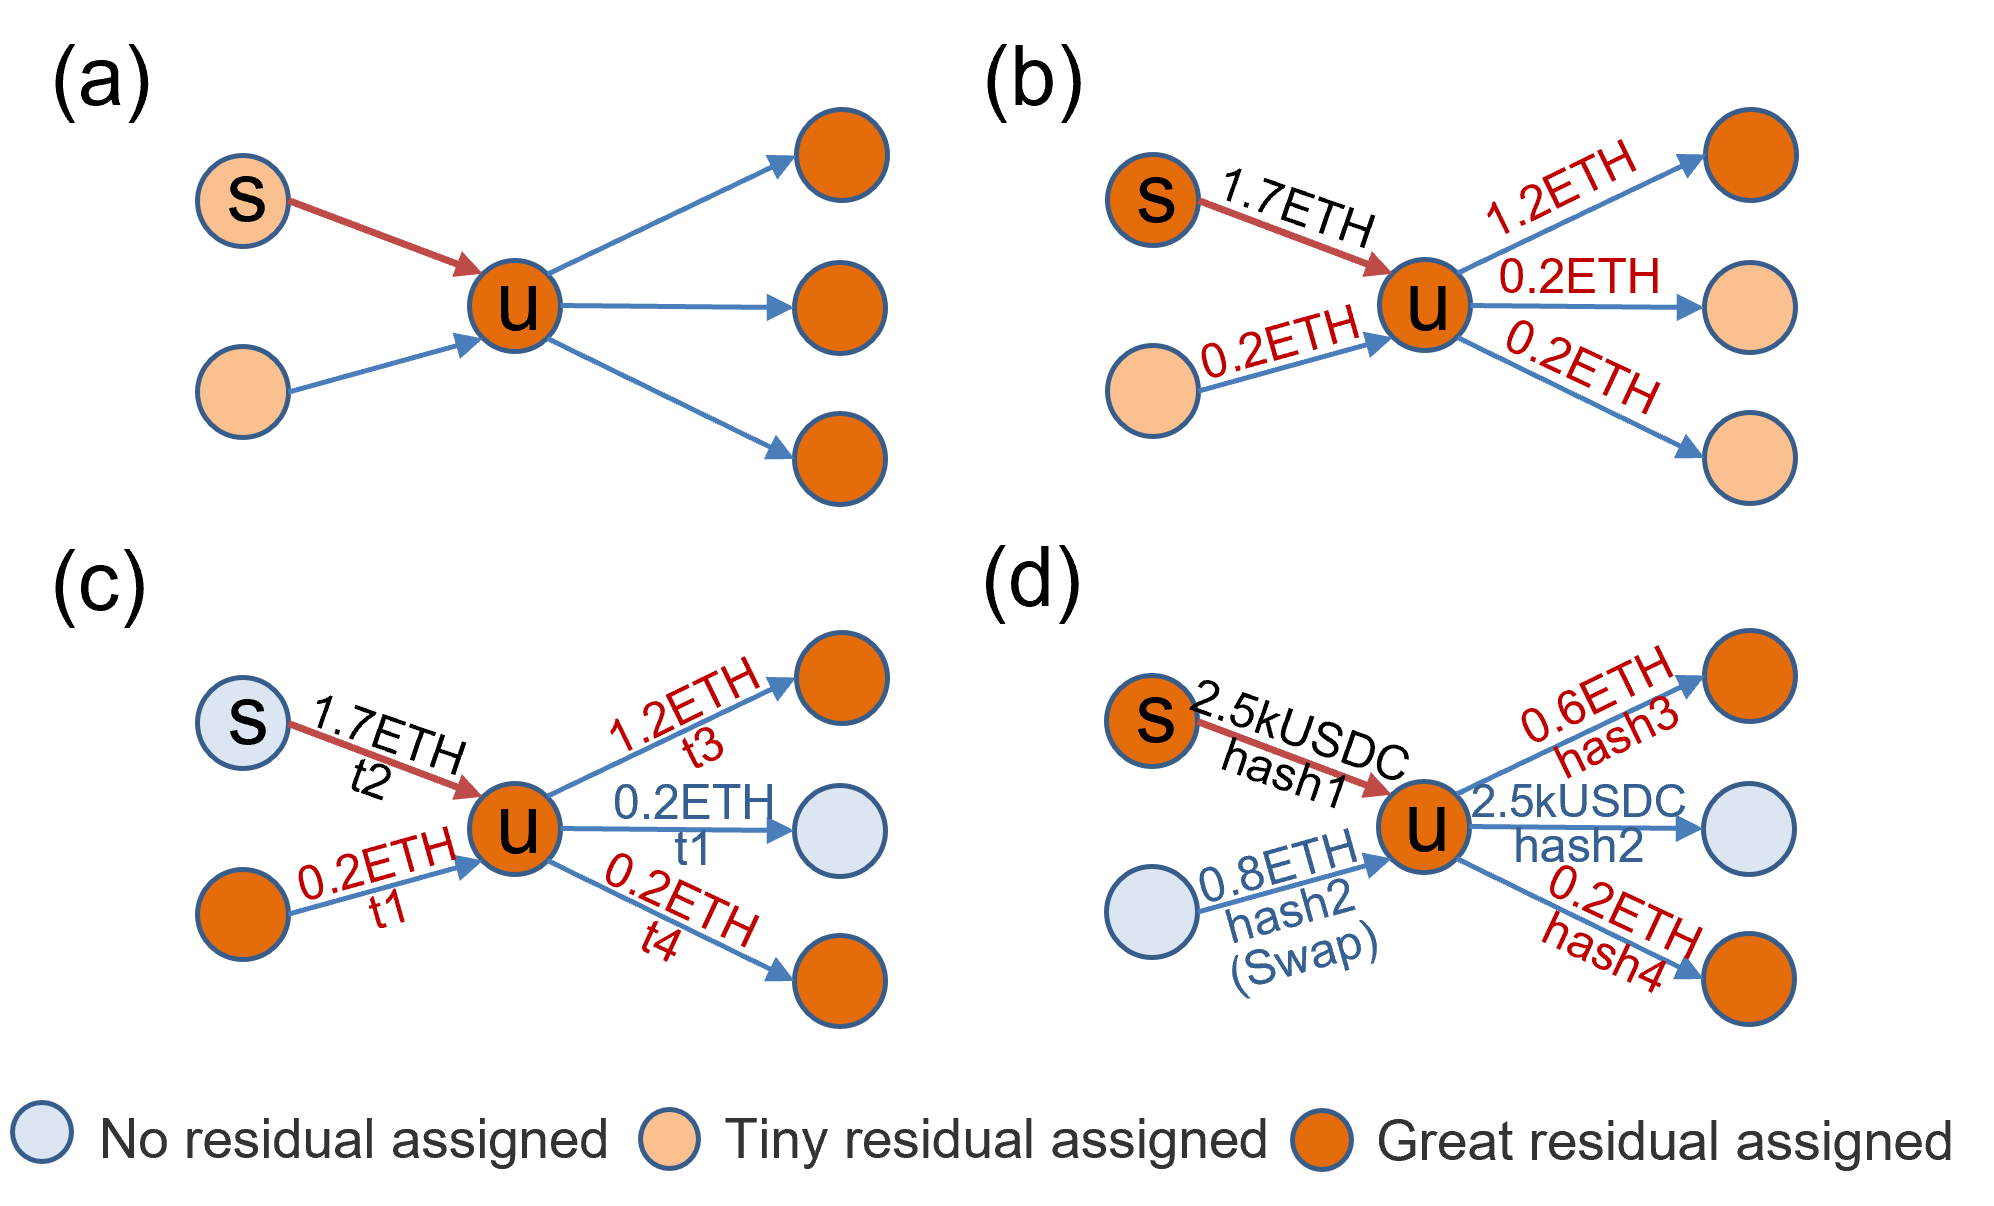
\includegraphics[width=0.9\linewidth]{figures/TTRstrategies.png}
    \caption{(a) Tracing tendency. 
    Different attention is assigned to the out-degree neighbors and in-degree neighbors.
    (b) Weighted pollution. The higher the edge weight, the closer the relationship. 
    (c) Temporal reasoning. Tracing money flow in chronological order, and $t1<t2<t3<t4$ in this example. 
    (d) Token redirection. Uncovering the token flows even though there exist complex DeFi actions in the Swap pattern.}
    \label{fig:TTR_strategies}
\end{figure}

% \begin{figure}[t]
%     \centering
%     \subfigure[Tracing tendency]{
%     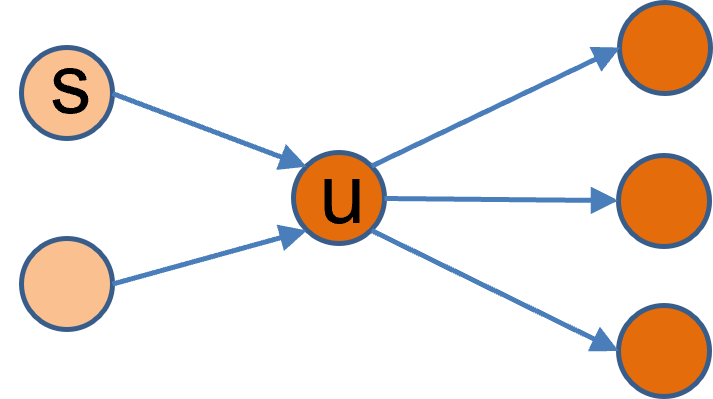
\includegraphics[width=0.35\linewidth]{figures/tracing_tendency.png}
%     \label{fig:tracing_tendency}
%     }
%     \subfigure[Weight pollution]{
%     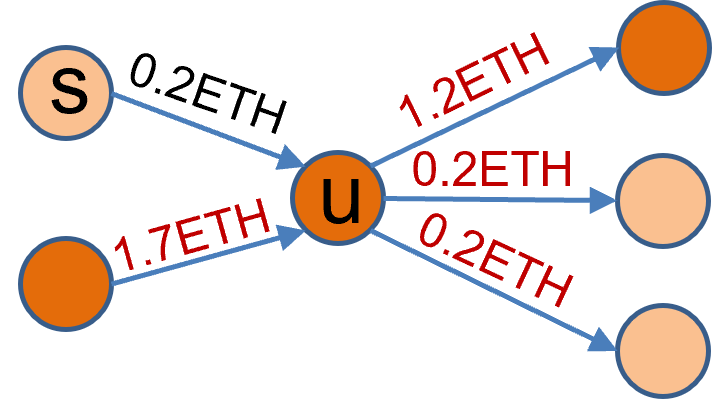
\includegraphics[width=0.35\linewidth]{figures/weight_pollution.png}
%     \label{fig:weight_pollution}
%     }
%     \subfigure[Temporal reasoning]{
%     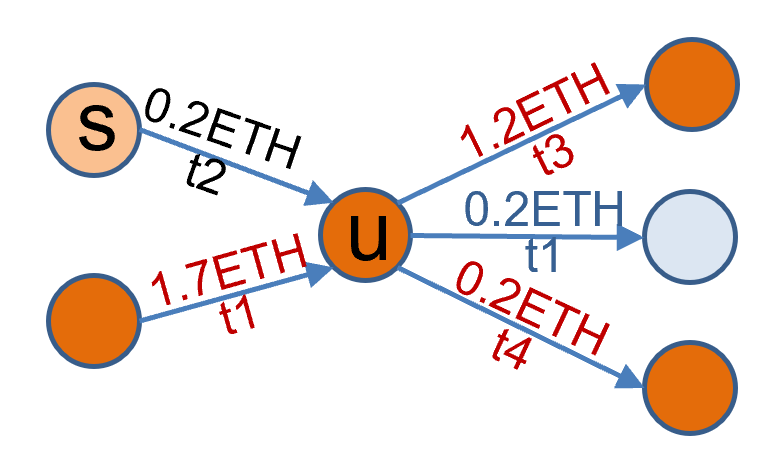
\includegraphics[width=0.35\linewidth]{figures/temporal_reasoning.png}
%     \label{fig:temporal_reasoning}
%     }
%     \subfigure[Token redirection]{
%     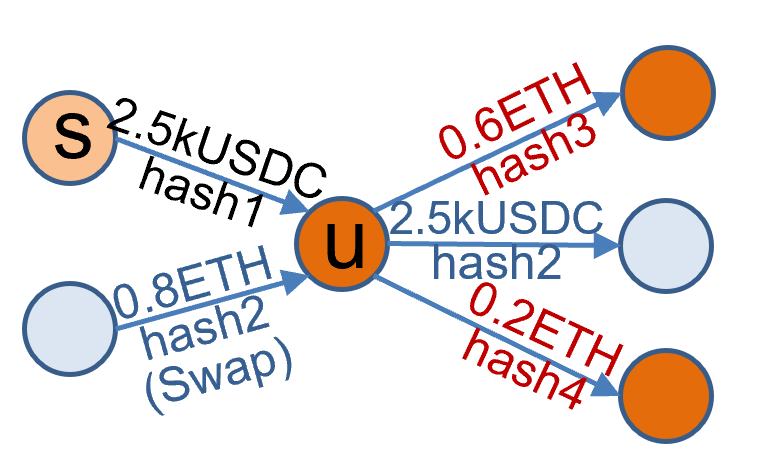
\includegraphics[width=0.35\linewidth]{figures/token_redirection.png}
%     \label{fig:token_redirection}
%     }
%     \caption{
%     (a) Tracing tendency. Different attention is assigned to the out-degree neighbors and in-degree neighbors.
%     (b) Weight pollution. The higher the edge weight, the closer the relationship. 
%     (c) Temporal reasoning. Tracing money flow in chronological order, and $t1<t2<t3<t4$ in this example. 
%     (d) Token redirection. Uncovering the token flow even though there exist complex transaction actions in the Swap pattern.
%     }
% \end{figure}

\textbf{Token redirection}.
% Besides native currency transfers, the transactions of account-based blockchain contain a large number of token transfers, while token redirection makes effort to reveal the real flow of interesting tokens.
This strategy makes the effort to uncover the flow of interesting tokens based on the transaction patterns of Xfer and Swap.
% In TRacer, the transaction patterns of Xfer and Swap are taken into consideration when it comes to tracing the token fund flow.
As Figure \ref{fig:TTR_strategies}(d) shows, the residual of node $u$ brought from the USDC token in an Xfer edge with hash1 should be pushed through the edges with hash3 and hash4, rather than the USDC outgoing edge with hash2. Since the edges with hash2 are in a Swap pattern and swapped the USDC token into ETH.
% As Figure \ref{fig:token_redirection} shows, the residual with USDC token received by the node $u$ in an Xfer edge with hash1 should have been pushed to the out-degree neighbor by the edge with USDC and hash2, but considering the edge with USDC and hash2 for redirection, the residual is pushed through the output edges with hash3 and hash4.
To achieve the redirection of token flows in complex transaction actions, we define a recursive function $\rho(\cdot,\cdot)$ which can find the initial state of a set of incoming edges before the Swap operations and the final state of a set of outgoing edges after the Swap operations within a node. For example, the initial state before Swap of the incoming edge with hash2 in Figure \ref{fig:TTR_strategies}(d) is the incoming edge with hash1, and the final state after Swap of the outgoing edge with hash2 is the outgoing edges with hash3 and hash4. More specifically, as shown in Algorithm \ref{alg:ttr_local_push} line 8-14, the residual of a specific token should be pushed through the redirected edges. Therefore, $\rho(\cdot,\cdot)$ satisfies the following recursive equation:
\begin{equation}\label{equation:token_redirect}
    \rho(\mathcal{E}, E(u))=\mathcal{E}_{xfer} \cup \rho(\bigcup\limits_{e \in \mathcal{E}_{swap}} redirect(e), E(u)),    
\end{equation}
where $\mathcal{E}$ is a set of edges for redirection, $\mathcal{E}_{xfer} \subset \mathcal{E}$ is a set of Xfer edges, $\mathcal{E}_{swap} \subset \mathcal{E}$ is a set of Swap edges, and $redirect(\cdot)$ selects the edges in the token types before/after Swap for incoming/outgoing edges $e \in \mathcal{E}_{swap}$ from edges $E(u)$ related to $u$.
% , which satisfies $f_{src}(e')=f_{src}(e)=u$ or $f_{tgt}(e')=f_{tgt}(e)=u$ for $\forall e' \in redirect(e)$.
% redirect selects the output/input edges from $E(u)$ with the swapped token symbol of the output/input edge $e \in \mathcal{E}_{swap}$.
Especially, $\rho(\emptyset, E(u)) = \emptyset$.

\subsubsection{\textit{Pop} and \textit{Expand}: Greedy Selection}
The \textit{Pop} operation selects a node from the subgraph for the next round expansion iteration, and the \textit{Expand} operation expands from a node by collecting all the related edges of this node.
% The \textit{Pop} operation selects a node with high priority from the subgraph in graph expansion, while \textit{Expand} collects all edges related to the selected node.
% In TRacer, the priority of the nodes is residual, where the node with a higher residual has a greater priority.
Note that the graph expansion in TRacer terminates when the residual of all nodes in the subgraph is below a threshold $\epsilon \in (0,1)$, i.e.,
\begin{equation}
    \max\limits_{u \in V}(\sum\limits_{t \in \Gamma}\sum\limits_{b \in B}r_s(u,t,b)) < \epsilon.
    \label{equ:end_cond}
\end{equation}
Thus we proposed the \textbf{greedy selection} for the \textit{Pop} operation to achieve the condition in Equation \ref{equ:end_cond}, i.e., the \textit{Pop} operation selects the node in the subgraph with the highest residual.
% Thus we proposed two types of node selection rules for the \textit{Pop} operation to achieve the condition in Equation \ref{equ:end_cond}, namely greedy selection, and group selection:
% \begin{itemize}
%     \item \textbf{Greedy selection}: Select one node in the subgraph with the highest residual.
%     \item \textbf{Group selection}: Select all nodes in the subgraph where the residual of every node is greater than $\epsilon$.
% \end{itemize}
% In our implementation, the greedy selection is chosen for \textit{Pop} operation enabled to reduce the pressure of data access in \textit{Expand}.

% \subsection{\textit{Extract}: Local Community Detection}
\subsection{Local Community Detection}
Referring to Figure~\ref{fig:TRacer}, the \textit{Extract} operation employs local community detection to construct a small-scale local community from the expanded graph. For a particular risky source node, the importance rank of the nodes within the local community is significantly higher than the external nodes, making it easy for further expert auditing.


The less conductance \cite{andersen2006local, andersen2007local} of the local community, the higher rank of the nodes in the local community than external nodes, in which the conductance is:
\begin{equation}
    \Phi(S)=\frac{\bm{p}_s(\partial(S))}{\bm{p}_s(S)},
\end{equation}
where $S$ denotes the nodes of the local community, the boundary $\partial(S)=\{ v| (u,v) \in E \land u \in S \land v \in \bar{S} \}$, $\bar{S}$ is the complement of $S$ and $\bm{p}_s(S)=\sum_{u \in S}\bm{p}_s(u)$ denotes the sum of rank over each node in the local community.
Given a specific threshold $\varphi > 0$ for conductance, the local community detection finds the local community satisfying:
\begin{equation}
    \Phi(S) < \varphi.
    \label{equ:local_comm_cond}
\end{equation}
With $S=\{s\}$ as the initialization, Algorithm \ref{alg:ttr_local_comm} describes how to find the local community satisfied the Equation \ref{equ:local_comm_cond}.
\begin{algorithm}[t]
    \caption{TTR-based Local Community Detection}
    \label{alg:ttr_local_comm}
    \begin{algorithmic}[1]
        \REQUIRE The source node $s$, the subgraph of graph expansion $G_s=(V_s, E_s)$, and the TTR score vector $\bm{p}_s$.
        \ENSURE The local community with nodes set $S$.
        \STATE $S = \{ s \}$
        \STATE $\bar{S} = V_s \setminus S$
        \WHILE{$\Phi(S) \geq \varphi$}
            \STATE $u =\mathop{\arg\max}_{v\in\bar{S}}\bm{p}_s(v)$
            % \STATE $u =$ the node with the highest rank in $\bar{S}$
            \STATE $S = S \cup \{ u \}$
            \STATE $\bar{S} = \bar{S} \setminus \{ u \}$
        \ENDWHILE
        \RETURN $G_s.subgraph(S)$
    \end{algorithmic}
\end{algorithm}
\subsection{Theoretical properties}
In this part, we discuss the theoretical properties of TRacer, and prove that our method is able to finish the transaction tracing task in large-scale transaction graphs with a constant time cost. Besides, we discuss the upper limit of the tracing depth in TRacer.

As the description in Proposition \ref{pot:cost}, the cost of TRacer is independent of the graph size, indicating that TRacer is able to trace on the large-scale transaction graph with a low cost.
\begin{proposition}
\label{pot:cost}
The iteration of graph expansion runs $O(\frac{1}{\epsilon \alpha})$ times, and the number of nodes with non-zero values in the output TTR score is at most $O(\frac{1}{\epsilon \alpha})$, which guarantees the cost of local community detection is $O(\frac{1}{\epsilon \alpha})$.
\end{proposition}
\begin{proof}
This follows from Andersen et al. \cite{andersen2006local}, Lemma 2.
\end{proof}

In addition, what depth can TRacer trace in a transaction graph from the source node is described in Proposition \ref{pot:max_depth}.
% where the higher order of the neighbor, the longer distance between the source node and this neighbor.
\begin{proposition}
\label{pot:max_depth}
An $n$-hop neighbor of the source node can be found in the graph obtained by graph expansion, in which $n$ satisfies:
\begin{equation}
    n \leq \frac{log(\epsilon)}{log(1-\alpha)} + 1.
\end{equation}
\end{proposition}
\begin{proof}
In order to maximize the rank of the neighbors far away from the source node, $\alpha$ needs to be as small as possible, and $\beta$ needs to be as close as possible to 0 or 1, which ensures that the residual can be pushed to a specific direction.
Let the sum of residual pushed from the source node $s$ to the $n$-hop neighbors be $r^{(n)}$.
Considering $\beta=1$ here, $r^{(n)}$ can be obtained by:
\begin{equation}
    \begin{cases}
        & r^{(1)}=(1-\alpha), \\
        & r^{(2)} \geq (1-\alpha)(r^{(1)}-k_1 \epsilon)=(1-\alpha)^2-(1-\alpha)k_1 \epsilon, \\
        & ...... \\
        & r^{(n)} \geq (1-\alpha)(r^{(n-1)}-k_{n-1} \epsilon) \\
        & \ \ \ \ \ \ \ \ =(1-\alpha)^n-\sum\limits_{i=1}^{n-1}(1-\alpha)^{n-i}k_{n-i} \epsilon, \\
    \end{cases}
\end{equation}
where $k_i$ represents the number of nodes with residual less than $\epsilon$ in the $i$-order neighbors of the source node.
Therefore, $r^{(n)}$ obtains the maximum value when:
\begin{equation}
    \sum\limits_{i=1}^{n-1}(1-\alpha)^{n-i}k_{n-i} \epsilon = 0,
\end{equation}
which means the residual of each $i$-order node is greater or equal than $\epsilon$. 
This situation exists when the source node is in a path-like graph, whose adjacency matrix $A$ satisfies $A(i,i+1)=1$ and other elements are $0$.
Considering the end condition of the local push procedure, the residual of $n$-hop neighbors is:
\begin{equation}
\begin{cases}
    & (1-\alpha)^n < \epsilon\\
    & (1-\alpha)^{n-1} \geq \epsilon \\
\end{cases}
    % r^{(n)}=(1-\alpha)^n \geq \epsilon
    \Rightarrow 
    \frac{log(\epsilon)}{log(1-\alpha)} < n \leq \frac{log(\epsilon)}{log(1-\alpha)} + 1.
    % n \leq \frac{log(\epsilon)}{log(1-\alpha)}.
\end{equation}
\end{proof}
% ------------ 旧版内容 ------------
% \subsection{Push-Pop Model}
% In this paper, we propose a general framework called Push-Pop model for transaction tracking on blockchain trading systems. 
% As shown in Figure \ref{fig:push_pop_model}, the Push-Pop model starts from the source node $s$ with a specific transaction tracking strategy $T$, builds a witnessed network iteratively, and finds a subgraph from the witnessed network as the local tracking network of the source node finally.
% Here we aim to find a local tracking network containing as many target nodes as possible.
% The witnessed network of a source node under a transaction tracking strategy $T$ is defined as $G_s^T=(V_s^T,E_s^T,PR_s^T)$, where $V_s^T$ and $E_s^T$ denote the nodes and edges of $G_s^T$ respectively while $PR_s^T$ is a vector denoting the priority of all nodes in $G_s^T$.

% To build $G_s^T$ for source node $s$, the steps of Push-Pop model are defined as follows:
% \begin{enumerate}
%     \item \textit{initialize}: Let $V_s^{T}=\{ s \}$, $E_s^{T}=\emptyset$, and $PR_s^T(s)=1$.
%     \item \textit{pop}: Output the node $v$ with the highest priority from the node set $V_s^{T}$.
%     \item \textit{expand}: Query the edges $E(v)$ related to $v$ and the neighbor nodes $N(v)$ of $v$.
%     \item \textit{push}: Update the witnessed network $G_s^T$ in which $E_s^{T}=E_s^{T} \cup E(v)$, $V_s^{T}=V_s^{T} \cup N(v)$, and employ the transaction tracking strategy $T$ to rank the priority of nodes in $V_s^T$ for updating $PR_s^{T}$. If the end condition of $T$ is not satisfies, go to step 2.
%     \item \textit{extract}: Output a subgraph of the witnessed network $G_s^T$ as the local tracking network $G_s$.
% \end{enumerate}

% % Therefore, the Push-Pop model is defined as Algorithm \ref{alg:push_pop}.
% Obviously, the effectiveness of Push-Pop model depends on the transaction tracking strategy, and how to design an effective strategy will be discussed in the next part.
% % \begin{algorithm}[htb]
% %     \caption{Push-Pop Model}
% %     \label{alg:push_pop}
% %     \begin{algorithmic}[1]
% %         \REQUIRE The transaction network $G$, the source node $s$, transaction tracking strategy $T$
% %         \ENSURE The local tracking network captured by $T$
% %         \STATE $T.V.init(s)$
% %         \WHILE{$T.V.hasNext()$}
% %             \STATE $u = T.V.pop()$
% %             \STATE $E(u) = T.expand(u)$
% %             \STATE $T.V.push(E(u))$
% %         \ENDWHILE
% %         \RETURN $T.extract(G_T)$
% %     \end{algorithmic}
% % \end{algorithm}

% \subsection{Transaction Tracking Rank Algorithm}
% The TTR algorithm improves the local push procedure of APPR to enable that nodes related to the source node in a given transaction network $G=(V,E)$ can have a higher estimate of $\bm{p}_s$.
% According to the attributes of transaction network, we design three local push strategies in the TTR algorithm.

% % \begin{figure*}[htb]
% %     \centering
% %     \subfigure[tracking tendency]{
% %         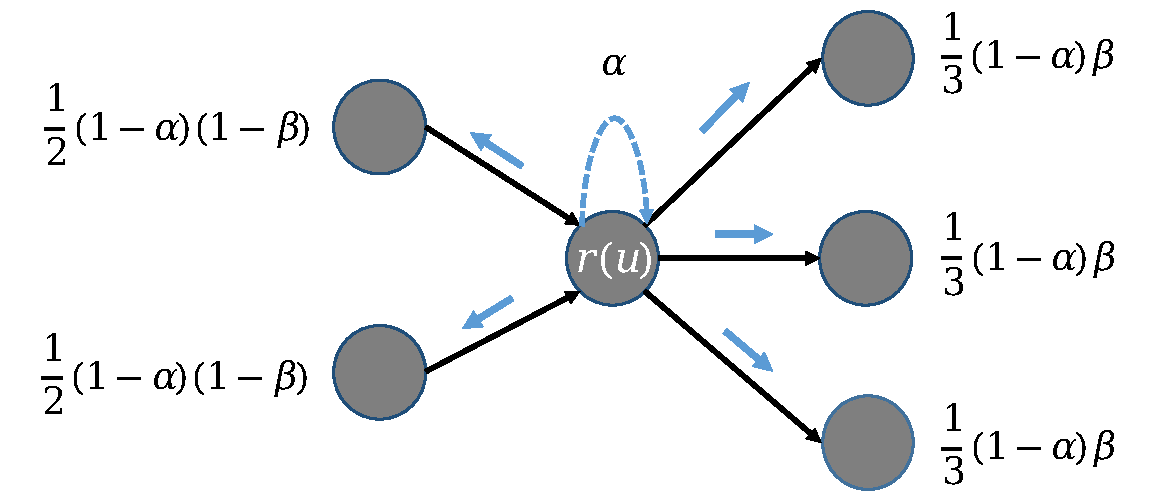
\includegraphics[width=0.3\linewidth]{figures/local_push_ttr_base.pdf}
% %         \label{fig:local_push_ttr_base}
% %     }
% %     \subfigure[weight pollution]{
% %         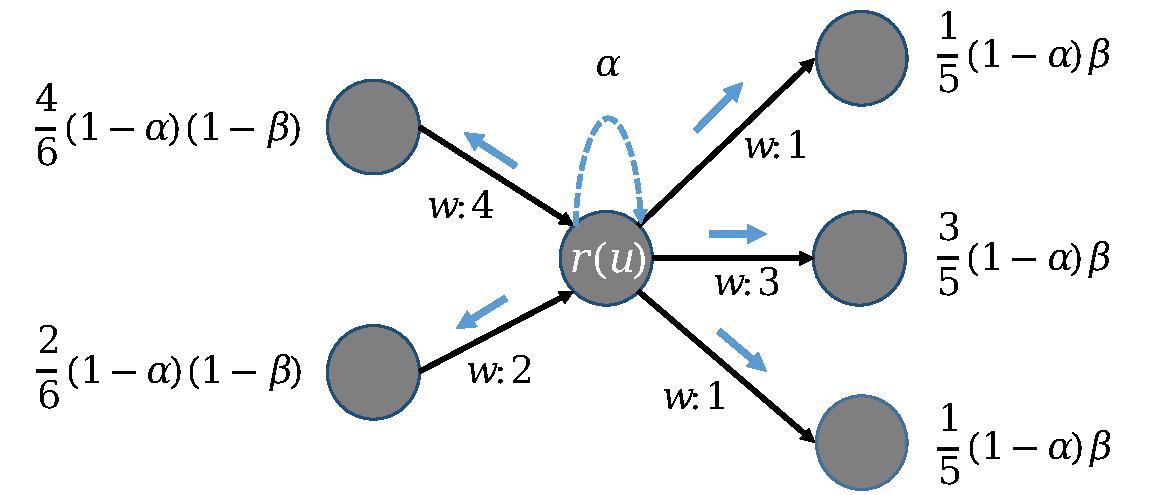
\includegraphics[width=0.3\linewidth]{figures/local_push_ttr_weight.pdf}
% %         \label{fig:local_push_ttr_weight}
% %     }
% %     \subfigure[temporal reasoning]{
% %         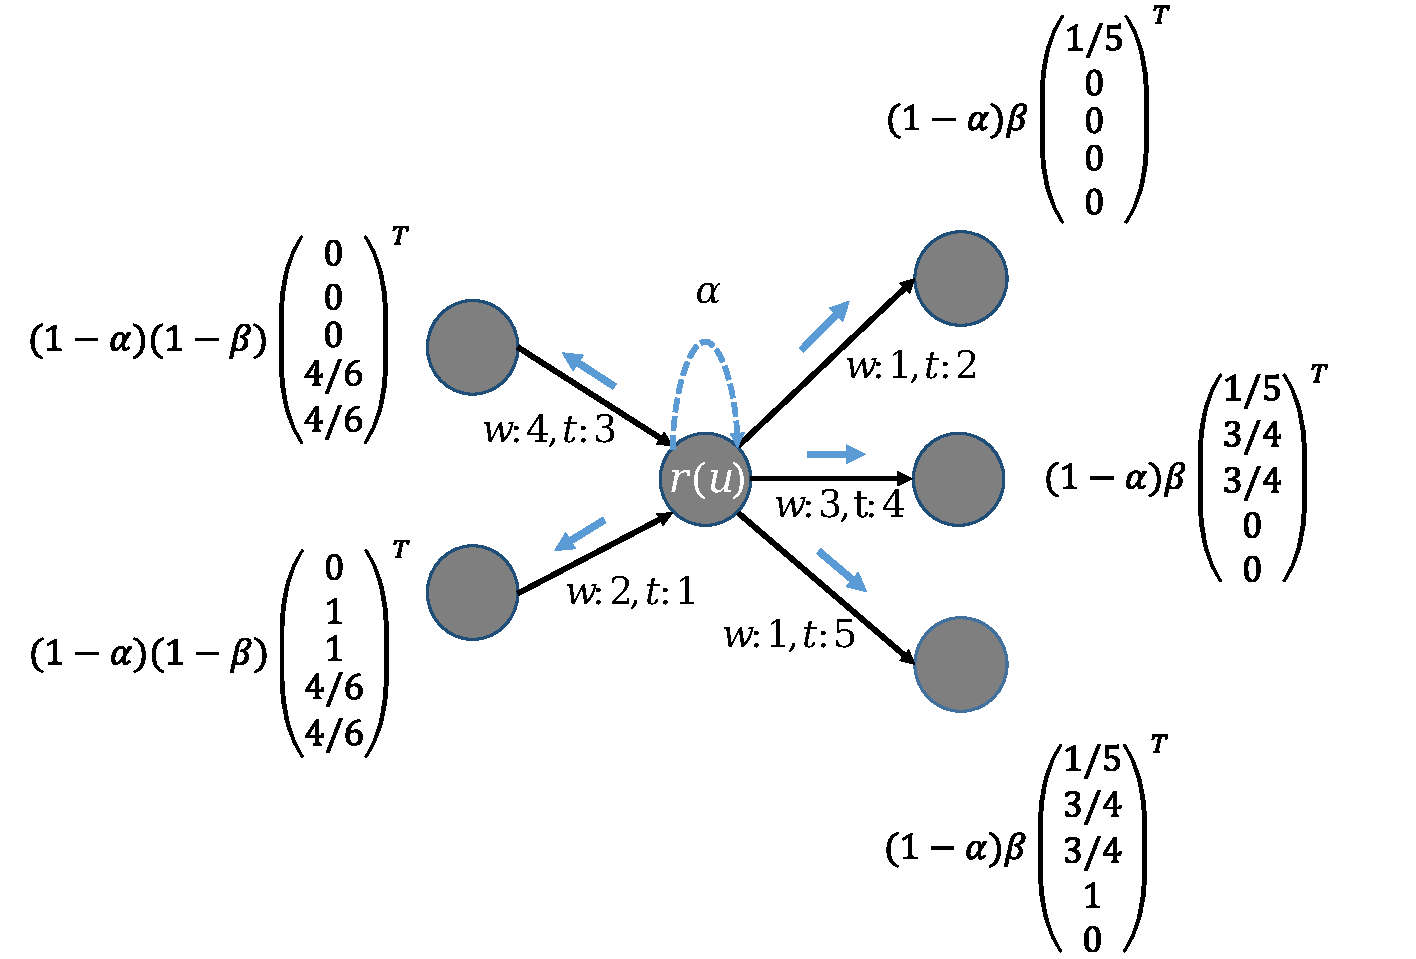
\includegraphics[width=0.3\linewidth]{figures/local_push_ttr_time.pdf}
% %         \label{fig:local_push_ttr_time}
% %     }
% %     \caption{TTR.}
% % \end{figure*}

% % 介绍三种递进的push策略
% \subsubsection{Tracking tendency}
% Since a transaction relationship between addresses is directed, during the transaction tracking process, the attention to in-degree neighbors and out-degree neighbors may be different. 
% For example, tracking for the target of the fund flows oriented from a particular needs to pay more attention to its out-degree neighbors, while searching for the source of money needs to pay more attention to the in-degree neighbors.
% Therefore, considering the transaction network $G$ as a directed graph and giving a tracking tendency coefficient $\beta \in [0,1]$, the out-degree neighbors in a transaction relationship can get a higher estimate of $\bm{p}_s$ when $\beta > 0.5$, and the in-degree neighbors in a transaction relationship can get a higher estimate of $\bm{p}_s$ when $\beta < 0.5$.
% % The local push procedure can push the residual to self, out-degree neighbors, and in-degree neighbors with different ratios.
% In this way, Equation \ref{equ:ppr} can be re-written as:
% \begin{equation}
%     \bm{p}_s = \alpha \bm{e}_s + (1-\alpha) \bm{p}_s M_{\beta}.
%     \label{equ:ttr_base}
% \end{equation}
% The transition matrix of Equation \ref{equ:ttr_base} is:
% \begin{equation}
%     M_{\beta} = \beta D_{out}^{-1}A + (1-\beta)D_{in}^{-1}A^T,
% \end{equation}
% where $A$ is the adjacency matrix of $G$, $D_{out}$ is an out-degree matrix of $G$, and $D_{in}$ is an in-degree matrix of $G$.

% In this way, the local push procedure of node $u$ pushes the residual to itself, out-degree neighbors, and in-degree neighbors. 
% And each in-degree neighbor and each out-degree neighbor receive an equal proportion depending on the in-degree and out-degree, respectively.
% Therefore, Equations \ref{equ:local_push_appr} can be re-written as:
% \begin{equation}
%     \begin{cases}
%         & \bm{p}_s(u)=\bm{p}_s(u)+\alpha \bm{r}_s(u) \\ 
%         & \bm{r}_s(v_{out})=\bm{r}_s(v_{out})+\theta_{\beta}(u,v_{out}) \bm{r}_s(u) \\ 
%         & \bm{r}_s(v_{in})=\bm{r}_s(v_{in})+\theta_{\beta}(u,v_{in}) \bm{r}_s(u)
%     \end{cases},
%     \label{equ:local_push_ttr_base}
% \end{equation}
% where $v_{out} \in N_G^{out}(u)$ and $v_{in} \in N_G^{in}(u)$ denote out-degree neighbor and in-degree neighbor of $u$ respectively, and the push factors are defined as follows:
% \begin{equation}
%     \theta_{\beta}(u,v_{out})=\frac{(1-\alpha)\beta}{d_{out}(u)},
% \end{equation}
% \begin{equation}
%     \theta_{\beta}(u,v_{in})=\frac{(1-\alpha)(1-\beta)}{d_{in}(u)},
% \end{equation}
% in which $d_{out}(u)$ and $d_{in}(u)$ denote out-degree and in-degree of $u$ respectively.
% % \begin{figure}[htb]
% %     \centering
% %     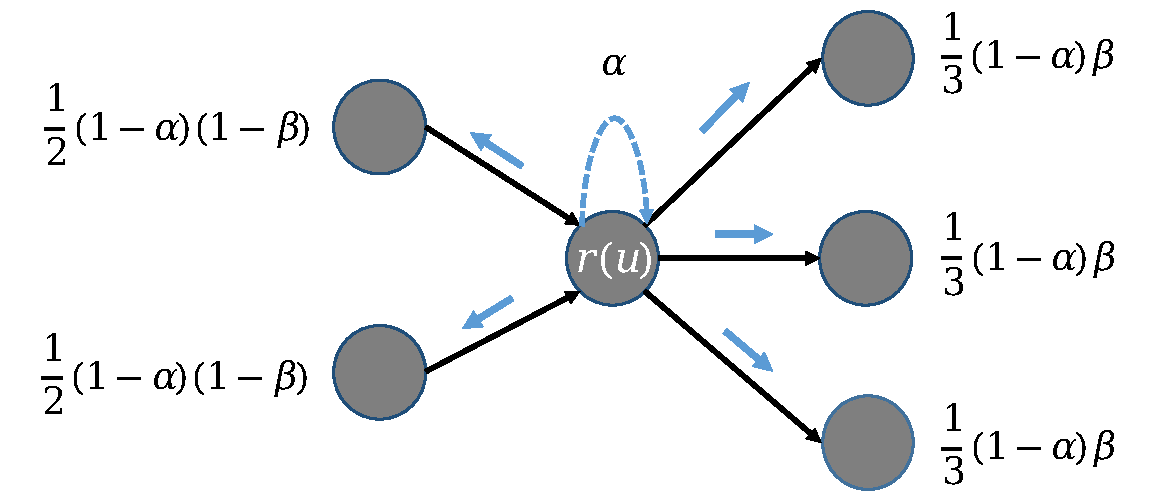
\includegraphics[width=\linewidth]{figures/local_push_ttr_base.pdf}
% %     \caption{Local push procedure with tracking tendency}
% %     \label{fig:local_push_ttr_base}
% % \end{figure}
% And if a node $u$ has no out-degree neighbors or in-degree neighbors, the residual can be pushed to itself.
% % \begin{equation}
% %     r(u)=r(u)+(1-\alpha)\beta r(u),
% % \end{equation}
% % \begin{equation}
% %     r(u)=r(u)+(1-\alpha)(1-\beta) r(u).
% % \end{equation}


% \subsubsection{Weight pollution}
% Traditional APPR pushes the residual of a node to the neighbors by considering an equal weight during a local push iteration. However, in a transaction relationship, the transaction strength is usually weighted by the transaction amount. For each node in the network, a neighbor who has transaction relationships with a larger amount of money is considered to be more relevant to the node. 
% % For example, tracking the fund flow of a node $u$ needs to pay more attention to the neighbors having a large amount of transactions related to $u$.
% % In the procedure of transaction tracking, attention to the nodes whether related to the source node on the amount is needed.
% % For example, the amount received by some nodes is similar to the amount output by the source node, these nodes may be related to the source node.
% Therefore, by considering the transaction network $G$ as a weighted directed graph with the transaction amount information as the weight, Equation \ref{equ:ttr_base} can be re-written as:
% %the nodes get a higher estimate of $\bm{p}_s$ when these nodes have a significant association with the source node on the perspective of edge weight.
% \begin{equation}
%     \bm{p}_s = \alpha \bm{e}_s + (1-\alpha) \bm{p}_s M_w.
%     \label{equ:ttr_weight}
% \end{equation}
% The transition matrix of Equation \ref{equ:ttr_weight} is:
% \begin{equation}
%     % M_w = \beta {D_{out}^w}^{-1}W + (1-\beta){D_{in}^w}^{-1}W^T,
%     M_w = \beta \tilde{D}_{out}^{-1}W + (1-\beta)\tilde{D}_{in}^{-1}W^T,
% \end{equation}
% where $W$ is the weighted adjacency matrix of $G$, $\tilde{D}_{out}$ is the weighted out-degree matrix of $G$, $\tilde{D}_{in}$ is the weighted in-degree matrix of $G$. 
% The diagonal elements of $\tilde{D}_{out}$ and $\tilde{D}_{in}$ are defined as follows:
% \begin{equation}
%     \tilde{D}_{out}(i,i)=||W(i,)||,
% \end{equation}
% \begin{equation}
%     \tilde{D}_{in}(i,i)=||W^T(i,)||, i\leq|V|
% \end{equation}
% where $W(i,)$ and $W^T(i,)$ denote the $i$-th row in $W$ and $W^T$ respectively. All off-diagonal elements in $\tilde{D}_{out}$ and $\tilde{D}_{in}$ equal to 0.

% In this way, the local push procedure of node $u$ pushes residual to itself, the out-degree neighbors and the in-degree neighbors with different ratios determined by edge weight. And Equations \ref{equ:local_push_ttr_base} can be re-written as:
% % \begin{equation}
% %     \begin{cases}
% %       & p(u)=p(u)+\alpha r(u), \\ 
% %       & r(\hat{v})=r(\hat{v})+(1-\alpha)\beta \frac{W(u,\hat{v})}{W(u,)} r(u), \\ 
% %       & r(\tilde{v})=r(\tilde{v})+(1-\alpha)(1-\beta) \frac{W(\tilde{v},u)}{W(,u)} r(u),
% %     \end{cases}
% % \end{equation}
% \begin{equation}
%     \begin{cases}
%       & \bm{p}_s(u)=\bm{p}_s(u)+\alpha \bm{r}_s(u) \\ 
%       & \bm{r}_s(v_{out})=\bm{r}_s(v_{out})+\theta_w(u,v_{out}) \bm{r}_s(u) \\ 
%       & \bm{r}_s(v_{in})=\bm{r}_s(v_{in})+\theta_w(u,v_{in}) \bm{r}_s(u)
%     \end{cases},
%     \label{equ:local_push_weight}
% \end{equation}
% where the push factors are defined as follows:
% \begin{equation}
%     \theta_w(u,v_{out})=(1-\alpha)\beta\frac{w(u,v_{out})}{\tilde{d}_{out}(u)},
% \end{equation}
% \begin{equation}
%     \theta_w(u,v_{in})=(1-\alpha)(1-\beta)\frac{w(v_{in},u)}{\tilde{d}_{in}(u)},
% \end{equation}
% in which $w(u,v)$ for $\forall{u,v \in V}$ denotes the transaction amount from $u$ to $v$, and $\tilde{d}_{out}(u)$ and $\tilde{d}_{in}(u)$ denote the weighted out-degree and weighted in-degree of $u$ respectively.
% % \begin{figure}[htb]
% %     \centering
% %     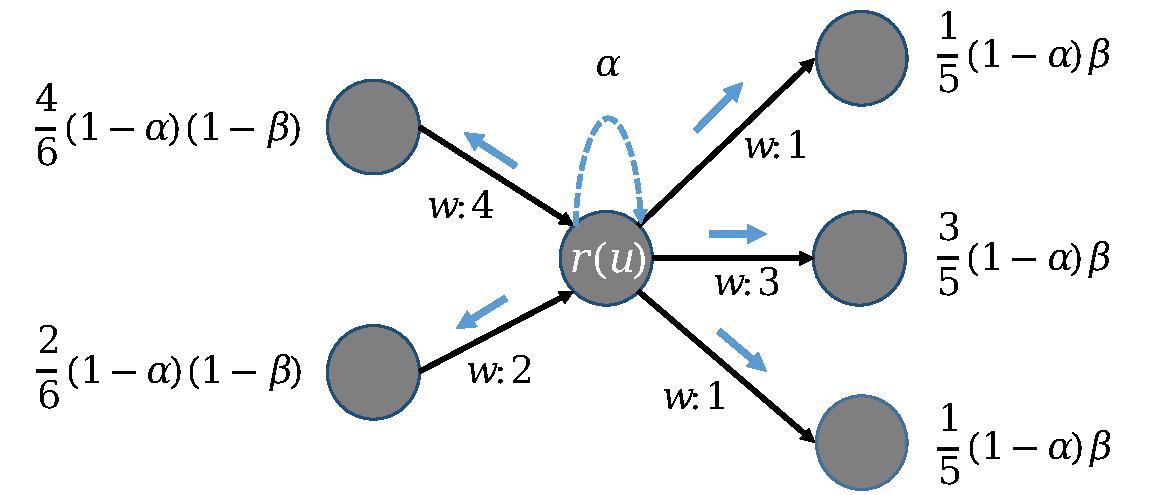
\includegraphics[width=\linewidth]{figures/local_push_ttr_weight.pdf}
% %     \caption{Local push procedure with weight pollution}
% %     \label{fig:local_push_ttr_weight}
% % \end{figure}

% \subsubsection{Temporal reasoning} Blockchain transactions are recorded in blocks chronologically, and each block contains a specific timestamp. Since the fund flow transferring process is dynamic, the transaction time information can be taken into consideration in the local push procedure.
% % Since a transaction relationship is temporal, during the transaction tracking process, the attention to the neighbors may be different.
% In the scenario of blockchain transaction tracking, tracking for the target of a fund flow usually follows the paths with increasing timestamps, while tracking back to the source of a fund flow follows the paths with decreasing timestamps.
% % In the procedure of transaction tracking, starting from the source node, the nodes in the increasing timestamp fund flow or decreasing timestamp fund flow get higher importance.
% % Therefore, considering the transaction network $G$ as a temporal weighted directed graph in which $G^{(t)}$ denotes the weighted directed graph at the $t$-th timestamp, for all timestamp indices $\{1,2, ...,t, ..., t_{\rm max} \}$
% % in $G$, Equation \ref{equ:ttr_weight} can be re-written as:
% Therefore, considering the transaction network $G$ as a temporal weighted directed graph in which $G^{(t)}$ denotes the weighted directed graph at timestamp $t$, for all timestamp $\{ t_1,...,t_k,...,t_n \}$ in $G$, Equation \ref{equ:ttr_weight} can be re-written as:
% \begin{equation}
%     \bm{p}_s^{(t)} = \alpha \bm{e}_s^{(t)} + (1-\alpha) p_s^{(t)} M_w^{(t)},
%     \label{equ:ttr}
% \end{equation}
% where $\bm{p}_s^{(t)}$ denotes the estimate of $\bm{p}_s$ at timestamp $t$, $M_w^{(t)}$ denotes the transition matrix at timestamp $t$, and $\bm{e}_s^{(t)}$ denotes the indicator vector at timestamp $t$ in which $\bm{e}_s^{(t_1)}=\bm{e_s}$ and $\bm{e}_s^{(t_k)} = \bm{p}_s^{(t_{k-1})}$.
% % where $P_s$ is a $t_{max} \times |V|$ matrix in which each row $P_s(t,)$ denotes the importance of all nodes to the source node at $t$-th timestamp.
% % element $\bm{P}_s^{(t)}(u)$ is able to describe the importance of node $u$ to the source node at time $t$
% In this case, $\bm{p}_s$ is redefined as follow:
% \begin{equation}
%     % \bm{p}_s=\sum\limits_{t=1}^{t_{\rm max}}{P_s(t,)}.
%     \bm{p}_s=\frac{1}{n}\sum\limits_{t{'}=t_1}^{t_n}{\bm{p}_s^{(t{'})}}.
% \end{equation}
% % , and the estimate of $p$ can be re-written as $p=\sum_t{p_{\infty}^{(t)}}$.
% The transition matrix of Equation \ref{equ:ttr} is:
% \begin{equation}
%     % M_{t} = \beta \hat{D}_{out}^{-1}W_{t} + (1-\beta)\hat{D}_{in}^{-1}W_{t}^T,
%     % M_{T} = \beta \hat{D}_{out}^{-1}\mathcal{W} + (1-\beta)\hat{D}_{in}^{-1}\mathcal{W}^T,
%     M_{w}^{(t)} = \beta \hat{D}_{out}^{{(t)}^{-1}} W^{(t)} + (1-\beta)\hat{D}_{in}^{{(t)}^{-1}} W^{{(t)}^T},
% \end{equation}
% where $W^{(t)}$ is a weighted adjacency matrix at timestamp $t$, $\hat{D}_{out}^{(t)}$ and $\hat{D}_{in}^{(t)}$ denote the cumulative weighted out-degree matrix and the cumulative weighted in-degree matrix at timestamp $t$ respectively.
% % where $\mathcal{W}$ is a $t_{\rm max} \times |V| \times |V|$ tensor in which $\mathcal{W}(t,)$ denotes the weighted adjacency matrix at the $t$-th timestamp, $\hat{D}_{out}$ and $\hat{D}_{in}$ record the weighted out-degree matrix and the weighted in-degree matrix in each timestamp respectively with the same dimension as $\mathcal{W}$. 
% % $\hat{D}_{out}$ is a temporal weighted out-degree matrix of $G$, 
% % $\hat{D}_{in}$ is a temporal weighted in-degree matrix of $G$, 
% % and $\hat{D}_{out}$ and $\hat{D}_{in}$ have the same dimensions as $W_{t}$.
% The nonzero elements of $\hat{D}_{out}$ and $\hat{D}_{in}$ are defined as follows:
% \begin{equation}
%     % \hat{D}_{out}(t,i,i)=\sum\limits_{t{'}>t}||\mathcal{W}(t',i,)||,
%     \hat{D}_{out}^{(t)}(i,i)=\sum\limits_{t{'}\leq t}||W^{(t{'})}(i,)||,
% \end{equation}
% \begin{equation}
% %   \hat{D}_{in}(t,i,i)=\sum\limits_{t{'}<t}||\mathcal{W}^T(t',i,)||, t\leq t_{\rm max}, i\leq|V|,
%     \hat{D}_{in}^{(t)}(i,i)=\sum\limits_{t{'}\geq t}||W^{(t{'})}(,i)||, t_1 \leq t\leq t_{n}, i\leq|V|,
% \end{equation}
% in which $W^{(t{'})}(i,)$ and $W^{(t{'})}(,i)$ denote the $i$-th row and the $i$-th column in the weighted adjacency matrix at timestamp $t{'}$ respectively.
% % Especially, $\hat{D}_{out}=\tilde{D}_{out}$ and $\hat{D}_{in}=\tilde{D}_{in}$ at timestamp $t_1$.
% % in which $\mathcal{W}(t,i,)$ denotes the row $i$ in the weighted adjacency matrix at the $t$-th timestamp respectively.
% % \begin{equation}
% %     \hat{D}_{t}(i,j,j)=\hat{d}_{t}^{(t_i)}(v_j)=\sum\limits_{t{'}>t}||W_{t}(i,j)||,
% % \end{equation}
% % \begin{equation}
% %   \tilde{D}_{t}(i,j,j)=\tilde{d}_{t}^{(t_i)}(v_j)=\sum\limits_{t{'}<t}||W_{t}^T(i,j)||,
% % \end{equation}
% % in which $W_{t}(i,j)$ and $W_{t}^T(i,j)$ denote the rows $j$ in $W_{t}$ and $W_{t}^T$ at timestamp $t_i$ respectively.

% In this way, the local push procedure of node $u$ pushes the residual to itself, out-degree neighbors, and in-degree neighbors with different ratios determined by the transaction amount and time.
% Equations \ref{equ:local_push_weight} can be re-written as:
% % \begin{equation}
% %     \begin{cases}
% %       & \bm{p}_s(u)=\bm{p}_s(u)+\alpha \bm{e} \cdot R_s(u), \\ 
% %       & R_s(\hat{v})=R_s(\hat{v})+\theta_{t}(u,\hat{v}) \odot R_s(u), \\ 
% %       & R_s(\tilde{v})=R_s(\tilde{v})+\theta_{t}(u,\tilde{v}) \odot R_s(u),
% %     \end{cases}
% % \end{equation}
% \begin{equation}
%     \begin{cases}
%       & \bm{p}_s(u)=\bm{p}_s(u)+\alpha \bm{e} \cdot R_s(u) \\ 
%       & R_s(v_{out})=R_s(v_{out})+\theta_{t}(u,v_{out}) \odot R_s(u) \\ 
%       & R_s(v_{in})=R_s(v_{in})+\theta_{t}(u,v_{in}) \odot R_s(u)
%     \end{cases},
% \end{equation}
% where $R_s$ denotes a $n \times |V|$ matrix in which $R_s(v_i)=R_s(,i)$ denotes the residual of a node $v_i$ at each timestamp, $\odot$ denotes the element-wise product, and the push factors are defined as follows:
% % where $R_s$ denotes a $n \times |V|$ matrix in which $R_s(v_i)=R_s(,i)$ denotes the residual of a node $v_i$ at each timestamp, $\odot$ denotes the element-wise product, and the push factors are defined as follows:
% % \begin{equation}
% %     \theta_{t}(u,\hat{v})=(1-\alpha)\beta w_{t}(u,\hat{v}) \oslash \hat{d}_{t}(u),
% % \end{equation}
% % \begin{equation}
% %     \theta_{t}(u,\tilde{v})=(1-\alpha)(1-\beta) w_{t}(\tilde{v},u) \oslash \tilde{d}_{t}(u),
% % \end{equation}
% \begin{equation}
%     \theta_{t}(u,v_{out})=(1-\alpha)\beta w_{t}(u,v_{out}) \oslash \hat{d}_{out}(u),
% \end{equation}
% \begin{equation}
%     \theta_{t}(u,v_{in})=(1-\alpha)(1-\beta) w_{t}(v_{in},u) \oslash \hat{d}_{in}(u),
% \end{equation}
% in which $w_{t}(u,v)$ for $\forall{u,v \in V}$ is a vector denoting the transaction amount from $u$ to $v$ at each timestamp, $\hat{d}_{out}(u)$ and $\hat{d}_{in}(u)$ denote the temporal weight out-degree and in-degree at each timestamp respectively, and $\oslash$ denotes the element-wise division.

% Based on the above local push strategies, we propose the TTR algorithm.
% Giving a transactions network $G=(V,E)$, TTR tracking for the target starting from the source node $s$.
% Initializing $R_s$ with edges related to $s$, TTR calls the local push procedure to push the residual for a node itself, the out-degree neighbors, and the out-degree neighbors by ``selfPush", ``forwardPush" and ``backwardPush"  procedure respectively, until the residual of each node is within the minimum error $\epsilon$.
% % initializes the estimate $p=\vec{0}$ and the temporal residual $r_{\infty}$, and then 
% % call the local push procedure to push the residual for self, out-degree neighbors and out-degree neighbors by ``selfPush", ``forwardPush" and ``backwardPush"  procedure respectively, until the residual of each node within the minimum error $\epsilon$.
% Algorithm \ref{alg:ttr} describes the framework of the TTR algorithm, Algorithm \ref{alg:self_push}, Algorithm \ref{alg:forward_push} and Algorithm \ref{alg:backward_push} describe the ``selfPush", ``forwardPush" and ``backwardPush" procedure in detail respectively.
% \begin{algorithm}[t]
%     \caption{Transaction Tracking Rank}
%     \label{alg:ttr}
%     \begin{algorithmic}[1]
%         \REQUIRE Source node $s$, transactions network $G=(V,E)$ with timestamp range $\{t_1,t_2,...,t_n\}$, teleport constant $\alpha$, minimum error $\epsilon$, and tracking tendency coefficient $\beta$.
%         \ENSURE the estimate of $\bm{p}_s$
%         \STATE $\bm{p}_s(s)=\alpha$
%         \STATE $R_{s}(t,v)=(1-\alpha)\beta w/\tilde{d}_{out}(s)$ for $\forall{(s,v,w,t)} \in E_{out}(s)$
%         \STATE $R_{s}(t,v)=(1-\alpha)(1-\beta) w/\tilde{d}_{in}(s)$ for $\forall{(v,s,w,t)} \in E_{in}(s)$
%         \IF{$E_{out}(s)=\emptyset$}
%             \STATE $R_s(t_1,s)=(1-\alpha)\beta$
%         \ENDIF
%         \IF{$E_{in}(s)=\emptyset$}
%             \STATE $R_s(t_n,s)=(1-\alpha)(1-\beta)$
%         \ENDIF
%         \WHILE{$||R_s(u)|| \geq \epsilon, u \in V$}
%             \STATE Let $R_s^{\prime}=R_s$, and $R_{s}(u)=\vec{0}$.
%             \STATE Apply $R_s^{\prime}$ to update $\bm{p}_s$ and $R_s$ through selfPush, forwardPush and backwardPush.  
%         \ENDWHILE
%         \RETURN $\bm{p_s}$
%     \end{algorithmic}
% \end{algorithm}

% \begin{algorithm}[t]
%     \caption{selfPush}
%     \label{alg:self_push}
%     \begin{algorithmic}[1]
%         \REQUIRE Node $u$, temporal residual $R_s^{\prime}$, estimate $\bm{p}_s$, and teleport constant $\alpha$.
%         \FOR{$t \in [t_1, t_n]$}
%             \STATE $\bm{p}_s(u)+=\alpha R_s^{\prime}(t,u)$
%         \ENDFOR
%     \end{algorithmic}
% \end{algorithm}

% \begin{algorithm}[t]
%     \caption{forwardPush}
%     \label{alg:forward_push}
%     \begin{algorithmic}[1]
%         \REQUIRE Node $u$, out-edges $E_{out}(u)$, temporal residual $R_s^{\prime}$ and $R_s$, teleport constant $\alpha$, and tracking tendency coefficient $\beta$.
%         \FOR{$\forall{e:(u,v,w,t)} \in E_{out}(u)$}
%             \STATE $\Delta = 0$
%             \FOR{$\tau \in [t_1,t]$}
%                 \STATE $\Delta += w R_s^{\prime}(\tau,u) / \hat{d}_{out}^{(\tau)}(u)$
%                 % \STATE $\Delta += w{\rho}_{\infty}^{(\tau)}(u) / \hat{d}_{\infty}^{(\tau)}(u)$
%             \ENDFOR
%             % \STATE $r^{(t)}_{\infty}(\hat{v})+=(1-\alpha) \beta \Delta$
%             \STATE $R_s(t,v) += (1-\alpha)\beta \Delta$
%         \ENDFOR
%         \STATE Calculate $max(t)$ from all $t$ in $E_{out}(u)$.
%         \FOR{$\tau \in [max_t, t_n]$}
%             % \STATE $r_{\infty}^{(\tau)}(u)+=(1-\alpha)\beta {\rho}_{\infty}^{(\tau)}(u)$
%             \STATE $R_s(\tau,u) += (1-\alpha)\beta R_s^{\prime}(\tau,u)$
%         \ENDFOR
%     \end{algorithmic}
% \end{algorithm}

% \begin{algorithm}[t]
%     \caption{backwardPush}
%     \label{alg:backward_push}
%     \begin{algorithmic}[1]
%         \REQUIRE Node $u$, in-edges $E_{in}(u)$, temporal residual $R_s^{\prime}$ and $R_s$, teleport constant $\alpha$, and tracking tendency coefficient $\beta$.
%         \FOR{$\forall e:(v,u,w,t) \in E_{in}(u)$}
%             \STATE $\Delta = 0$
%             \FOR{$\tau \in [t, t_n]$}
%                 % \STATE $\Delta += w{\rho}_{\infty}^{(\tau)}(u) / \tilde{d}_{\infty}^{(\tau)}(u)$
%                 \STATE $\Delta += w R_s^{\prime}(\tau, u) / \hat{d}_{in}^{(\tau)}(u)$
%             \ENDFOR
%             % \STATE $r_{\infty}^{(t)}(\tilde{v}) += (1-\alpha)(1-\beta)\Delta$
%             \STATE $R_s(t,v) += (1-\alpha)(1-\beta)\Delta$
%         \ENDFOR
%         \STATE Calculate $min(t)$ from all $t$ in $E_{in}(u)$.
%         \FOR{$\tau \in [t_1, min(t)]$}
%             % \STATE $r_{\infty}^{(\tau)}(u)+=(1-\alpha)(1-\beta) {\rho}_{\infty}^{(\tau)}(u)$
%             \STATE $R_s(\tau,u)+=(1-\alpha)(1-\beta) R_s^{\prime}(\tau,u)$
%         \ENDFOR
%     \end{algorithmic}
% \end{algorithm}

% % \begin{algorithm}[htb]
% %     \caption{forwardPush}
% %     \label{alg:forward_push}
% %     \begin{algorithmic}[1]
% %         \REQUIRE node $u$, out-edges set of node $E(u,)$, residual vector $r$, tracking tendency coefficient $\alpha$ and $\beta$.
% %         \STATE // sort $E(u,)$ and $r(u)$ by timestamp increasingly
% %         \STATE $E(u,)=sort(E(u,))$ 
% %         \STATE $r(u)=sort(r(u))$

% %         \STATE // calcuate sum of weight after each chips
% %         \STATE $j=|E(u,)|-1,w=0,W=mapping$
% %         \FOR{$i \in |r(u)|,|r(u)|-1,...,0$}
% %             \STATE $c=r(u)^i$
% %             \WHILE{$j \geq 0 \wedge E(u,)_t^j > c_t$}
% %                 \STATE $w = w + E(u,)_w^j$
% %                 \STATE $j = j - 1$
% %             \ENDWHILE
% %             \STATE $W(c)=w$
% %         \ENDFOR
        
% %         \STATE // propagate residual weight to outdegree heighbors
% %         \STATE $j=0,d=0$
% %         \FOR{$i \in 0,1,...,|E(u,)|$}
% %             \STATE $e=E(u,)^i$
% %             \WHILE{$j < |r(u)| \wedge e_t > r(u)_t^j$}
% %                 \IF{$W(r(u)^j) > 0$}
% %                     \STATE $d = d + \frac{r(u)_w^j}{W(r(u)^j)}$
% %                 \ENDIF
% %                 \STATE $j = j + 1$
% %                 \STATE $r(e_v)_t=r(e_v)_t + (1-\alpha)\beta e_w d$
% %             \ENDWHILE
% %         \ENDFOR
        
% %         \STATE // not propagated residual weight will back to node $u$
% %         \WHILE{$ j < |r(u)| $}
% %             \STATE $r(u) = r(u) \cup (r(u)_t^j, (1-\alpha)\beta r(u)_w^j)$
% %             \STATE $j=j+1$
% %         \ENDWHILE
% %     \end{algorithmic}
% % \end{algorithm}

% % \begin{algorithm}[htb]
% %     \caption{backwardPush}
% %     \label{alg:backward_push}
% %     \begin{algorithmic}[1]
% %         \REQUIRE node $u$, in-edges set of node $E(,u)$, residual vector $r$, tracking tendency coefficient $\alpha$ and $\beta$.
% %         \STATE // sort $E(,u)$ and $r(u)$ by timestamp increasingly
% %         \STATE $E(,u)=sort(E(,u))$ 
% %         \STATE $r(u)=sort(r(u))$

% %         \STATE // calcuate sum of weight after each chips
% %         \STATE $j=0,w=0,W=mapping$
% %         \FOR{$i \in 0,1,...,|r(u)|$}
% %             \STATE $c=r(u)^i$
% %             \WHILE{$j < |E(,u)| \wedge E(,u)_t^j < c_t$}
% %                 \STATE $w = w + E(,u)_w^j$
% %                 \STATE $j = j + 1$
% %             \ENDWHILE
% %             \STATE $W(c)=w$
% %         \ENDFOR
        
% %         \STATE // propagate residual weight to indegree heighbors
% %         \STATE $j=|r(u)|-1,d=0$
% %         \FOR{$i \in |E(,u)|,|E(,u)|-1,...,0$}
% %             \STATE $e=E(u)^i$
% %             \WHILE{$j \geq 0 \wedge e_t < r(u)_t^j$}
% %                 \IF{$W(r(u)^j) > 0$}
% %                     \STATE $d = d + \frac{r(u)_w^j}{W(r(u)^j)}$
% %                 \ENDIF
% %                 \STATE $j = j - 1$
% %                 \STATE $r(e_v)_t=r(e_v)_t + (1-\alpha)(1-\beta) e_w d$
% %             \ENDWHILE
% %         \ENDFOR
        
% %         \STATE // not propagated residual weight will back to node $u$
% %         \WHILE{$ j \geq 0 $}
% %             \STATE $r(u) = r(u) \cup (r(u)_t^j, (1-\alpha)(1-\beta) r(u)_w^j)$
% %             \STATE $j=j-1$
% %         \ENDWHILE
% %     \end{algorithmic}
% % \end{algorithm}

% Here are some useful theorems (also see \cite{andersen2006local}) to describe the cost of TTR algorithm, and the proofs  given in appendices. 

% \begin{theorem}
% \label{thm:run_time}
% Line 10-line 13 in Algorithm \ref{alg:ttr}, runs in $O(\frac{1}{\epsilon \alpha})$ time, and the number of nodes with non-zero values in the output TTR vector is at most $O(\frac{1}{\epsilon \alpha})$.
% \end{theorem}


% \begin{theorem}
% \label{thm:push_cost}
% The cost of local push procedure including selfPush, forwardPush and backwardPush is $O(|E(u)|log(|E(u)|)$.
% \end{theorem}


% \subsection{TTR-based Push-Pop Model}
% The TTR-based Push-Pop model uses the TTR algorithm as the transaction tracking strategy, which can track the fund flow of the source node $s$ in a transaction network, calculate the relevance between other nodes in the network and the source node, and output a local tracking network.

% For initialization, the TTR-based Push-Pop model set $V_s^T=\{s\}$, and then calls \textit{pop}, \textit{expand}, and \textit{push} in turns until $||R_s(u)|| < \epsilon$ for $\forall{u \in V_s^T}$.
% Finally, the TTR-based Push-Pop model calls \textit{extract} for outputting a local tracking network.
% % The TTR-based Push-Pop model can be described as Algorithm \ref{alg:ttr_based_push_pop}, and
% % where the TTR Strategy maintains all parameters of TTR Algorithm \ref{alg:ttr} like $\epsilon$, and the witnessed graph $G_T=(V_T, E_T)$.
% % the witnessed nodes $V_T$, and the witnessed edges $E_T$.
% The procedures of the TTR strategy in TTR-based Push-Pop model are as follows:
% \begin{itemize}
%     \item \textit{expand}: Query the related edges for a given node $u$. 
%     % Refer to line 4 of Algorithm \ref{alg:ttr_based_push_pop}.
%     \item \textit{push}: The TTR strategy receives a series of edges related to a node $u$ for updating the witnessed network $G_s^T$, and calls the local push procedure for $u$. 
%     % Refer to line 5 of Algorithm \ref{alg:ttr_based_push_pop}.
%     \item \textit{pop}: Output a node that has a maximum residual from $V_s^T$. 
%     % Refer to line 3 of Algorithm \ref{alg:ttr_based_push_pop}.
%     \item \textit{extract}: Output a local tracking network through the TTR-based Local Community Discovery Algorithm \ref{alg:ttr_based_local_comm}. 
%     % Refer to line 7 of Algorithm \ref{alg:ttr_based_push_pop}.
% \end{itemize}

% % \begin{algorithm}[htb]
% %     \caption{TTR-based Push-Pop Model}
% %     \label{alg:ttr_based_push_pop}
% %     \begin{algorithmic}[1]
% %         \REQUIRE the source node $s$, transaction network $G$, TTR Strategy $T$
% %         \ENSURE a local tracking network captured by $T$
% %         \STATE $T.init(s)$
% %         \WHILE{$max(||R_s(u)||) \geq \epsilon, u \in V_T$}
% %             \STATE $u = T.maxResidualNode()$
% %             \STATE $E(u) = T.query(G,u)$
% %             \STATE $T.localPush(E(u))$
% %         \ENDWHILE
% %         \RETURN $T.localComm()$
% %     \end{algorithmic}
% % \end{algorithm}

% Aiming at extracting the most important partition of $G_s^T$, the TTR-based Local Community Discovery Algorithm \ref{alg:ttr_based_local_comm} constructs a local community as the local tracking network.
% Here, we define a subgraph $G_{sub}$ of $G_s^T$ with a low conductance as the local community according to previous work \cite{andersen2006local, andersen2007local}, in which its conductance is:
% \begin{equation}
% \Phi(S)=\frac{\bm{p}_s(\partial(S))}{\bm{p}_s(S)}
% \end{equation}
% where $S \subseteq V_s^T$ denotes the nodes of $G_{sub}$, the boundary $\partial(S)=\{ v| (u,v) \in E_t \land u \in S \land v \in \bar{S} \}$, $\bar{S}$ is the complement of $S$ and $\bm{p}_s(S)=\sum_{u \in S}\bm{p}_s(u)$ denotes the sum of $\bm{p}_s$ over each node in $S$.
% % In fact, raw local tracking network contains lots of redundant information, such as nodes and edges without highly related to the source node. 
% % For this reason, this section will proposes the TTR-based local community discovery algorithm to extract the most important partition of the raw local tracking network.
% % Giving a nodes set $S$ of partition, the conductance of this partition $\Phi(S)$ satisfies:
% In this way, a subgraph $G_{sub}$ of $G_s^T$ is a local community satisfying:
% \begin{equation}
%     \Phi(S) < \varphi,
%     \label{equ:ttr_local_comm_end_cond}
% \end{equation}
% where $\varphi$ denotes the maximum conductance of $S$.
% For initialization, algorithm \ref{alg:ttr_based_local_comm} set $S=\{s\}$, and then adds a node with the maximum estimate of $\bm{p}_s$ in \textcolor{red}{$V_s^T$} on each step until satisfying Equation \ref{equ:ttr_local_comm_end_cond}.
% \begin{algorithm}[t]
%     \caption{TTR-based Local Community Discovery}
%     \label{alg:ttr_based_local_comm}
%     \begin{algorithmic}[1]
%         \REQUIRE The source node $s$, the witnessed network $G_s^T=(V_s^T, E_s^T)$
%         \ENSURE the local tracking network
%         \STATE $S = \{ s \}$
%         \STATE $\bm{p}_s = TransactionTrackingRank(s,G_s^T,\epsilon,\alpha,\beta)$
%         \WHILE{$\Phi(S) \geq \varphi$}
%             \STATE $u = maxEstimateNode(\bm{p}_s)$
%             \STATE $S = S \cup \{ u \}$
%         \ENDWHILE
%         \RETURN $G_s^T.subgraph(S)$
%     \end{algorithmic}
% \end{algorithm}

% Here are two properties of the TTR-based Push-Pop model and their proofs are given in appendices.

% \begin{proposition}
% \label{pot:ttr_max_height}
% A $n$-order neighbor \cite{lin2020modeling} of the source node can be found in \textcolor{red}{$V_s^T$}, in which $n$ satisfies:
% \begin{equation}
%     n \leq \frac{log(\epsilon)}{log(1-\alpha)}.
% \end{equation}

% This proposition estimates what depth can the TTR-based Push-Pop model track in a network from the source node.
% \end{proposition}

% \begin{proposition}
% \label{pot:ttr_local_comm}
% At least one path between the source node $s$ and a $n$-order target node $v_n$ can be found in local tracking network of TTR-based Push-Pop model under the worst conditions, which requires:
% \begin{equation}
%     \begin{cases}
%         & \varphi \geq \epsilon \\
%         & \bar{d}\varphi^{\frac{1}{n}} \leq (1-\alpha) \cdot min(\beta,1-\beta) 
%     \end{cases},
% \end{equation}
% where $\bar{d}$ denotes the average degree of nodes in the paths among the source node and target nodes.
% \end{proposition}

% Let $n$ denotes the nodes number of a local transaction network, we suggest that $\epsilon=\Omega (\frac{1}{n})$ \cite{zhang2016approximate}. 
% % because a node with $\bm{p}_s$ in which each element is less than $\frac{1}{n}$ is meaningless 
% The proposition \ref{pot:ttr_local_comm} limits the value range of 
% each parameter in Algorithm \ref{alg:ttr_based_local_comm}.
\section{Introduction}
% 介绍区块链交易系统背景
% Since the debut of Bitcoin in 2009 \cite{nakamoto2008bitcoin}, various cryptocurrencies and blockchain technology which provide decentralized environments for cryptocurrency transactions have gained increasing popularity and attention in recent years~\cite{wu2021analysis}. 
% Incorporating peer-to-peer (P2P) technology, cryptography, and consensus protocol, blochchain is regarded as the fundamental technology supporting cryptocurrencies and allows users to participate in cryptocurrency trading with pseudonyms~\cite{zhao2021temporal}.
The rapid development of blockchain technology has aroused great attention of businesses and researchers recently. By incorporating peer-to-peer networks, cryptography, and consensus protocols, blockchain \cite{zheng2018blockchain} achieves a decentralized environment for trading and brings new vitality to traditional industries. Particularly, the typical account-based blockchain platform Ethereum has opened the era of blockchain 2.0 through the introduction of smart contracts, giving blockchain various possibilities of application. However, the pseudonymous nature of blockchain has also attracted a variety of illegal transaction activities like financial scams and hacks.
% For example, a vulnerability of ``The DAO'' smart contract in Ethereum \cite{wood2014ethereum} was exploited by hackers in 2016, and a large amount of investment worth over \$70 million was stolen \cite{chainanalysis2016}.
% According to a report given by Chainalysis \cite{chainanalysis2019}, a blockchain data analysis service provider, cryptocurrency transactions with a total amount of more than \$11.5 billion worth of cryptocurrency transactions were associated with illegal transaction activities. % 这个报告是2019的
According to a recent report of Chainalysis \cite{chainalysis2022crime}, a famous blockchain security company, the losses caused by illegal transaction activities in cryptocurrency-related businesses have exceeded \$14 billion during 2021. Along with the boom of DeFi, most of these illegal trading activities and malicious attacks are conducted in the account-based blockchain trading systems like Ethereum and Binance Smart Chain (BSC) \cite{binancesmartchain} since the boom of DeFi.
% Due to the enforcement of the know-your-customer (KYC) process in some blockchain exchanges, illegal profits on many blockchain trading systems are usually laundered into concealed and ``clean'' fund flows before being cashed out. 
% Therefore, in order to crack down on illegal transaction activities on blockchain, a wealth of efforts from both academia and industry have been devoted to tracking the flow of funds involved in illegal transaction activities \cite{yousaf2019tracing,wulei2021www,di2015bitconeview}, the purpose being to understand real-world entities behind each transaction, help victims recover the losses, and thus make it easier to counter money laundering, fraud, dark web trading, and other digital asset crimes. 

%% 第二段  描述图1异常交易检测和交易追踪的区别
With the publicly accessible blockchain transaction data, various technologies have been developed to combat financial crimes in blockchain trading systems \cite{wu2021analysis}, and these technologies can be divided into two categories, namely \textbf{proactive (pre-trade) risk warning} and \textbf{remedial (post-trade) money tracking}. Proactive risk warning refers to evaluating the risk of new transactions according to the historical behaviors of the related accounts and the existing label information. Data-based fraud detection \cite{WhoAreThePhisher}, attack detection \cite{wu2021defiranger}, and other types of illegal transaction detection technologies \cite{weber2019anti} can be categorized in this scope. However, as shown in Figure \ref{fig:traditional_fraud_detection}, although proactive early warning can raise warnings for risky transactions before the occurrence of the trade, it cannot prevent the criminals who has already gotten the money from laundering and cashing out of the ill-gotten gains from exchanges since the pseudonymous and distributed nature of blockchain systems. Therefore, a wealth of efforts have been devoted to the remedial money tracking of the ill-gotten gains \cite{yousaf2019tracing,wulei2021www,di2015bitconeview}, aiming to deanonymize the related money flows and help victims recover the losses. 

Figure \ref{fig:blockchain_transaction_tracking} shows a toy example of the remedial money tracing. 
Generally speaking, transaction tracing starts from a source and traces the flow of money to the targets. Here, the source represents a tracing object such as the blockchain account of a fraudster decamping with a large number of ill-gotten gains, and the targets indicate the accounts used to gather the ``clean'' funds awaiting cashing out.
% Usually, the targets are addresses possessing the laundered funds or exchange deposit addresses. 
Though the identity information of accounts is unknown in blockchain systems, once we locate target deposit addresses of exchanges that enforce Know-Your-Customer (KYC) processes, the related criminals can be identified and caught off-chain according to the KYC information provided by the exchanges \cite{9332279}.
\begin{figure}[t]
    \centering
    \subfigure[Proactive risk warning in blockchain]{
        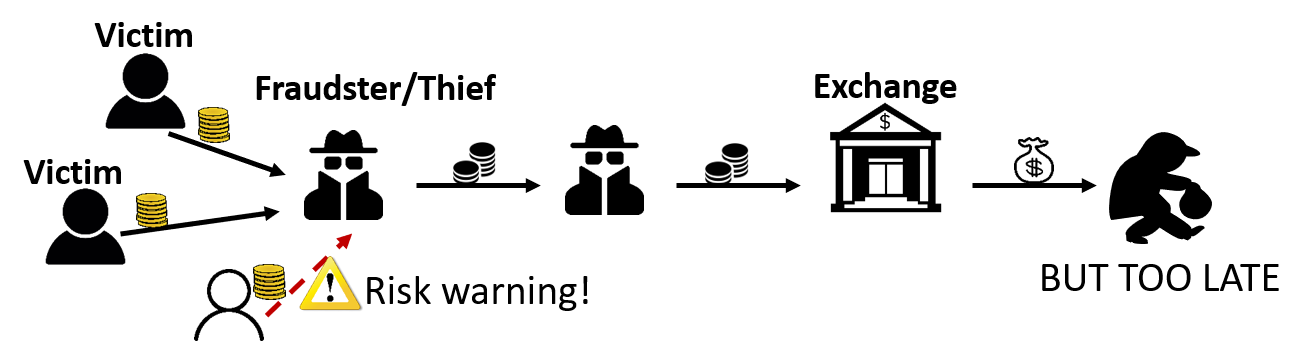
\includegraphics[width=0.8\linewidth]{figures/traditional_fraud_detection.png}
        \label{fig:traditional_fraud_detection}
    }
    
    \subfigure[Remedial money tracking in blockchain]{
        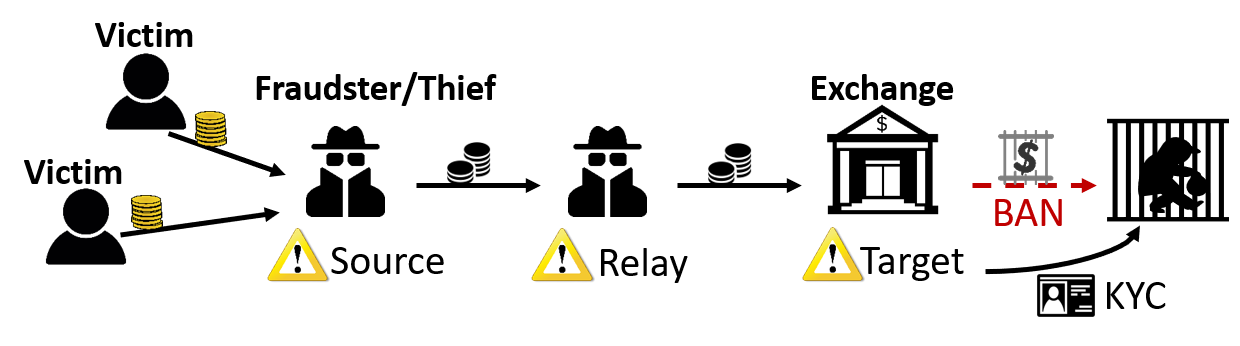
\includegraphics[width=0.8\linewidth]{figures/blockchain_transaction_tracking.png}
        \label{fig:blockchain_transaction_tracking}
    }
    \vspace{-0.1in}
    \caption{(a) Proactive risk warning in blockchain raises warnings for risky transactions. %However, it is always too late to prevent criminals from laundering and cashing out of the ill-gotten gains from exchanges. 
    (b) Remedial money tracking in blockchain traces the money flow among the source and the targets possessing the laundered funds, also providing evidence to catch the criminals off-chain.}
    % 不足以阻止已发生的损失
    \vspace{-0.1in}

\end{figure}

% 区块链交易系统上开展交易追踪的挑战
% Yet transaction tracking on blockchain trading systems is a rather challenging task.
% \textbf{\textit{Firstly}}, because of the pseudonymous nature of blockchain, it is unlikely to enforce the KYC process to verify the identities and ascertain the potential risks of users during cryptocurrency transactions \cite{wu2021analysis}, which makes it extremely difficult to determine the flow direction of a certain amount of money.
% \textbf{\textit{Secondly}}, without identity information, conducting money tracking in a large amount of blockchain transaction records is like finding a needle in the haystack, which requires a low computational cost of the transaction tracking.

% 当前工作的问题
% Current approaches for blockchain transaction tracking \cite{zhao2015graph,phetsouvanh2018egret,oggier2020ego} are mainly based on the Bitcoin system and inspired by graph searching \cite{xu2004fighting,abiteboul2003adaptive} and taint analysis \cite{moser2014towards,tironsakkul2019probing} technologies.
% The main idea of existing studies is to start from the source node and search the possible paths of funds between the source and target nodes via certain rules.
Current approaches for blockchain transaction tracing \cite{zhao2015graph,phetsouvanh2018egret,oggier2020ego,tironsakkul2019probing} are mainly based on rule-based heuristics and taint analysis~\cite{moser2014towards}. 
However, as an emerging research topic, existing transaction tracing methods have limitations in terms of universality, effectiveness and efficiency. Particularly, most existing heuristic methods are designed for specific scenarios based on experts experience, and cannot be automatically and intelligently applied to various blockchain transaction scenarios. In addition, the time cost and end conditions of existing methods, especially those requiring manual verification and intervention, is not definite or well defined, making their time efficiency and effectiveness difficult to guarantee.
% 然而,大多数现有方法通常依赖于专家经验来针对具体案例进行设计,因此很难自动且智能地适用于各类区块链交易场景(普适性)。此外,现有方法的时间复杂性较高,且没有确定的和well designed end condition,使用它们在巨大的交易网络中时犹如大海捞针一样时间效率和有效性都难以保障。
% However, as a newly emerging area, there still exist some limitations in much of the existing work:
% \textbf{(1)} Without theoretical proofs, the end condition of most of the existing methods relies on experts, which makes it difficult to estimate the computational cost of these methods.
% Therefore, the time cost of running existing transaction tracking methods on a large-scale transaction network may be extremely high when the end condition is not well designed.
% \textbf{(2)} Most of the existing studies are heuristic methods designed for some specific cases, which rely heavily on expert experience. Currently, there is no common framework and evaluation criteria for transaction tracking on blockchain. Therefore, it is difficult to evaluate the universality and superiority of the existing methods.
%However, most of the existing methods are designed for Bitcoin and some specific scenarios like cross-chain transactions \cite{yousaf2019tracing} and mixing transactions \cite{beres2020blockchain,wulei2021www}. 
%And they are inapplicable to deal with the transaction tracing task in account-based blockchain trading systems due to the different transaction models and the dependence on expert experience. 
%Moreover, due to the massive transaction data in account-based blockchains, tracing with the manual analysis method like finding a needle in the haystack. And it is difficult to quickly respond to security incidents. 
Besides, the popularity of DeFi in account-based blockchains like Ethereum and BSC brings many new kinds of semantics to blockchain transaction actions, leading to high barriers to the transaction tracing task.
% Yet transaction tracing in blockchain trading systems is a rather challenging task like finding a needle in the haystack due to the large amount of transaction data.

\begin{figure*}[t]
    \centering
    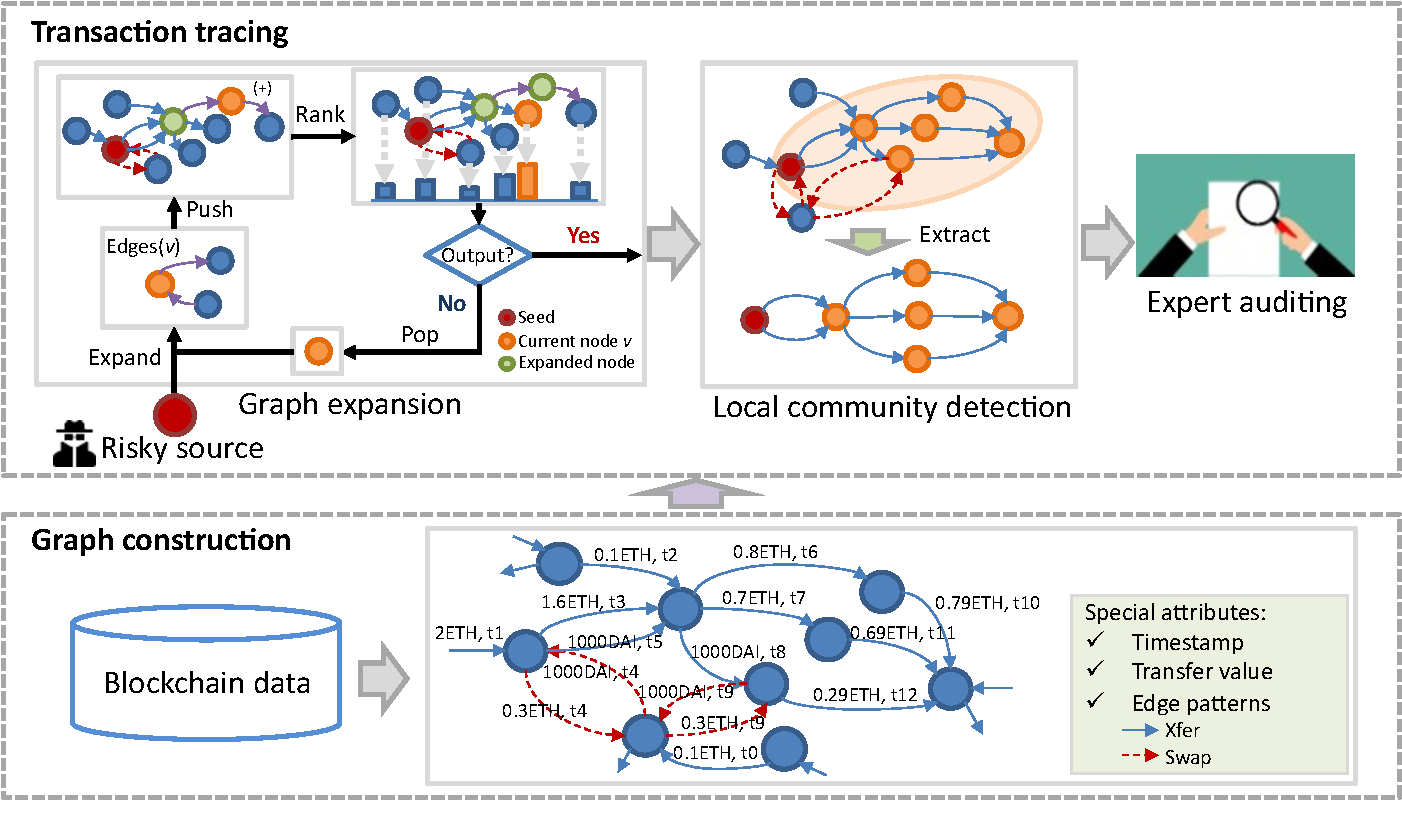
\includegraphics[width=0.65\linewidth]{figures/framework.pdf}
    \caption{The framework of TRacer.}
    \label{fig:TRacer}
\end{figure*}

% 介绍本文的思路
In this paper, we propose the first general tool called \textbf{\underline{T}\underline{R}acer}, which is a transaction \underline{T}racing in account-based blockchain trading systems incorporating Personalized Page\underline{R}ank-based technologies. Referring to the framework displayed in Figure \ref{fig:TRacer}, TRacer first models the blockchain transaction data including the complex DeFi operation actions into a directed, weighted, temporal, and multi-relationship graph, and then conducts local community detection on a subgraph around the risky seed obtained by graph expansion. The output small-scale community is the traced money flow graph and can be further audited by experts.
% Given a source, TRacer can automatically trace the money flow of the source.
% In order to solve the problems above, we propose a general transaction tracking framework on Blockchain trading systems named Push-Pop model, which tracks the fund flow about the source node.
% Then, we design the \textbf{Transaction Tracking Rank} (TTR) algorithm for the Push-Pop model based on personalized PageRank methods, where personalized PageRank is usually used to calculate node importance in a network from a point of view of a given node \cite{page1999pagerank}, ensuring the fund flow paths of the source node and the important nodes in the paths can be found.
% For the challenge brought by the pseudonymous nature, we utilize heuristic knowledge to design the TTR algorithm, so that the target nodes can obtain greater importance for identifying easier.
% we give the definition of transaction tracking on Blockchain trading systems as finding a local tracking network from the source node in which the paths among the source node and the nodes related to the source node can be found, and propose a general transaction tracking framework on Blockchain trading systems named Push-Pop model, which finds a local tracking network from the source node by a specific transaction tracking strategy.
% The transaction tracking strategy decides which nodes can be included in the local tracking network and we design the Transaction Tracking Rank (TTR) algorithm as the transaction tracking strategy of Push-Pop model, which chooses the important nodes of the source node constructing the local tracking network to ensure that the target nodes are more likely to be found in the local tracking network.
% 介绍本文对具体挑战和问题的解决方案
% For the challenge of the pseudonymous nature of Blockchain trading systems, we define the auditability of the local tracking network, which shows that the target nodes can be tracked if they are located in the local tracking network with labels or given in advance.
% 
Moreover, we propose a novel ranking algorithm based on personalized PageRank \cite{page1999pagerank} to reveal the relevance between the source and other accounts in blockchain systems. We introduce approximate personalized PageRank (APPR) \cite{andersen2006local,andersen2007local,yin2017local} to obtain the approximate solution of personalized PageRank, which can improve the scalability of the algorithm. Both graph expansion and local community detection in TRacer are based on the proposed ranking algorithm. 
%For the problems of effectiveness quantification, we design some metrics for understanding what kind of transaction tracking methods are effective. 
% It is worth mentioning that our proposed method has been applied and evaluated in transaction tracking tasks on several blockchain trading systems including Bitcoin, Ethereum, and Binance Smart Chain \cite{binancesmartchain} and so on, but may not be suitable for some privacy-enhancing blockchain trading systems like the Monero \cite{noether2014monero}. % 这些匿名系统都是UTXO上的
% Finally, we evaluate our method with metrics and network visualization analysis on five Ethereum transaction tracing cases.
Experimental results demonstrate the performance of TRacer on transaction tracing in account-based blockchains. The main contributions of this work can be summarized as follows:
\begin{itemize}
    % \item \textbf{Problem}: We give a problem definition of transaction tracking on Blockchain trading systems as finding the paths among the source node and the target nodes, and propose a general transaction tracking model named Push-Pop model.
    \item To the best of our knowledge, we are the first to study intelligent transaction tracing in account-based blockchain trading systems like Ethereum, which is an urgent problem with the booming security incidents in these systems.
    % \item \textbf{Approach}: We propose the TTR algorithm running on a transaction network, whose cost for convergence is $O(\frac{1}{\epsilon \alpha})$ controlled by two constant parameters of $\epsilon$ and $\alpha$. Additionally, we give the theoretical proof on how to set the parameters for ensuring our method is able to track the paths among the source node and the target nodes, even in the face of the worst conditions.
    \item We design and implement a general blockchain transaction tracing tool named TRacer, which is able to incorporate the complex semantics of transaction actions in DeFi. Particularly, a novel personalized PageRank method is employed to estimate the relevance score of accounts in TRacer.
    % \item \textbf{Evaluation}: We introduce metrics to quantify the effectiveness of transaction tracking methods on Blockchain trading systems, and experimental results demonstrate the priority of the proposed method. Moreover, we collect five standard datasets in Ethereum from real cases for blockchain transaction tracking and anti-money laundering research, and these codes for experiments were published on our Github\footnote{https://github.com/wuzhy1ng/BlockchainSpider}.
    % We thoroughly evaluate the proposed approach by comparing with the existing benchmarks on the historical loan data and achieved state-of-the-art performance. In addition, we conduct empirical studies in real-world risk control applications, and the result proves our method could prevent major financial losses for the financial institution
    \item We thoroughly evaluate the performance of TRacer via both theoretical analysis and experimental evaluation, and the results demonstrate the effectiveness and the scalability of TRacer. We also contribute a benchmark dataset verified by several security companies for evaluating the transaction tracing methods.
\end{itemize}

% 文章安排
% The rest of this paper is organized as follows. 
% Section \ref{sec:preliminaries} provides the preliminaries about this paper.
% A general transaction tracking framework Push-Pop model and the Transaction Tracking Rank algorithm are introduced in Section \ref{sec:proposed_approach}. 
% Evaluation and results are presented and discussed in Section \ref{sec:experiments}. 
% In Section \ref{sec:conclusion}, we conclude the paper and suggest directions for future work.
% Citations and appendices are at the end of this paper.
% \begin{figure}[htb]
%     \centering
%     \subfigure[A non-auditable transaction network]{
%         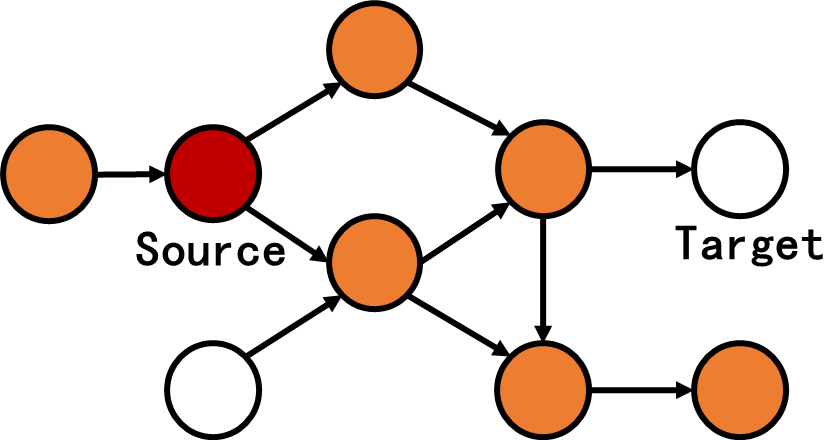
\includegraphics[width=0.46\linewidth,height=2cm]{figures/useless_tracking.png}
%         \label{fig:useless_tracking}
%     }
%     \subfigure[An auditable transaction network]{
%         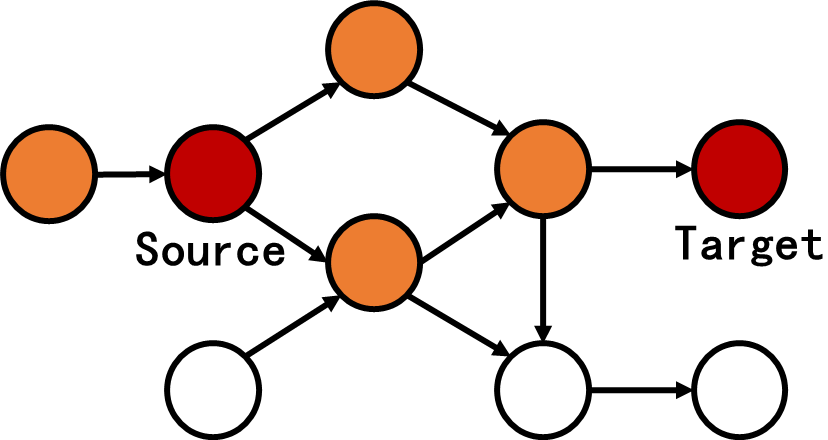
\includegraphics[width=0.46\linewidth,height=2cm]{figures/useful_tracking.png}
%         \label{fig:useful_tracking}
%     }
%     \caption{\color{red} Transaction networks with a source node as the center, where the local tracking network is colored.}
% \end{figure}

% In order to solve the cost problems, we propose heuristic knowledge to improve the local push procedure of the personalized PageRank (PPR) algorithms \cite{haveliwala2003topic,andersen2006local,andersen2007local,yin2017local,zhang2016approximate} for transaction tracking to achieve low-cost transaction tracking with theoretical proof, where PPR methods make a great difference in fraud detection \cite{van2017gotcha, ma2018graphrad} and graph neural networks \cite{klicpera2018predict,bojchevski2020scaling}.
% For the problems of how to quantify the effectiveness, we design some metrics for understanding what kind of transaction tracking methods is effective.

% 本文贡献
% Integrating the ideas above, we propose a general transaction tracking model named Push-Pop model, design the Transaction Tracking Rank (TTR) algorithm for calculating the personalized PageRank with heuristic knowledge proposed, and construct a TTR-based Push-Pop model for effective transaction tracking.


% ------------------我是一条分割线------------------------
% v1.0
% 介绍区块链
% For the past few years, Blockchain systems such as Bitcoin \cite{nakamoto2008bitcoin} have been gaining increasing popularity and attention, which provides a decentralized environment for transactions of cryptocurrencies.
% As the fundamental technology of cryptocurrency, Blockchain combines peer-to-peer (P2P) technology, cryptography, and consensus protocol, and allows the users to participate in transactions with pseudonymous accounts.
% With decentralized, traceable, immutable, and transparent nature, Blockchain is expected to be critical in the ``trust economy" of the future \cite{zhao2021temporal}.

% 介绍区块链上的犯罪现象
% However, the pseudonymous nature of Blockchain also attracts many illicit transaction activities like scams, extortion, money laundering, and so on.
% According to the statistics of Peckshield \cite{peckshield2021aml}, in the first half of 2021 alone, the losses caused by illegal transaction activities in cryptocurrency industry have exceeded \$14.24 billion. 
% % At the same time, cryptocurrency has gradually become a financing channel for terrorist organizations.
% Different from the traditional financial system, it is unlikely to enforce Know-Your-Customer (KYC) processes to verify the identities and ascertain the potential risks of users before conducting a cryptocurrency transaction \cite{wu2021analysis}, which makes it extremely difficult to audit the transactions on Blockchain.

% 监管者的解困之法-交易追踪
% On the other hand, the openness of transaction records on Blockchain also made a great difference in countering the illegal transaction activities on the Blockchain.
% Recent years have witnessed that researchers build transaction records on Blockchain as a transaction network and track the fund involved in illegal activities through transaction tracking technology to help victims recover their fund.

% 现有技术的总结和问题
% Current approaches \cite{zhao2015graph,phetsouvanh2018egret,xu2004fighting,oggier2020ego} for transaction tracking on Blockchain are mainly inspired by the graph searching \cite{xu2004fighting,abiteboul2003adaptive} and taint analysis \cite{moser2014towards,tironsakkul2019probing} technologies.
% And the main idea is to start from the source node and search the possible paths of fund among the source node and the target nodes through certain rules.
% Although the existing approaches are able to track the fund flow of some cases, there are still some key problems to be solved.
% \textit{Firstly}, without theoretical proofs, the end condition of most of the existing methods relies on experts, which makes it difficult to estimate the cost of methods.
% Therefore, existing transaction tracking methods search the transaction network on a large-scale with an extremely high cost if the end condition without well designed.
% \textit{Secondly}, the current researches have not given a standard about what kind of transaction tracking methods is powerful.
% In fact, the majority of methods verify their effectiveness in specific cases without considering the definition of metrics for quantifying the effectiveness of transaction tracking methods.

% \begin{figure*}[htb]
%     \centering
%     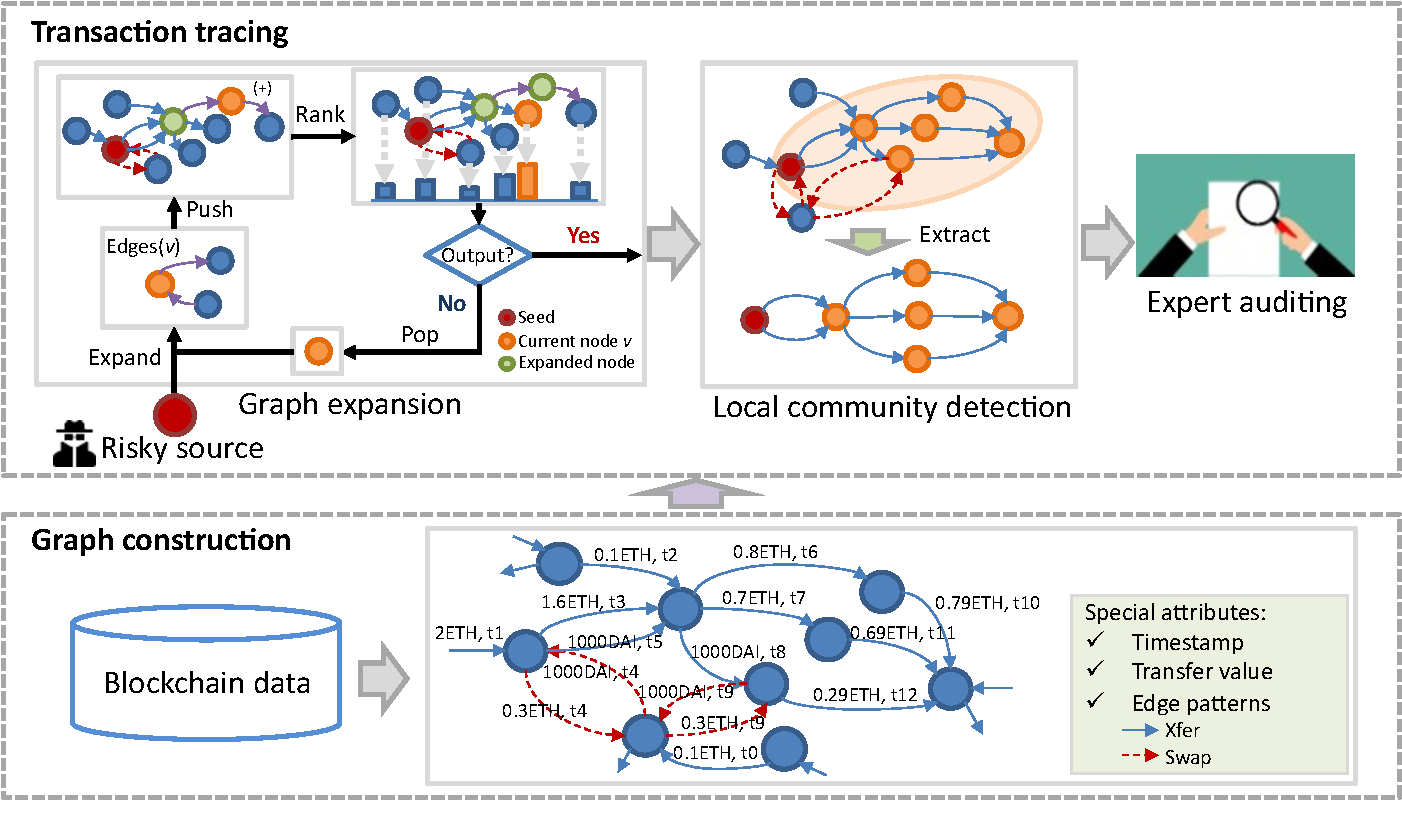
\includegraphics[width=\linewidth]{figures/framework.pdf}
%     \caption{Push-Pop Model, the general transaction tracking framework}
%     \label{fig:framework}
% \end{figure*}

% 顺带介绍一下APPR
% In order to solve the above problems, we have to introduce the personalized PageRank (PPR) \cite{haveliwala2003topic} that estimates the importance of other nodes to the source node in a given network.
% Vlasselaer et al. \cite{van2017gotcha} used PPR in social security fraud detection.
% Approximate Personalized PageRank (APPR) algorithms \cite{andersen2006local,andersen2007local,yin2017local,zhang2016approximate} can calculate the importance of the nodes in the local network to the source node with extremely low cost.
% Ma et al. \cite{ma2018graphrad} used APPR to find local fraud communities on large-scale networks.
% APPR also makes a difference in graph neural network.
% Compared with the original GCN, the performance of the APPR-based graph neural network gets an improvement significantly \cite{klicpera2018predict,bojchevski2020scaling}.

% 提出本文的方法
% Integrating the heuristic knowledge and the Approximate Personalized PageRank algorithm, we proposed our method named Transaction Tracking Rank (TTR), which evaluates the importance of each node for the source node in the transaction network of Blockchain.
% In addition, we give a general transaction tracking framework as the showing of Figure \ref{fig:framework} named as Push-Pop model.
% Our contribution could be listed as follow:
% \begin{itemize}
%     \item Based on the heuristic knowledge, we propose the TTR algorithm running on transaction network, whose cost for convergence within $O(\frac{1}{\epsilon \alpha})$ controlled by two constant parameters of $\epsilon$ and $\alpha$.
%     \item We design a general transaction tracking framework named as Push-Pop model for tracking the paths among the source node and the target nodes.
%     \item Using TTR as the strategy of the Push-Pop model, we give the upper bound of tracking depth starting from the source node and the condition of tracing from the source node to the target node in the worst case with theoretical proofs.
%     \item We give the metrics for understanding what kind of transaction tracking models is effective and the experiments with cases on Ethereum for verifying the effectiveness of our methods.
% \end{itemize}

% 行文思路
% The rest of this paper is organized as follows. 
% Section \ref{sec:preliminaries} gives the preliminaries about this paper.
% A general transaction tracking framework Push-Pop model and the Transaction Tracking Rank  are introduced in Section \ref{sec:proposed_approach}. 
% Evaluation and results are presented and discussed in Section \ref{sec:experiments}. 
% In Section \ref{sec:conclusion}, we conclude the paper and suggest directions for future work.
% Citations at the end of this paper.
%摘要包括:区块链交易网络上交易追踪的重要性,挖掘局部交易网络对下游任务有益,现有研究不足以支撑区块链交易网络上的资产追踪需求,基于什么思路我们提出了怎样的算法,算法在实验中达到了怎样的效果
% Old
% Due to the pseudonymous nature of blockchain, various cryptocurrency systems like Bitcoin and Ethereum have become a hotbed for illegal transaction activities. The ill-gotten profits on many blockchain trading systems are usually laundered into concealed and ``clean'' fund  before being cashed out. Recently, in order to recover the stolen fund of users and reveal the real-world entities behind the transactions, much effort has been devoted to tracking the flow of funds involved in illegal transactions. However, current approaches are facing difficulty in estimating the cost and quantifying the effectiveness of transaction tracking.
% This paper models the transaction records on blockchain as a transaction network, tackle the transaction tracking task as graph searching the transaction network and proposes a general transaction tracking model named as Push-Pop model. 
% Using the three kinds of heuristic designs, namely, tracking tendency, weight pollution, and temporal reasoning, we rewrite the local push procedure of personalized PageRank for the proposed method and name this new ranking method as Transaction Tracking Rank (TTR) which is proved to have a constant computational cost.
% The proposed TTR algorithm is employed in the Push-Pop model for efficient transaction tracking.
% Finally, we define a series of metrics to evaluate the effectiveness of the transaction tracking model. 
% Theoretical and experimental results on realist Ethereum cases show that our method can track the fund flow from the source node more effectively than baseline methods.

Security incidents such as scams and hacks, have become a major threat to the health of the blockchain ecosystem, causing billions of dollars in losses each year for blockchain users.
% Due to the pseudonymous nature of blockchain, it is difficult to reveal the real-world entities behind the blockchain transactions and recover the stolen funds from the massive transaction data. Recently, much effort has been devoted to tracing the flow of funds involved in illegal transactions.
To reveal the real-world entities behind the pseudonymous blockchain account and recover the stolen funds from the massive transaction data, much effort has been devoted to tracing the flow of illicit funds in blockchains recently.
However, most current tracing approaches based on heuristics and taint analysis have limitations in terms of universality, effectiveness, and efficiency. This paper models the blockchain transaction records as a blockchain transaction graph and tackles blockchain transaction tracing as a graph searching task. 
We propose \textbf{TRacer}, a scalable transaction tracing tool for account-based blockchains. 
To infer the relevance between accounts during graph searching, we develop a novel personalized PageRank method in TRacer based on the directed, weighted, temporal, and multi-relationship blockchain transaction graphs. 
To the best of our knowledge, TRacer is the first intelligent transaction tracing tool in account-based blockchains that can handle complex transaction actions in decentralized finance (DeFi).
Experimental results and theoretical analysis prove that TRacer can complete the transaction tracing task effectively at a low cost. 
All codes of TRacer are available at GitHub \footnote{https://github.com/wuzhy1ng/BlockchainSpider}.
% , whose data come from the open APIs \footnote{https://blockscan.com/} ensuring everyone to trace the illicit funds in the account-based blockchains without deployment.
\section{Preliminaries} 
\label{sec:preliminaries}
% Before introducing our method, this section discusses the problem definition and provides preliminaries for this paper.

\subsection{Account-based blockchains}
% 不同于比特币系统采用基于UTXO的交易模型,以以太坊为首的基于账户的区块链系统xxxx
% 智能合约  DApp
% 由DApp引出Token  Token标准
% 去中心化交易所
Traditional Bitcoin-like blockchains are based on the transaction-centered model \cite{wu2021analysis} whose building block is unspent transaction output (UTXO), which is an indivisible cryptocurrency chunk locked to a specific owner. Each transaction has multiple inputs made up of UTXOs and multiple outputs, and there is a change address in the outputs used to receive the change.

Different from UTXO-based blockchains, account-based blockchain systems like Ethereum and BSC have the concept of account similar to that of traditional banking accounts. 
There are two kinds of accounts in account-based blockchains, namely external owned account (EOA) and smart contract account. 
Accounts are the initiators of blockchain transactions and record some dynamic state information including account balance. 
Especially, each smart contract account is associated with a piece of executable bytecode. There are also two types of transactions in the systems. 
A transaction triggered by an EOA is called external transaction, while a transaction triggered by an invocation of the function in a smart contract account is called internal transaction. 
In addition, an EOA can invoke functions of a smart contract in an external transaction and further result in many internal transactions. Transaction hash consisting of a set of numbers and letters is used to uniquely identify a particular transaction from or to an EOA.
Due to the support of smart contract, everyone can take the advantage of blockchain technology and build DApp projects in account-based blockchains.
Besides the native currency in blockchain systems, there are many third-party tokens representing assets, currency, or access rights of projects in the account-based blockchain ecosystem. 
To facilitate token development and exchange, some token standards are launched in blockchain trading systems, e.g., the ERC20 token standard in Ethereum. 
There are also many DeFi DApps that offer financial services such as token lending and exchange.
% 原来:
% 介绍加密数字货币包括原生币和Token
% There are two types of cryptocurrencies in account-based blockchains: native token and third-party token complimenting some standards.
% For Ethereum, the native token Ether and 
% 介绍什么是DeFi,DeFi世界中的交易语义有哪些

\subsection{Problem Definition}
\label{sec:problem_define}
The transaction tracing task in account-based blockchain trading systems aims to trace the money flows from a given source to the targets that gather the money awaiting cashing out and point the priority money flows for auditors to further verify manually. By modeling the blockchain transaction relationships as graph where nodes indicate the accounts and edges indicate the money flow relationships, we can formulate the transaction tracing problem as follows. 

% \begin{prbdef}
\textbf{Problem formulation.} \textit{Given a source node $s$ in a transaction graph $G$, the goal is to search a connected money transfer subgraph $G_{s}$ from $s$ to its money flow targets around the neighborhood of $s$. $G_{s}$ should contain as many target nodes as possible in the smallest possible size of graph for manual verification.}
% \end{prbdef}
% \textbf{Transaction network}.
% Transaction records on Blockchain trading systems like Bitcoin and Ethereum represent the relationship of cryptocurrency transfer among accounts.
% In this paper, transaction records from blockchain trading systems are represented as a transaction network $G = (V, E)$, where $V$ denotes the node set representing addresses, and $E$ denotes the edge set representing transaction relationships between addresses. 
% \textcolor{red}{Considering the amount, timestamp and token symbol of the transactions, each edge $e \in E$ can be defined as a five-tuple like $(u,v,w,t,b)$, where $u, v \in V$ denote the source and target nodes of $e$, respectively, $w$ denotes the transaction amount, $t$ denotes the transaction timestamp, and $b$ denotes the token symbol.}

% \textbf{Transaction Tracking on Blockchain}.

% The task of transaction tracking on blockchain can be modeled as graph searching on a transaction network, aiming at finding a subgraph of $s$ named \textbf{local tracking network}, denoted by $G_s$, which contains as many target nodes as possible.  
% As mentioned in the introduction, source nodes are usually deployers of various financial scams such as phishing, Ponzi scheme, blackmail, and extortion scams  \cite{wu2021analysis,oggier2020ego}, while the target nodes refer to the addresses which possess the laundered funds awaiting cashing out. 
% Due to the pseudonymous nature of blockchain, it is extremely difficult to trace the money flows between the source and target nodes and understand real-world entities behind the involved addresses and transactions.
% In some cases, some addresses are confirmed to be involved in illegal transaction activities by experts, and then the local tracking network should contain as many of these target nodes as possible.
% While sometimes, no prior information about target nodes is given, and then the local tracking network aims to contain the addresses with some particular labels (such as exchange deposit addresses) that are related to the source, providing us an opportunity to further infer the target nodes from these labeled nodes.


%identify all target nodes from the nodes related to the source node if the target nodes without given before.
% For example, the hackers steal the coin of the exchange, and we need to find the target nodes of hackers through transaction tracking methods.
% In addition, due to the pseudonymous nature of Blockchain trading systems, fetching the identity information for the transaction tracking model to know whether the target nodes have been found without given target nodes before is difficult.
%The goal of the transaction tracking problem can be given as follows:
%\begin{prbdef}

%The goal of this work is to find a network that contains as many nodes and transactions involved in the case as possible.

%Given a source node $s$ and a set of target nodes in a transaction network $G$, the goal of a transaction tracking model is to find a subgraph of $s$ named \textbf{local tracking network}, denoted by $G_s$, that contains as many target nodes as possible.
%\label{def:goal_tt_model}
%\end{prbdef}

% Transaction tracking tasks can be regarded as graph searching tasks on a transaction network, aiming at finding paths among the source node and the target nodes.
% In fact that it is difficult to know the target nodes before the transaction tracking task usually, for example, the hackers steal the coin of the exchange, and we need to find the target nodes of hackers through transaction tracking technology.
% In addition, due to the pseudonymity of transaction records on Blockchain, fetching the identity information of each node in the transaction network is impossible, which makes it difficult for the transaction tracking model to know whether the target node has been found without given target nodes before.

% \begin{prbdef}
% Base on this consideration, our goal is to construct a well-designed transaction tracking model able to find a subgraph named local tracking network from the source node, which satisfies:
% \begin{itemize}
%     \item The paths among the source node and the target nodes can be found, if the targets are given before.
%     \item The paths among the source node and the labeled nodes can be found, if the targets are unknown. 
%     And ensured that the target nodes can be found in the labeled node as much as possible.
% \end{itemize}
% \end{prbdef}

% Base on this consideration, the well-designed transaction tracking model will be able to find a subgraph that is most likely to contain the paths among the source node and the target nodes, even though the target node is not given in advance.
% Such a subgraph can be named a local tracking network.
% In this way, the effectiveness of the transaction tracking model can be evaluated by detecting whether there are enough label nodes in the local tracking network because experts can judge the action of the source node through the label nodes in the local tracking network, and then determine whether the label node is the target node through this action.

% Base on the Definition \ref{def:goal_tt_model}, we define the auditability of the local tracking network.
%According to whether the target nodes in the local tracking network can be identified, the auditability of a transaction network with a center of the source node is given as follow:
%\begin{prbdef}
%A transaction network with a center of the source node can be audited by a local tracking network, which satisfies: \textbf{1)} The paths among the source node and the target nodes can be found if the target nodes are given before. \textbf{2)} The paths among the source node and the labeled nodes can be found if the target nodes without given before, where the target nodes can be inferred from the labeled nodes.
% \end{itemize}
%\end{prbdef}
%For example, when it comes to a source node obtaining an amount of illegal money, laundering the money in a blockchain system and cashing them out via an exchange, the target node is the corresponding exchange deposit address without being given before. And we need to find out the paths between them.
%The transaction network can not be audited by the local tracking network in Figure \ref{fig:useless_tracking}, which misses the paths among the source and the target.
%On the contrary, the transaction network can be audited by the local tracking network as the Figure \ref{fig:useful_tracking}, which finds the path from the source to the target.

% It's reasonable that node $t$ is a target node of the source node $s$, because the stolen fund can be laundered on the exchange.
% There is a useless local tracking network as the Figure \ref{fig:useless_tracking} shows, which misses the path among $s$ and the labeled nodes, and we will not get more information from such a local tracking network about the target nodes of $s$.
% On the contrary, the local tracking network in Figure \ref{fig:useful_tracking} finds the path from $s$ to $t$, which is helpful for us to identify the target nodes.

% For example, when it comes to a source node $s$ obtaining the illegal fund and transfers the illegal fund to a node $t$ labeled as exchange.
% It's reasonable that node $t$ is a target node of the source node $s$, because the stolen fund can be laundered on the exchange.
% There is a useless local tracking network as the Figure \ref{fig:useless_tracking} shows, which misses the path among $s$ and the labeled nodes, and we will not get more information from such a local tracking network about the target nodes of $s$.
% On the contrary, the local tracking network in Figure \ref{fig:useful_tracking} finds the path from $s$ to $t$, which is helpful for us to identify the target nodes.

% In a word, the problem in this paper is how to design a transaction tracking model to complete the transaction tracking task in transaction networks on Blockchain.
% Here gives the definition of transaction tracking task as follow:\\
% \textbf{Definition}.
% \textit{Giving a transaction network $G$ and a source node $s$, the transaction tracking task is finding a local tracking network of $s$ that contains the paths among the source node and the target nodes.
% If the target nodes are unknown, ensured that the target nodes can be found in the labeled nodes of local tracking network as much as possible.}
% \begin{itemize}
%     \item If the target nodes are given, the transaction tracking task is finding a local tracking network of $s$ that contains the paths among the source node and the target nodes.
%     \item If the target nodes are unknown, the transaction tracking task is finding a local tracking network of $s$ that contains the paths among the source node and the labeled nodes ensured that the target nodes can be found in the labeled node as much as possible.
% \end{itemize}

\subsection{Approximate Personalized PageRank}
% To ensure the effectiveness of the tracking model, we usually need to define an importance measurement of other nodes in the network to the source node.
% or the probability of random walk to $u$ starting from $s$
\textbf{Personalized PageRank.} The personalized PageRank vector $\bm{p}_s$ of a source node $s$ in a graph $G=(V,E)$ is defined as the unique solution of Equation \ref{equ:ppr}, i.e.,
\begin{equation}
    \bm{p}_s = \alpha \bm{e}_s + (1-\alpha) \bm{p}_s M,
    \label{equ:ppr}
\end{equation}
where $\alpha$ is a teleport constant between 0 and 1, $\bm{e}_s$ is the indicator vector with a single nonzero element of 1 at $s$, $M$ is a transition matrix and $M=D^{-1}A$ where $D$ and $A$ are degree matrix and adjacency matrix. The definition of personalized PageRank is equivalent to simulating a random walk starting from $s$, and $\bm{p}_s$ is a probability vector where $\bm{p}_s(u)$ is the probability that a certain random walk beginning at $s$ terminates at $u$. 
% Let $\bm{p}_s$ denote the personalized PageRank vector of a source node $s$ in a graph $G=(V,E)$, where $\bm{p}_s(u)$ describes the relevance of a node $u$ to the source node $s$.

\textbf{Approximate personalized PageRank (APPR).} The first algorithm proposed to calculate personalized PageRank is power iteration \cite{page1999pagerank}, which requires high time complexity and not effective in large-scale networks.
Therefore, various efficient approximate solutions of personalized PageRank have been proposed, and the most widely used one is called the ``local push'' algorithm \cite{andersen2006local}. This algorithm starts with all probability residual on the source node of the graph, and pushes the residual to the neighbors iteratively. During the iterations, the residual of each node can be transformed into the relevance to the source node. Finally an estimate of $\bm{p}_s$ can be obtained. In the algorithm, a residual vector $\bm{r}_s$ is used to maintain the residual, where $\bm{r}_s(u)$ denotes the residual of node $u$. By setting $\bm{p}_s=\vec{0}$ and $\bm{r}_s=\bm{e}_s$ for initialization, the local push procedure updates the value of $\bm{p}_s(u)$ as follows:
\begin{equation}
    \begin{cases}
    & \bm{p}_s(u)=\bm{p}_s(u)+\alpha \bm{r}_s(u) \\
    & r(v)=r(v)+(1-\alpha)r(u) / d(u), \\
    % & \bm{r}_s(v)=\bm{r}_s(u)+\theta(u,v)\bm{r}_s(u)
    \end{cases},
    \label{equ:local_push_appr}
\end{equation}
where $v \in N(u)$ is the neighbor of $u$, and 
% the push factor $\theta(u,v)$ between $u$ and $v$ is defined as
% \begin{equation}
%     \theta(u,v)=\frac{1-\alpha}{d(u)},
% \end{equation}
% where 
$d(u)$ is the degree of $u$.
The local push procedure stops when the residual of each node in $G$ is within $\epsilon$.

\section{Appendices}

\subsection{Proof of Theorem \ref{thm:run_time}}
\begin{proof}
This follows from Andersen et al. \cite{andersen2006local}, Lemma 2.
\end{proof}

\subsection{Proof of Theorem \ref{thm:push_cost}}
\begin{proof}
The residual of a node $u$ coming from its neighbors ensures that the number of non-zero elements in $R_s(u)$ are less than $|E(u)|$, where $E(u)$ contains edges related to $u$, so the cost of selfPush will not exceed $O(E(u))$.
In addition, forwardPush and backwardPush are both related to the timestamp of edges, so all edges among node $u$ and its neighbors can be sorted according to their timestamp firstly, whose cost is $O(|E(u)|log(|E(u)|))$, and then the summation terms are calculated in a timestamp order, whose cost is $O(|E(u)|)$.
Therefore, the cost of the local push procedure is:
\begin{equation}
    O( |E(u)|log(|E(u)|) + |E(u)| ) = O(|E(u)|log(|E(u)|)).
\end{equation}
\end{proof}

\subsection{Proof of Proposition \ref{pot:ttr_max_height}}
\begin{proof}
In order to maximize the estimate of $\bm{p}_s$ for the nodes having a high order of the source node, $\alpha$ needs to be as small as possible, and $\beta$ needs to be as close as possible to 0 or 1, which ensures that the residual can be pushed to a specific direction.
%  for reducing the dissipation caused by shunting
Considering $\beta=1$ here, the sum of residual pushed from the source node $s$ to the neighbors of order 1 to order $n$ are:
\begin{equation}
    \begin{cases}
        & r^{(1)}=(1-\alpha), \\
        & r^{(2)} \geq (1-\alpha)(r^{(1)}-k_1 \epsilon)=(1-\alpha)^2-(1-\alpha)k_1 \epsilon, \\
        & ...... \\
        & r^{(n)} \geq (1-\alpha)(r^{(n-1)}-k_{n-1} \epsilon) \\
        & \ \ \ \ \ \ \ \ =(1-\alpha)^n-\sum\limits_{i=1}^{n-1}(1-\alpha)^{n-i}k_{n-i} \epsilon, \\
    \end{cases}
\end{equation}
where $k_i$ represents the number of nodes with residual less than $\epsilon$ in the $i$-order neighbors of the source node.
Therefore, $r^{(n)}$ obtains the maximum value when:
\begin{equation}
    \sum\limits_{i=1}^{n-1}(1-\alpha)^{n-i}k_{n-i} \epsilon = 0,
\end{equation}
which means the residual of each $i$-order node greater or equal than $\epsilon$. 
This situation exists when the source node in a path graph, whose adjacency matrix satisfies $A(i,i+1)=1$ and other elements are $0$.
Consider the end condition of the local push procedure, the residual of $n$-order neighbors is:
\begin{equation}
    r^{(n)}=(1-\alpha)^n \leq \epsilon \Rightarrow n \leq \frac{log(\epsilon)}{log(1-\alpha)}.
\end{equation}
\end{proof}

\subsection{Proof of Proposition \ref{pot:ttr_local_comm}}
\begin{proof}
Consider the end condition of TTR-based Local Community Discovery Algorithm:
\begin{equation}
    \Phi(S)=\frac{\bm{p}_s(\partial(S))}{\bm{p}_s(S)} < \varphi,
\end{equation}
and the selfPush procedure at the first iteration of TTR Algorithm ensures:
\begin{equation}
    \bm{p}_s(s) \geq \alpha.
\end{equation}
Since $s \in S$, then $\bm{p}_s(S) \geq \alpha$, so:
\begin{equation}
    \bm{p}_s(\partial(S))<\varphi \alpha,
\end{equation}
which means that the path between $s$ and $v_n$ must be included in the local tracking network when $\bm{p}_s(v_n) \geq \varphi \alpha$. 
In this way, $\bm{p}_s(v_n)$ can obtain a minimum value with only one selfPush operation for $v_n$, and then $\bm{p}_s(v_n) \geq \varphi \alpha$ needs:
\begin{equation}
    % \alpha \sum_t r(v_n)(t) \geq \varphi\alpha \\
% \Rightarrow \sum_t r(v_n)(t) \geq \varphi.
    \alpha ||R_s(v_n)|| \geq \varphi \alpha \Rightarrow ||R_s(v_n)|| \geq \varphi
\label{equ:proof_ttr_local_comm_phi_target}
\end{equation}
Moreover, in order to ensure that at least one selfPush operation on $v_n$, the residual of $v_n$ must be greater than $\epsilon$, that is:
\begin{equation}
    \varphi \geq \epsilon.
\end{equation}
Consider that satisfying Equation \ref{equ:proof_ttr_local_comm_phi_target} in the worst case: 
1) The path between the source node and a target node is weakly connected, which makes the tracking tendency invalid.
2) The edges related to each node on the paths among the source node and the target node have the same weight, which makes the weight pollution invalid. 
3) Each path between the source node and a target node without increasing or decreasing timestamp, which makes time reasoning invalid.
4) There is only one path between the source node and a target node.
In this case, in order to satisfy the Equation \ref{equ:proof_ttr_local_comm_phi_target}, the residual sum of $m$-order neighbors ($m \leq n$) of the target node $v_n$ are:
\begin{equation}
    \begin{cases}
        & r^{(n)} \geq \varphi, \\
        & r^{(n-1)} \geq \frac{\varphi d_{n-1}}{min(\beta,1-\beta)(1-\alpha)}, \\
        & r^{(n-2)} \geq \frac{\varphi d_{n-1}d_{n-2}}{min^2(\beta,1-\beta)(1-\alpha)^2}, \\
        & ......\\
        & r^{(n-m)} \geq \frac{\varphi \prod\limits_{i=1}^{m}d_{n-i}}{min^m(\beta,1-\beta)(1-\alpha)^m},
    \end{cases}
\end{equation}
where $d_{n-i}$ denotes the degree of the $n-i$ order node in this path.
Consider the inequality as follow:
\begin{equation}
    \prod\limits_{i=1}^{m}d_{n-i} \leq (\frac{1}{m}\sum\limits_{i=1}^{m}d_{n-i})^m \rightarrow \bar{d}^m.
\end{equation}
If the $m$-order neighbor of the target node is the source node, then:
\begin{equation}
    1 \geq \frac{\varphi \bar{d}^n}{min^n(\beta,1-\beta)(1-\alpha)^n}
\Rightarrow \bar{d}\varphi^{\frac{1}{n}} \leq (1-\alpha) \cdot min(\beta,1-\beta)
\end{equation}
\end{proof}
\section{Conclusion}
\label{sec:conclusion}
In this paper, we studied the transaction tracing problem on account-based blockchain trading systems and proposed the first intelligent transaction tracing tool named TRacer. Compared with existing methods based on heuristics and taint analysis, which usually requires expert experience and manual intervention, TRacer show obvious superiority in terms of universality, effectiveness and time cost. In TRacer, we first formulated the transaction records in each account-based blockchain as a directed, weighted, temporal, and multi-relationship graph, which is able to represent the rich semantics of complex multi-token transaction relationships in the system. Then we proposed to use personalized PageRank-based graph searching technologies on this complex graph to trace the money flows. Specifically, we introduced novel approximate personalized PageRank strategies to realize effective and low-cost transaction tracing, which can also handle the complex DeFi transaction actions in account-based blockchains. The theoretical analysis and experimental results demonstrated the effectiveness of TRacer. 
% However, TRacer still cannot trace the fund flow using privacy enhancement technology, especially the mixing services such as Tornado Cash.
In the future, we will further delve into blockchain transaction tracing by integrating more transaction features like bytecodes and logs and design effective methods for blockchain systems with privacy-enhancing mechanisms.
% Moreover, our method can capture the subgraph of the source node, which will be used to carry out more effective node classification in future work.
\section{Related Work}
To combat crimes in blockchain, transaction tracing is a critical task for blockchain security companies and the community. Current methods for blockchain transaction tracing are mainly designed for Bitcoin-like blockchain systems and heavily rely on expert experience. The most widely used transaction tracing method is Breath First Search (BFS) \cite{zhao2015graph,phetsouvanh2018egret}, and many related tools like skytrace\footnote{https://www.certik.com/skytrace} and coinholmes\footnote{https://trace.coinholmes.com} are available. Since BFS is insufficient to reveal the audit priority of different money tracking directions, the taint analysis technologies \cite{moser2014towards,tironsakkul2019probing,di2015bitconeview} have been proposed for bitcoin tracing according to the amount value and the order of multiple outputs in each transaction. However, these technologies rely on expert analysis and cannot automatically output the money flows from the source to the targets.

Based on the co-spending clustering heuristic in Bitcoin that the input addresses of the same transaction belong to the same entity \cite{Reid2013}, Huang et al. proposed to track the bitcoin flow of ransomware to when the money is being cashed out \cite{HuangTracking2018}.
% Tracking Ransomware End-to-end
Meiklejohn et al. \cite{meiklejohn2013fistful} utilized the change address heuristic to deanonymize the money flows in Bitcoin.
Moreover, some rule-based transaction tracing methods were proposed for cross-chain scenarios and mixing scenarios. For example, Yousaf et al. traced the cross-chain money flows by identifying the transactions which happen close in time and have similar amount value \cite{yousaf2019tracing}. 
However, these rule-based methods are designed for specific protocols and they are inapplicable to transaction tracing in account-based blockchains.

Personalized PageRank models the relevance of nodes in a network to a specific node, and has been widely used in web search \cite{page1999pagerank}, recommendations \cite{WTFGupta2013}, etc. Recently many variants and efficient approximations of personalized PageRank have been proposed for large-scale applications \cite{bojchevski2020scaling}. In this paper, we model the account-based blockchain data as a directed, weighted, temporal, and multi-relationship graph, and formalize the transaction tracing problem as a graph searching problem. We develop a scalable and intelligent transaction tracing tool for account-based blockchains based on personalized PageRank and its approximate solutions.
